%%%%%%%%%%%%%%%%%%%%%%%%%%%%%%%%%%%%%%%%%%%%%%%%%%%%%%%%%%%%%%%%%%%%%%%%%%%%%%
% A user guide for semtex spectral element code.
%%%%%%%%%%%%%%%%%%%%%%%%%%%%%%%%%%%%%%%%%%%%%%%%%%%%%%%%%%%%%%%%%%%%%%%%%%%%%%
\documentclass[11pt]{report}

\usepackage{%
graphicx,
natbib,
amsmath,
bm,
cancel,
color,
xfrac,
a4wide
}
\usepackage[colorlinks=true,linkcolor=blue,citecolor=blue]{hyperref}

\graphicspath{{./Figs/}}

\setlength{\textheight}              {245mm}
\setlength{\textwidth}               {160mm}
\setlength{\topmargin}               {-20mm}
\setlength{\oddsidemargin}           {0mm}
\setlength{\parindent}               {2.5ex}
\setlength{\leftmargin}              {2.5ex}
\setlength{\bibsep}                  {\parskip}

\renewcommand{\baselinestretch}      {1.0}
\renewcommand{\familydefault}{cmss}
\renewcommand{\bibname}{References}

\def\bs#1{\mbox{\boldmath$#1$}}                     % bold symbol typeface
\def\vec#1{\mbox{\bf#1}}                            % bold vector typeface
\def\Rey{\mbox{\it Re}}                             % Reynolds number
\def\St{\mbox{\it St}}                              % Strouhal number
\def\Pr{\mbox{\it Pr}}                              % Prandtl number
\def\Ra{\mbox{\it Ra}}                              % Rayleigh number
\def\undertext#1{$\underline{\smash{\hbox{#1}}}$}   % underline running text
\def\refitem{\noindent\hangindent=2em}              % hanging indent

\newcommand{\Semtex}{\emph{Semtex}} \newcommand{\Dog}{\emph{Dog}}
\newcommand{\SM}{\emph{SuperMongo}}
\newcommand{\Tecplot}{\emph{Tecplot}}
\newcommand\qp{qua\-si-per\-io\-dic} \newcommand\cc{complex-conjugate}
\newcommand\oned{one-di\-men\-sion\-al}
\newcommand\twod{two-di\-men\-sion\-al}
\newcommand\threed{three-di\-men\-sion\-al}
\newcommand\twoc{two-com\-po\-nent}
\newcommand\threec{three-com\-po\-nent}
\newcommand{\thalf}{{\textstyle\frac{1}{2}}}
\newcommand\gll{Gauss--Lobatto--Legendre}
\newcommand\real{{\mbox{Re}}} \newcommand\imag{{\mbox{Im}}}
\newcommand\etal{{\it et al}.}  \newcommand{\ie}{i.e.\ }
\newcommand{\eg}{e.g.\ } \newcommand{\CC}{\mathrm{c.c.}}
\newcommand\cd{\mathrm{d}} \newcommand\cD{\mathrm{D}}
\newcommand\ce{\mathrm{e}} \newcommand\ci{\mathrm{i}}
\newcommand\cg{\mathrm{g}}
\newcommand\KH{Kelvin--Helmholtz} \newcommand\Pois{Poiseuille}
\newcommand\HP{Hagen--Poiseuille} \newcommand\Orrsom{Orr--Sommerfeld}
\newcommand\GLL{Gauss--Lobatto--Legendre}
\newcommand\NavSto{Navier--Stokes}
\newcommand\TOKEN{\verb|TOKEN|}
\newcommand\cpp{C\nolinebreak\hspace{-.05em}\raisebox{.3ex}{\footnotesize\bf
+}\nolinebreak\hspace{-.10em}\raisebox{.3ex}{\footnotesize\bf+}}

%%%%%%%%%%%%%%%%%%%%%%%%%%%%%%%%%%%%%%%%%%%%%%%%%%%%%%%%%%%%%%%%%%%%%%%%%%%%%%
\begin{document}

\begin{titlepage}
\centering

\vspace*{\fill}

{\huge Using \Semtex}

\vspace{\fill}

\begin{figure}[h]
\begin{center}
\fbox{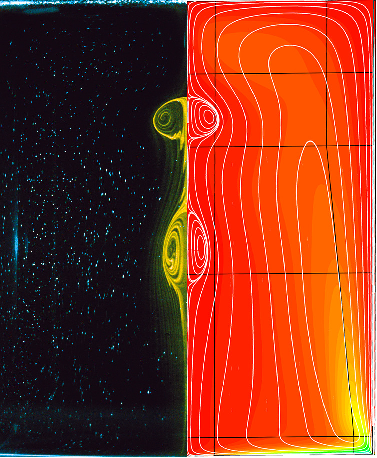
\includegraphics[width=0.5\textwidth]{vbmed_bitmap}}
\end{center}
\end{figure}

\vspace{\fill}

{\large H.\,M. Blackburn}\\
Monash University

\vspace{\fill}

\today

\Semtex\ version 10

\vspace*{\fill}

\end{titlepage}

%%%%%%%%%%%%%%%%%%%%%%%%%%%%%%%%%%%%%%%%%%%%%%%%%%%%%%%%%%%%%%%%%%%%%%%%%%%%%%

\tableofcontents

\clearpage

%%%%%%%%%%%%%%%%%%%%%%%%%%%%%%%%%%%%%%%%%%%%%%%%%%%%%%%%%%%%%%%%%%%%%%%%%%%%%
\chapter{Introduction}
\label{ch.intro}

\Semtex\ is a family of spectral element simulation codes, most
prominently a code for direct numerical simulation of incompressible
flow.  The spectral element method is a high-order finite element
technique that combines the geometric flexibility of finite elements
with the high accuracy of spectral methods.  The method was pioneered
in the mid 1980's by Anthony Patera at MIT
\citep{pat84,kp86}. \Semtex\ uses isoparametrically mapped
\twod\ quadrilateral elements, the classic \GLL\ `nodal' shape
function basis, and continuous Galerkin projection. Extension to
\threed\ capability is achieved using Fourier expansions in an
orthogonal direction.  Algorithmically the code is similar to Ron
Henderson's \emph{Prism} \citep{hk95,kh98,hen99b}, but with some
differences in design, and lacks mortar element capability. A notable
extension is that \Semtex\ can solve problems in cylindrical as well
as Cartesian coordinate systems \citep{blsh04,blas19}.

%-----------------------------------------------------------------------------
\section{Numerical method}

Some central features of the spectral element method are
\begin{description}
\item[Orthogonal polynomial-based shape functions] Spectral accuracy
  is achieved by using tensor-product Lagrange interpolants within
  each element, where the nodes of these shape functions are placed at
  the zeros of Legendre polynomials mapped from the canonical domain
  $[-1,+1]\times[-1,+1]$ to each element.  In one spatial dimension,
  the resulting \GLL\ interpolant which is unity at one of the $N + 1$
  Gauss--Lobatto points $x_j$ in $[-1,+1]$ and zero at the others
  is
\begin{equation}
\psi_j(x) = \frac{1}{N(N+1)L_N(x_j)}\frac{(1-x^2)L_N^\prime(x)}{x_j - x}.
\end{equation}
For example, the family of sixth-order GLL Lagrange interpolants is
shown in figure~\ref{fig:shapes}.
\begin{figure}
\begin{center}
  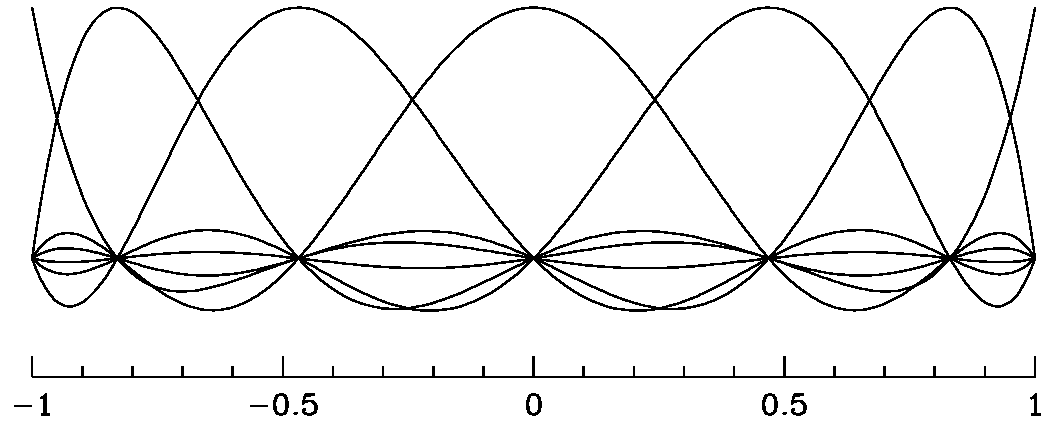
\includegraphics[width=0.5\textwidth]{shape7x7}
\end{center}
\caption{The family of sixth-order \oned\ GLL Lagrange shape functions
  on the master domain $[-1,+1]$.}
\label{fig:shapes}
\end{figure}
In smooth function spaces it can be shown that the resulting
interpolants converge exponentially fast (faster than any negative
integer power of $N$) as the order of the interpolant is increased.
See \citet{chqz88}, \S\S\,2.3.2 and~9.4.3 or \citet{chqz06} \S\,5.4.
\item[Standard finite element isoparametric mapping] Two-dimensional
  element shape functions are constructed as tensor products of
  \oned\ shape functions.  Non-rectangular element shapes, if
  required, are developed using isoparametric mappings between
  physical $(x,y)$ space and master element $(r,s)$ space on the domain
  $[-1,+1]\times[-1,+1]$, as illustrated in figure~\ref{fig.xyrs}.
\begin{figure}
\begin{center}
  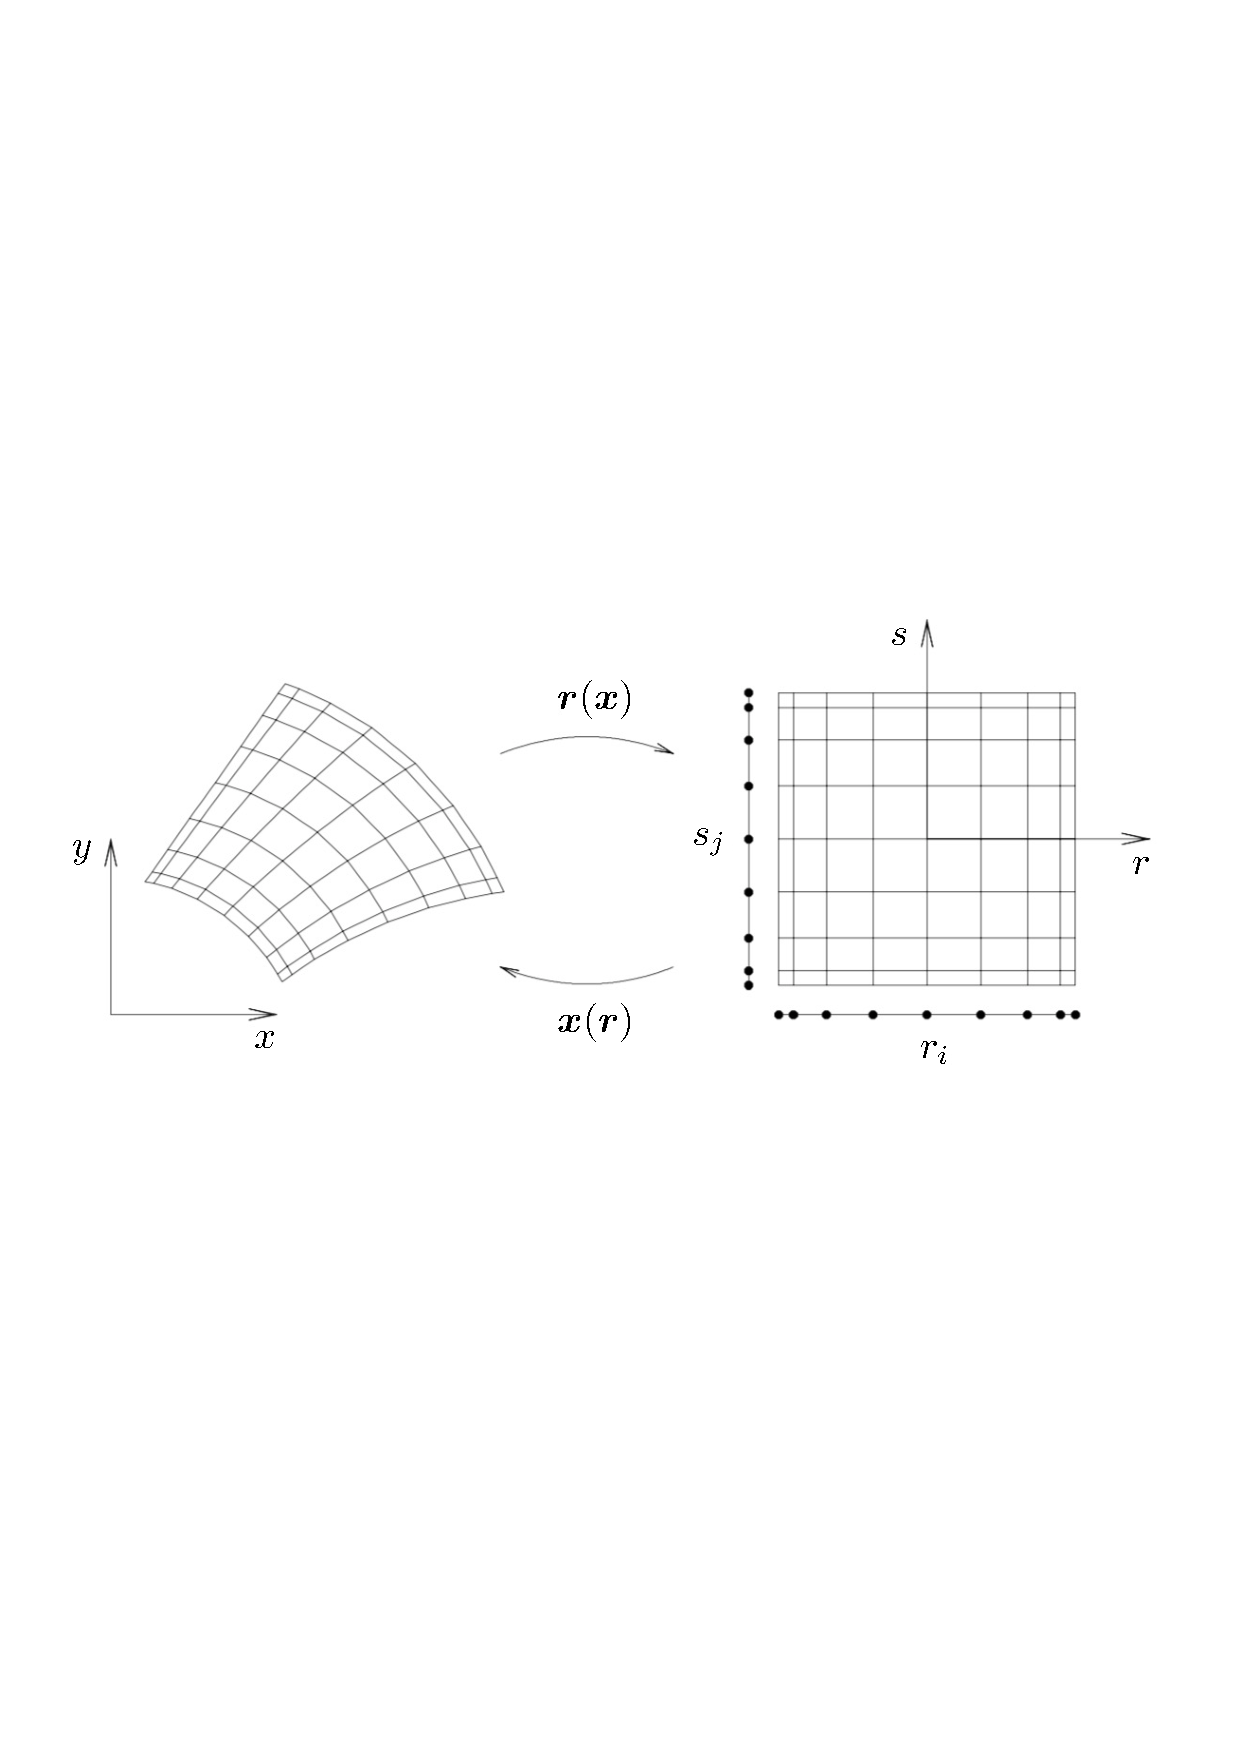
\includegraphics[width=0.65\textwidth]{xyrs}
\end{center}
\caption{Shape functions on \twod\ elements are constructed using
  tensor products of \oned\ shape functions, incorporating an
  isoparametric mapping from $(x,y)$ to master element $(r,s)$ space.
}
\label{fig.xyrs}
\end{figure}

\item[Gauss--Lobatto quadrature] Gauss--Lobatto quadrature is used for
  approximating elemental integrals: the quadrature points reside at
  the nodal points, which enables fast tensor-product techniques to be
  used for iterative matrix solution methods.  Gauss--Lobatto
  quadrature on the nodal points conveniently produces diagonal mass
  matrices when Lagrange interpolants are used as basis functions.
  
\item[Static condensation] Direct matrix solutions are sped up by
  using static condensation coupled with bandwidth reduction
  algorithms to reduce storage requirements for assembled system
  matrices.
\end{description}

While the numerical method is very accurate and efficient, it also has
the advantage that complex geometries can be accommodated by employing
unstructured conforming meshes.  The vertices of spectral elements
meshes can be produced using finite-element mesh generation
procedures, or any other method (for \Semtex, only meshes with
quadrilateral elements are accepted).

Time integration employs a backwards-time differencing scheme
described by \citet{kio91}, more recently classified as a
velocity-correction method by \citet{gush03}. One can select first,
second, or third-order time integration, but second order is usually a
reasonable compromise, and is the default scheme. Equal-order
interpolation is used for velocity and pressure
\citep[see][]{gms06}. 

As of \Semtex~V8, the `alternating skew symmetric' form \citep{zan91b}
is the default for construction of nonlinear terms in the
\NavSto\ equations (faster and just as robust as full skew symmetric,
which is still an option), and no dealiasing of product terms is
carried out for either serial or parallel operations.  As an aid to
robust operation at high Reynolds numbers, `spectral vanishing
viscosity' \citep{xupa04} can easily be enabled by setting appropriate
control tokens.
%
A significant additional novelty of \Semtex~V9.3 is the option of
robust energy-stable open boundary conditions \citep{dong15}, which
alleviate much of the numerical stability problem associated with
inflows that occur at the outflow boundary.  These also allow
ingestion of flow without causing blow-ups.
%
As of \Semtex~V9, DNS variables may optionally contain a scalar
variable in addition to velocity components and pressure.  If
requested (by running \verb|dns -f|), evolution of the scalar can be
obtained in a frozen, pre-supplied velocity field, \ie as solution of
an advection--diffusion problem.

As suggested in figure~\ref{fig.extrude}, \Semtex\ can solve problems
in \twod\ domains or in \threed\ domains that can be obtained from
arbitrary \twod\ domains by extrusion in an orthogonal direction in
which the solution fields are periodic; often such problems are
referred to as $2\,\sfrac{1}{2}$-dimensional.  Quite a large number of
fundamental problems in mechanics can be tackled using this level of
geometric complexity, but if you need genuinely \threed\ geometries
then look elsewhere.  While parallel execution is supported, the
method is only parallel across the homogeneous/extrustion/Fourier
direction, so each process has to be able to accommodate at least two
\twod\ data planes and associated overheads.  Sometimes this design
restriction is significant.  Code performance is typically quite
efficient (and fast) up to some hundreds or perhaps thousands of
processors, but this is problem-dependent.

\begin{figure}
  \begin{center}
    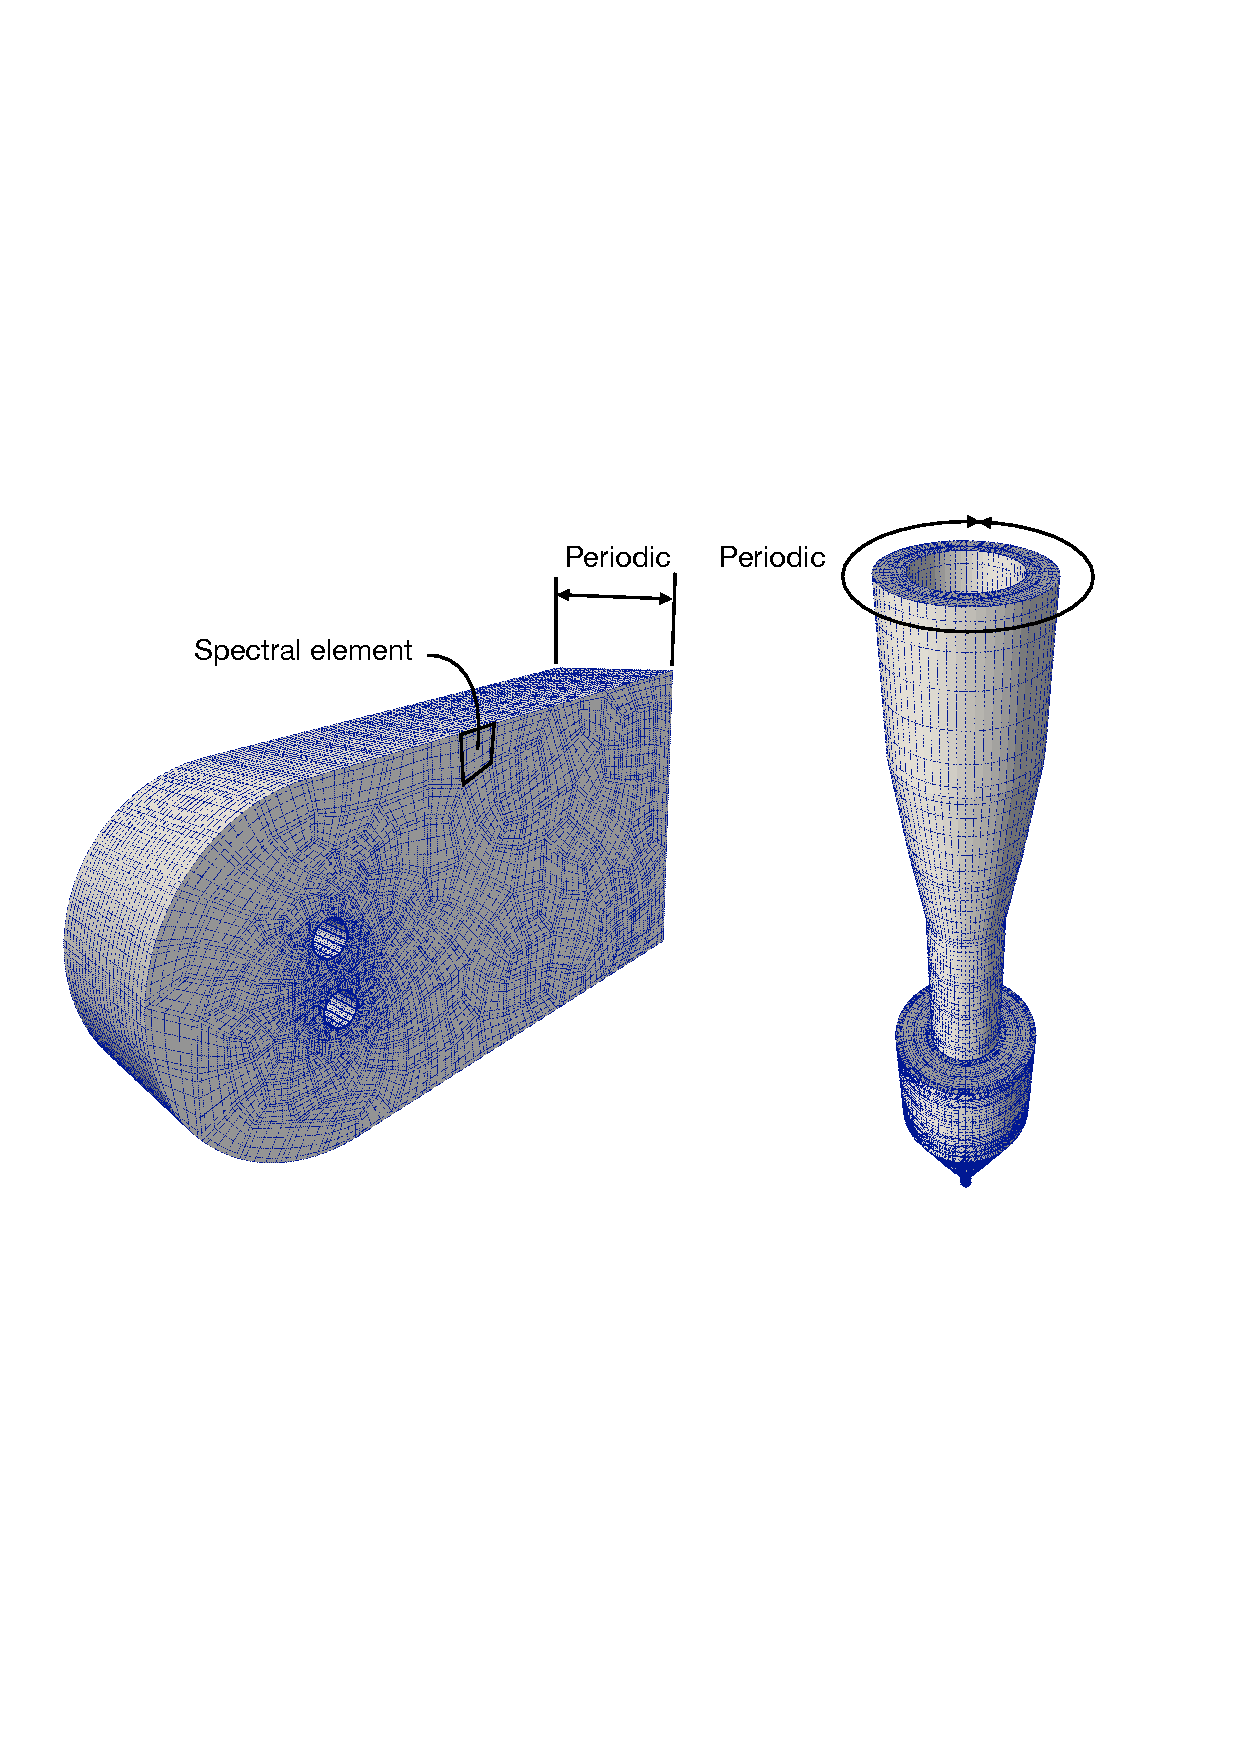
\includegraphics[width=0.85\textwidth]{2+5DSemMesh}
  \end{center}
  \caption{ \Semtex\ can solve either elliptic or incompressible
    \NavSto\ problems in domains which are either \twod\ or made
    \threed\ by extrusion of a \twod\ domain in a periodic direction.
    Either Cartesian (left) or cylindrical (right) coordinate systems
    can be used.  }
  \label{fig.extrude}
\end{figure}


%-----------------------------------------------------------------------------
\section{Implementation}

The top level of the code is written in \cpp, with calls to C and
Fortran library routines, \eg BLAS and LAPACK. The original
implementation for two-dimensional Cartesian geometries was extended
to three dimensions using Fourier expansion functions for
spatially-periodic directions in Cartesian and cylindrical spaces.
Concurrent execution is supported, using MPI as the basis for
interprocess communications, and the code has been run on a wide
variety of conventional multiprocessor machines.  Basically it ought
to work with little trouble on any contemporary Unix system.  GPUs are
not supported, nor is OpenMP.  The code is unlikely to benefit much,
if at all, from multi-threaded execution, and we generally suggest
that multi-threaded execution be disabled.

There have been various code extensions that are not part of the base
distribution. These include dynamic and non-dynamic LES
\citep{blsc03}, simple power-law type non-Newtonian rheologies
\citep{rb06}, accelerating frame of reference coupling for
aeroelasticity \citep{bh96a,bh99,bgw01,hmb03}, solution of
steady-state flows via Newton--Raphson iteration \citep{hmb02a}

However, linear stability analysis
\citep{hmb02a,bllo03b,bllo03a,bml05,shbl05,ebs06,blsh07} and optimal
transient growth analysis \citep{bbs08a} are released as an additional
open-source code base (called \Dog), with a separate user guide
called `Working \Dog'.

%-----------------------------------------------------------------------------
\section{Further reading}

The numerical techniques used by \Semtex\ are summarised in
\citet{blas19}.  A good introduction to (low-order) finite element
methods is provided by \citet{hughes87}.  The most comprehensive
references on spectral methods in general are \citet{gs77},
\citet{chqz88,chqz06}.  The first papers by \citet{pat84} and
\citet{kp86} provide a good introduction to spectral elements,
although some implementation details changed with time and
\citet{mt89} is more reflective of the methods used in \Semtex.  The
adoption of Fourier expansions to extend the method to three spatial
dimensions is discussed by \citet{ap89}, \citet{kar89} and
\citet{kar90}.  The use of spectral element techniques in cylindrical
coordinates is dealt with in \citet{blsh04}.  The book by
\citet{fun97} provides useful information and further references.
Overviews and some applications appear in \citet{kh98,hen99b}.  The
definitive reference is now the book by \citet{kars05}, but you will
also find the text by \citet*{dfm02} useful for alternative
explanations and views. More recently, the book by \citet{chqz07}
provides both theory and applications of spectral as well as spectral
element methods in fluid dynamics.

%%%%%%%%%%%%%%%%%%%%%%%%%%%%%%%%%%%%%%%%%%%%%%%%%%%%%%%%%%%%%%%%%%%%%%%%%%%%%
\chapter{Starting out}
\label{ch.start}

%============================================================================
\section{Computational environment}

It is assumed you are using some version of Unix (which includes Mac
OS~X), with a development system that includes C, \cpp\ and Fortran
compilers, bison (or yacc), make, and optionally cmake. For
post-processing, \SM\ and \Tecplot\ would be nice to have but are
not essential to get up and running, and VTK-based visualisation tools
such as \emph{VisIt} or \emph{ParaView} can alternatively be used in
place of \Tecplot.

Instructions for building and testing the codes are given in the
accompanying \texttt{StartHere.txt} and \texttt{README.md} files in
the top-level directory.  The rest of the present document assumes
that you are able to build a working set of executables and place them
in your \texttt{PATH}.

%============================================================================
\section{Equations to be solved}
\label{sec.pdes}

The central solvers provided by the \Semtex\ package are
\begin{tabbing}
\texttt{xxxxellipticx} \= \kill
\hspace*{4ex}\texttt{elliptic} \> for elliptic (Laplace, Poisson, Helmholtz)
problems,\\
\hspace*{4ex}\texttt{dns} \> for time-varying incompressible
\NavSto\ problems, with an optional scalar,
\end{tabbing}
and (if MPI is present) their equivalent multi-process versions
\texttt{elliptic\_mp} and \texttt{dns\_mp}, which can speed up
solution of \threed\ problems (see \S\,\ref{sec.mpi}).  There are also
a number of associated pre- and post-processing utilities.

Elliptic equations dealt with by \Semtex\ are in general of Helmholtz
type;
\begin{equation}
  \nabla^2 c - \lambda^2 c = f,
  \label{eq.elliptic}
\end{equation}
where $\lambda$ is a real constant and $f$ is in general a function of
space; if $\lambda=0$ we have Poisson's equation while if also $f=0$
we have Laplace's equation.  These equations are solved via a
Petrov--Galerkin method using standard finite-element techniques.
While elliptic equations may be of less interest to many readers than
the \NavSto\ equations, it is simple to provide an elliptic solver
since it underlies the time-splitting approach adopted for tackling
the \NavSto\ equations, \ie basically as a sequence of solutions to
elliptic scalar equations in each timestep.

The incompressible \NavSto\ equations are
\begin{equation}
\partial_t\bm{u}+\bm{N}(\bm{u}) = -\nabla P + \nu\nabla^2\bm{u} + \bm{f}
\quad\text{with}\quad
\bm{\nabla\cdot u} = 0;
\label{eq.navsto}
\end{equation}
$P=p/\rho$ is sometimes called the modified pressure and
$\nu=\mu/\rho$ is the kinematic viscosity, while $\bm{f}$ represents
body force per unit mass; see \S\,\ref{sec.dns_ff} for a description
of the forms of $\bm{f}$ implemented in the code.  The nonlinear terms
$\bm{N}(\bm{u})$ can be represented in two (or more) ways which are
equivalent in the continuous setting but have somewhat different
behaviour in the discrete setting: either in the `non-conservative'
form $\bm{u\cdot\nabla u}$ or the `skew-symmetric' form
$[\bm{u\cdot\nabla u} + \bm{\nabla\cdot uu}]/2$.
%
While both forms are provided, generally we use the skew-symmetric
form since compared to the non-conservative form it tends to be more
robust (has better energy conservation properties), or a
simplified/cheaper form called the `alternating skew-symmetric' which
alternates between using $\bm{u\cdot\nabla u}$ and $\bm{\nabla\cdot
  uu}$ on successive timesteps; this proves to be almost as robust as
full skew-symmetric but has a computational cost equivalent to the
non-conservative form.  We can optionally demand that $\bm{N}(\bm{u})
= 0$ in which case we have the (unsteady) Stokes equations.
%
If an advected scalar $c$ is present, the \NavSto\ equations are
augmented by the advection--diffusion equation
\begin{equation}
  \partial_t c + \bm{C}(c) = \alpha\nabla^2 c,
  \label{eq.advectdiff}
\end{equation}
where $\alpha = \nu/\Pr$ ($\Pr$ being the Prandtl number).  In this
case again, $\bm{C}(c)$ can take non-conservative form
$\bm{u\cdot\nabla}c$, skew-symmetric form $[\bm{u\cdot\nabla}c +
  \bm{\nabla\cdot u}c]/2$, the alternating equivalent or indeed
$\bm{C}(c)=0$ according to what is requested for the momentum
equations.  It is possible to run \verb|dns| in a mode which uses a
`frozen' velocity field $\bm{u}$, in which case just the
advection--diffusion equation for $c$ is integrated forward in time.

Numbers of velocity components and spatial dimensions: for
\NavSto\ type problems, \Semtex\ can solve problems which are (a)
\twod\ and \twoc, (b) \twod\ and \threec, or \threed\ and
\threec\ (a.k.a.\ 2D2C, 2D3C, 3D3C).

As with many codes used to solve the unsteady \NavSto\ equations,
diffusion-type terms (those involving $\nabla^2$) are dealt with
implicitly in time, while the nonlinear-type terms $\bm{N}$ and
$\bm{C}$ are dealt with explicitly, so that stable time integration
generally requires a time-step restriction of CFL type.

%============================================================================
\section{Mesh resolution\,---\,and design}

This is such a large area of discourse that we can't hope to
adequately cover it here; the following brief remarks are intended as
an introduction only.

Since it employs high-order finite element methods in the $(x,y)$
plane, \Semtex\ offers the choice of element-size-based refinement
(so-called $h$-refinement) or polynomial-order-based refinement
(so-called $p$-refinement) in attempting to converge a solution (it is
an $hp$-type method).  The basis polynomials share convergence
properties with (orthogonal) Legendre polynomials and the underlying
goal of mesh refinement is to achieve exponential (`spectral')
convergence of solutions with respect to polynomial order; this
typically commences when there are of order $\pi$ polynomials per
'wavelength' of solution variation \citep{gs77}.

We should point out that $p$-refinement is very straightforward in
\Semtex; different polynomial orders can be selected simply by varying
the token \verb|N_P|, the number of mesh points along the edge of
every element in the problem session file (see \eg
\S\,\ref{sec.tokens}): the \oned\ polynomial order
$p=\texttt{N\_P}-1$.
%
On the other hand, carrying out $h$-refinement will require a
completely new session file to be produced, which may imply quite a
bit more work.
%
We also note that computational work per timestep, typically dominated
by forming the nonlinear terms of the \NavSto\ equations, tends to
scale like $\texttt{N\_P}^2$ (and, of course, the number of elements).
%
Finally, \Semtex\ tends to be most efficient at moderate polynomial
orders (\eg 4 to 13); it is generally not a good idea to choose either
very low, or very high, values of $p$.

A rule-of-thumb for mesh design based on the remarks above is to aim
to have any `significant' rapid variation in solution behaviour
covered by one or two elements (the goal of $h$-refinement), and then
carry out whatever $p$-refinement is desired to get well-converged
results.
%
The path of least resistance for \twod\ mesh design is
generally to produce a session file which one guesses is quite well
resolved as far as element sizes go, then rely on converging the
solution by starting on the low end of the $p$ range and then
increasing $p$ to higher, yet moderate, values in order to commence
exponential convergence.  A few iterations of mesh design may be
required when tackling a new problem.
%

In the $z$-direction, \Semtex\ assumes the solution is periodic and
uses Fourier expansions \citep[with a 2--3--5-prime-factor
  FFT from][]{temp92}.  Choice of spanwise length scale $L_z$ is controlled
by the token \verb|BETA|, where $\beta=2\pi/L_z$, while resolution is
controlled by token \verb|N_Z|, the number of planes of real data in
the $z$ direction (the number of complex Fourier modes is then
$\texttt{N\_Z}/2$).  Convergence follows standard rules for
Fourier-spectral methods.  See \S\,\ref{sec.nz} for discussion
regarding possible values for \verb|N_Z|.

%============================================================================
\section{Files}

\Semtex\ uses a text input file which describes the mesh, boundary
conditions and other problem parameters.  We call this a session file
and typically it has no root extension.  It is written in a format
loosely patterned on HTML, which we have called FEML (for Finite
Element Markup Language) --- alternatively you could consider FEML as
a cut-down version of XML.  FEML is `just enough' to compactly
describe spectral element problems to the solvers.  There are a number
of example session files provided in the mesh subdirectory; some of
these are used in regression testing (and/or described in the
following document).  Files other than session file have standard
extensions:
\begin{tabbing}
\texttt{session.numxx} \= \kill
\texttt{session.fld}  \>
        Solution/field file.  Binary format by default,
        but with a 10-line ASCII header.\\
\texttt{session.rst}  \>
        Restart file, same format as field file.
        Read in to initialise solution if present.\\
\texttt{session.chk}  \>
        Intermediate solution checkpoint/restart files.\\
\texttt{session.avg} \> Averaged results. Read back in for
        continuation (over-written).\\
\texttt{session.his} \> History point data.\\
\texttt{session.flx} \> Time series of pressure and viscous forces
        integrated over the \texttt{wall} boundary group.\\
\texttt{session.mdl} \> Time series of kinetic energies
        in solution Fourier modes.\\
\texttt{session.par} \> Used to define initial particle locations.\\
\texttt{session.trk} \> Integrated particle locations.\\
\end{tabbing}
When writing a new session file it is prudent to run \texttt{meshpr}
(and/or \texttt{meshpr -c}) on it before trying to use it for
simulations, since \texttt{meshpr} will catch most of the
easier-to-make geometric anomalies.  You can also plot up the results
using \SM\ or other utility (such as \verb|meshplot|) as a visual
check.

NB: the 10-line ASCII header of any field-type file can quickly be viewed
using the Unix \verb|head| utility, regardless of the format of
following field data.

%============================================================================
\section{Structure of a session file}
\label{sec.session}

More details and examples for such files are provided below and in the
next chapter, but a brief outline is that a session file is an ASCII
text file with a number of sections that should each appear once, but
which can be supplied in arbitrary order.  Any line whose first
character is \verb+#+ is taken as a comment line; these can appear in
arbitrary locations within a session file.  It is generally safe to
use spaces, tabs, or new lines as white space in a session file, where
such space is permitted; within function strings to be interpreted by
the internal function parser, it is not.  In a session file, integer
indices that number specific entities such as \verb|NODES| and
\verb|ELEMENTS| are indexed starting from~1: this is also true of
related warning or error messages that \Semtex\ codes may issue,
though within the code itself, such indices are if necessary adjusted
to follow the standard C convention of being indexed starting from~0.
Much of the structure of a session file is actually free-format, but
it is generally safest to assume that collections of data which are
usually shown on a single line in the examples should not extend over
multiple lines.

As in HTML, sections are demarcated using paired opening
(\verb+<+name\verb+>+) and closing (\verb+</+name\verb+>+) tags.  The
opening tag will sometimes require a numeric attribute, \eg
\verb+<NODES NUMBER=10>+.  The minimal set of sections required for a
session file to validly describe a domain in which a solution can be
obtained is: \verb+NODES+, \verb+ELEMENTS+ and \verb+SURFACES+:
\verb+NODES+ describe the corner vertices of \verb+ELEMENTS+, while
\verb+SURFACES+ describe what happens on the outer boundaries of the
domain. Sides of all \verb+ELEMENTS+\,---\,which run between
\verb+NODES+\,---\,must either mate with the side of another
\verb+ELEMENT+ or be dealt with in the \verb+SURFACES+ section.

%----------------------------------------------------------------------------
\subsection{\texttt{NODES}}
\label{sec.nodes}

This section describes the location of the \verb|NODES| which position
\verb|ELEMENT| corner vertices in $(x,y)$ space.  The attribute
\verb|NUMBER| is required in the opening tag; this should match the
number of \verb|NODES| which follow.  This can exceed the number of
unique \verb|NODES| which are actually required for all the element
vertices, \ie spare/unused \verb|NODES| are allowed, but they have to
be included in the \verb|NUMBER| count. The minimum required
\verb|NUMBER| of \verb|NODES| is four, \ie for a single
\verb|ELEMENT|.  Each line of the \verb|NODES| section has four
entries: an integer numeric index\,---\,mostly used by human readers
of the file, since it is ignored by the code\,---\,followed by three
numbers which give the location of each \verb|NODE| in $(x,y,z)$ space
(despite the fact that only the $(x,y)$ coordinates are currently used
by \Semtex).  Different \verb|NODES| can take the same position in
$(x,y)$ space, and in fact, if you want to make a zero-width slit
boundary within a mesh, differently-indexed \verb|NODES| at identical
locations will be required.  Example, with just enough \verb|NODES|
for a single \verb|ELEMENT|:
%
{\small
\begin{verbatim}
<NODES NUMBER=4>
  1       0.0       0.0       0.0
  2       1.0       0.0       0.0
  3       0.0       1.0       0.0
  4       1.0       1.0       0.0
</NODES>
\end{verbatim}
}
%
It is often convenient to move and rescale the nodal locations
declared in this section. This may be achieved simply by setting
\verb|TOKENS| called \verb|X_SCALE|, \verb|X_SHIFT|, \verb|Y_SCALE|
and \verb|Y_SHIFT|.  The convention is that the locations are first
shifted and then scaled.

%----------------------------------------------------------------------------
\subsection{\texttt{ELEMENTS}}
\label{sec.elements}

The \verb|ELEMENTS| section also requires a \verb|NUMBER| attribute,
which gives the number of \verb|ELEMENTS| that follow.  The minimum
required \verb|NUMBER| of \verb|ELEMENTS| is one.  \Semtex\ only
presently allows quadrilateral elements, though these may have curved
edges; despite this restriction, each element is listed with an
opening \verb|<Q>| tag and a closing \verb|</Q>| tag.  The data that
describe and element are: a unique integer identifier, followed by the
opening tag \verb|<Q>|, four integer \verb|NODE| identifiers,
terminated by the closing tag \verb|</Q>|.  The ordering of these
\verb|NODES| must be such that their locations traverse a patch of
$(x,y)$ space in a counter-clockwise sense, but is otherwise
arbitrary.

The sides of an \verb|ELEMENT| are taken as running between the vertex
nodes with a 1-based indexing: the side between the first and second
\verb|NODES| is number 1, the side between the second and third
\verb|NODES| is number 2, and so on.  This information is relevant in
the following \verb|SURFACES| section. Sides of distinct elements
should of course not cross one another, though this is not actually
enforced in the code.  What \emph{is} checked is that for all
elements, each side either matches the side of another element, as
determined using the \verb|NODE| indices of all \verb|ELEMENTS|, or
has valid \verb|SURFACE| information supplied.  This ensures that the
$(x,y)$ region of a \twod\ solution domain, though possibly
multiply-connected, is completely covered by the spectral element mesh
and has appropriate boundary condition information.  A
one-\verb|ELEMENT| example based on the previous set of \verb|NODES|
follows:
%
{\small
\begin{verbatim}
<ELEMENTS NUMBER=1>
  1  <Q>  4  3  1  2  </Q>
</ELEMENTS>
\end{verbatim}
}

%----------------------------------------------------------------------------
\subsection{\texttt{SURFACES}}
\label{sec.surfaces}

Any \verb|ELEMENT| side that does not mate to the side of another
\verb|ELEMENT| based on its \verb|NODES| requires a link to boundary
condition information elsewhere in the session file or be paired up
with another element side (to provide a periodic connection).  The
\verb|SURFACES| section deals with these requirements.  Again the
opening tag must include a numeric attribute that matches the
following number of surface specifications.

Each surface is described by: a single integer index (again, mostly for
convenience of human readers), followed by a pair of integers that
give element and side numbers for this \verb|SURFACE| (these relate
back to information given in the \verb|ELEMENTS| section), and then a
tag-delimited list which provides either a single-character boundary
condition \verb|GROUP| (delimited by \verb|<B>| and \verb|</B>|) or a
pair of integers that are the element and side of a periodic
connection (delimited by \verb|<P>| and \verb|</P>|.  Note that a
periodic connection effectively deals with a pair of sides, and the
reverse connection should not also appear.  Here is an example for a
single \verb|ELEMENT| with two boundary conditions and a periodic
self-connection:
%
{\small
\begin{verbatim}
<SURFACES NUMBER=3>
  1  1  1  <B>  w  </B>
  2  1  3  <B>  t  </B>
  3  1  2  <P>  1  4  </P>
</ELEMENTS>
\end{verbatim}
}

%----------------------------------------------------------------------------
\subsection{\texttt{FIELDS}}
\label{sec.fields}


This brief section nominates the list of solution variables (\ie those
which satisfy a partial differential equation and for which we must
provide boundary conditions).  The \verb|FIELDS| are given standard
single-character name-tags: \verb|u|, \verb|v|, \verb|w| and \verb|p|
for $(x,y,z)$ velocity components and pressure, and \verb|c| for
scalar.  If we are solving an elliptic equation, only \verb|c| is
required; if solving the \NavSto\ equations, at least \verb|u|,
\verb|v| and \verb|p| must be present (for a 2D2C solution), and
\verb|c| can also appear (as a transported scalar field).  Generally,
velocity components and (optional) scalar should appear in the list
before the pressure. Example for a 2D2C flow with scalar:
%
{\small
\begin{verbatim}
<FIELDS>
  u  v  c  p
</FIELDS>
\end{verbatim}
}

%----------------------------------------------------------------------------
\subsection{\texttt{TOKENS}}
\label{sec.tokens}

In this section, \verb|TOKENS| that have significance either directly
to the solver or for use elsewhere in the session file may be defined.
This section \emph{is not} free-form: each \verb|TOKEN| must be
defined on a separate line in the form
\begin{quote}
  \verb|TOKEN = string_evaluating_to_value|
\end{quote}
The string following the equals sign should not contain white space
and may be a maximum of 2048 characters in length.  It can either
directly supply a numeric value, or be a string that may be parsed to
deliver a numeric value.  The function parser is patterned on the
\verb|hoc3| program in \citet{kernighan84} which uses \verb|yacc|, and
has many standard math functions such as $\exp$, $\cos$ and
$\tan^{-1}$ as well as standard arithmetic operations $+$, $-$, $\ast$
and $/$.  \verb|TOKENS| can be defined in terms of standard/inbuilt
\verb|TOKENS| or ones which have been defined earlier in the list.  To
see all the predefined \verb|TOKENS| and functions, check the
\Semtex\ utility \verb|"calc -h"|\,---\,\verb|calc| uses the same
parser to evaluate expressions given on the command line.

Below is a simple example in which (in order) cylindrical coordinates
are selected, the time step, \verb|D_T|, is set, as is the
time-stepping order \verb|N_TIME|, the number of points along the edge
of every element, \verb|N_P|, following which a value for a new
\verb|TOKEN|, \verb|Re|, is obtained by parsing a string and used to
set the kinematic viscosity \verb|KINVIS| as used by the \verb|dns|
solver.  (On its own, \verb|Re| is not directly significant to the
solver.) All such \verb|TOKENS| may be used subsequently in the
\verb|BCS| or \verb|FORCE| sections.
%
{\small
\begin{verbatim}
<TOKENS>
  CYLINDRICAL = 1
  D_T         = 0.001
  N_TIME      = 1
  N_P         = 7
  Re          = (30/exp(1.6))^3.
  KINVIS      = 1/Re
</TOKENS>
\end{verbatim}
}
%
This would result in the token \verb|KINVIS| taking the value
0.0450039 (to 6 sf.). Note that \verb|TOKENS| is evaluated before any
other section of a session file, so that its definitions have global
scope.

%----------------------------------------------------------------------------
\subsection{\texttt{GROUPS}}
\label{sec.groups}

This is another brief section but one that requires a numeric
parameter and which is used in defining boundary conditions. A
\verb|GROUP| associates a single-character name and a string.  The
string can potentially be used by more than a single \verb|GROUP|,
thus linking them together.  The name is also used both in the
\verb|BCS| section and the \verb|SURFACES| section, so provides a
short-hand way of linking \verb|BCS| to \verb|SURFACES|.  At first
this seems a redundant indirection; why not just have \verb|SURFACES|
and \verb|BCS|?, but it is useful because of the ability to join up
\verb|GROUPS| of \verb|BCS| via a common string, which may have
significance to the solver: \eg all \verb|BCS| in the \verb|wall|
group will have normal and tangential tractions evaluated, integrated
and printed to file \verb|session.flx|, even though the \verb|BCS|
involved may differ.
%
{\small
\begin{verbatim}
<GROUPS NUMBER=4>
  1  h  wall
  2  c  wall
  3  a  axis
  4  v  speed
</GROUPS>
\end{verbatim}
}
%
As will be elaborated in chapter~\ref{ch.examples}, the string
\verb|axis| is also significant to the solver if cylindrical
coordinates are chosen by setting \verb|CYLINDRICAL = 1| in
\verb|TOKENS|, while the string \verb|open| is required for a
\verb|GROUP| associated with a set of boundary conditions of
energy-stable open type \citep{dong15}.

%----------------------------------------------------------------------------
\subsection{\texttt{BCS}}
\label{sec.bcss}

Data in this section links a \verb|GROUP| character with a brief
description of the set of boundary conditions to be applied for
solution of each \verb|FIELD|.  Again, a \verb|NUMBER| attribute is
required in the opening tag.  For each set of \verb|BCS|, we must
supply: an integer index, a \verb|GROUP| character, and another
integer for the number of \verb|BC| descriptors that follow (which
should match the number of solution \verb|FIELDS|).  Subsequent to
that are the actual descriptors of the \verb|BCS| which are to be
applied to each \verb|FIELD| in the relevant \verb|GROUP|.  While at
first it may seem that there are apparently a variety of \verb|BC|
types which may be selected, in practice the solver is only capable of
applying either Dirichlet, Neumann or mixed (Robin) boundary
conditions for any \verb|FIELD|, but sometimes these are set
automatically within the code.  Here is an introductory example:
%
{\small
\begin{verbatim}
<BCS NUMBER=1>
  1  v  4
        <D> u = 1-exp(LAMBDA*x)*cos(2*PI*y)             </D>
        <D> v = LAMBDA/(2*PI)*exp(LAMBDA*x)*sin(2*PI*y) </D>
        <D> w = 0.0                                     </D>
        <H> p                                           </H>
</BCS>
\end{verbatim}
}
%
We see that for each \verb|FIELD| variable a boundary condition is
set.  For Dirichlet (value) boundary conditions the tag used is
\verb|<D>|; for Neumann (gradient) boundary conditions the tag is
\verb|<N>|; for mixed boundary conditions the tag is \verb|<M>|.  In
the example, Dirichlet conditions are supplied for \verb|FIELDS|
\verb|u|, \verb|v| and \verb|w|; these can either be set by parsing a
string (which should contain no white space), or directly with a
numeric value.  In the case of parsing a string, we can use
\verb|TOKENS| and/or space/time variables \verb|x|, \verb|y|, \verb|z|
and \verb|t|; the string supplied is re-parsed every timestep as the
code runs and \verb|t| updates.  We see that for the pressure,
\verb|p|, we have given the special tag \verb|<H>| to denote a
``high-order'' boundary condition, which is actually an
internally-computed Neumann type \citep[see][]{kio91}.

For more details regarding boundary condition types, see
\S\,\ref{sec.bcs} below.
%----------------------------------------------------------------------------
\subsection{\texttt{CURVES}}
\label{sec.curvess}

Element edges do not have to be straight; the user can alternatively
select circular arcs or spline fits through data supplied in external
files.  The information is supplied to the solver in the \verb|CURVES|
section.
%
{\small
\begin{verbatim}
<CURVES NUMBER=1>
  1  4  3  <ARC> 1.0 </ARC>
</CURVES>
\end{verbatim}
}
%
For each numbered \verb|CURVE| we first provide the element and side
number to which it applies (above, these numbers are 4 and 3
respectively) followed by a tagged section which nominates the kind of
curve.  For a circular \verb|ARC|, we must give the radius as a signed
number: positive values denote convex arcs while negative values
denote concave arcs.  Such curves do not have to be on the external
boundary of a mesh, but could be internal: in this case the user must
also supply corresponding information for the mating element edge.  The
code does not check that such curves conform (\eg with matching $\pm$
radii); that is up to the user.

See \S\,\ref{sec.curves} for further information relating to and a
discussion of \verb|SPLINE| curves.

%----------------------------------------------------------------------------
\subsection{\texttt{FORCE}}
\label{sec.force}

This optional section declares various kinds of body-force information
for \NavSto\ momentum equations.  Please consult \S\,\ref{sec.dns_ff}
for more detail.

%----------------------------------------------------------------------------
\subsection{\texttt{USER}}
\label{sec.user}

The principal purpose of the \verb|USER| section is in specifying
solution values which are parsed and written out as a field dump using
the \verb|compare| utility.  These could be \eg an analytical solution
or an initial condition such as a solid-body rotation.  If they are an
analytical solution, another utility (\verb|rstress|) could
subsequently be used to subtract the computed solution\,---\,this
technique is used in regression testing. Example:
%
{\small
\begin{verbatim}
<USER>
  u = -cos(PI*x)*sin(PI*y)*exp(-2.0*PI*PI*KINVIS*t)
  v =  sin(PI*x)*cos(PI*y)*exp(-2.0*PI*PI*KINVIS*t)
  p = -0.25*(cos(TWOPI*x)+cos(TWOPI*y))*exp(-4.0*PI*PI*KINVIS*t)
</USER>
\end{verbatim}
}

%----------------------------------------------------------------------------
\subsection{\texttt{HISTORY}}
\label{sec.historyy}

This section controls the output of history point data at specific
points in the domain to an ASCII file called session\verb|.his|.
Output is made every \verb|IO_HIS| integration steps.  Solution data
is written out for all \verb|FIELD| variables.  Note: the requested
point has to actually lie in the solution domain; if it does not, no
output will result. Each point has an integer numeric tag, followed by
a location in $(x,y,z)$ space (even for \twod\ solutions).
%
{\small
\begin{verbatim}
<HISTORY NUMBER=1>
  1	0.5	0.1	0.0
</HISTORY>
\end{verbatim}
}
%
While mesh nodal locations may be scaled and shifted using tokens
\verb|X_SCALE|, \verb|X_SHIFT|, \verb|Y_SCALE| and \verb|Y_SHIFT| (see
\eg \S\,\ref{sec.nodes}), the spatial locations declared in the
\verb|HISTORY| section should be given in the resulting mapped space.

%============================================================================
\section{Structure of a field file}
\label{sec.fieldfile}

Field files (with extensions \texttt{.fld}, \texttt{.rst},
\texttt{.chk}, \texttt{.avg}) have a common structure.  They all
commence with a 10-line (and 351-byte) ASCII header that briefly
describes the file content, typically followed by sequenced binary
storage of double-precision floating-point data with ordering that
matches \texttt{AuxField} structure.  It is possible to convert these
data to human-readable ASCII format, via the \texttt{convert} utility
--- and back again, if desired, to binary format --- but
\Semtex\ codes generally use the binary format for I/O of field files.
Regardless of format, one should always be able to view the contents
of the header using the Unix \texttt{head} command, which by default
reads off the first 10 lines of a file.

For example, consider the structure of a \twod\ field file; here we
will use a 2D Taylor flow, considered again later in more detail in
\S\,\ref{sec.taylor2drun}.  An example session file is supplied as
\verb|mesh/taylor2|; this has four elements, and each element has 11
collocation points on an edge (\verb|N_P=11|), so a total of 121
solution data points.  The solution is 2D2C, so the number of
$z$-planes required is \verb|N_Z=1|, but since this is a default
value, it isn't specified in the session file.  As in
\S\,\ref{sec.taylor2drun}, we will just use the \verb|compare| utility
to generate a restart file, and then look at its header. {\small
\begin{verbatim}
$ compare taylor2 > taylor2.rst
$ head taylor2.rst
taylor2                   Session
Fri Aug 18 16:08:42 2023  Created
11   11   1    4          Nr, Ns, Nz, Elements
0                         Step
0                         Time
0.02                      Time step
0.01                      Kinvis
1                         Beta
uvp                       Fields written
binary IEEE little-endian Format
\end{verbatim}
}

As previously stated, this header is 351 bytes in length, including
newline characters.  The third line of output tells us that there are
4 elements, 1 plane of data and each element is of size $N_r\times
N_s=11\times11=121$.  (In \Semtex, $N_r=N_s=\verb+N_P+$ always.)  The
ninth line of output tells us that the file contains data for the
velocity fields $u$, $v$, and pressure $p$.  That means there should
be $11\times11\times1\times4\times3=1452$ double-precision numbers in
\verb|taylor2.rst|.  Each double-precision number consumes 8 bytes,
thus we expect the size of \verb|taylor2.rst| to be
$1452\times8+351=11967$ bytes. {\small
\begin{verbatim}
$ wc -c < taylor2.rst
   11967
\end{verbatim}
}

This example is simple as there is only a single plane of data for
each field.  Each plane contains the data for its elements, written in
the order they are defined in the session file. (See \eg
figure~\ref{tay2msh}, where the elements are labelled 1\ldots4, and
the locations of the data points are also indicated for our standard
\GLL\ element mesh structure.)  The ordering of the data in each
element is row-major, starting from the bottom-left corner and working
across rows, then up, until the top-right corner is reached; this is
also the ordering in the file.\footnote{ More generally, where the
elements are distorted or rotated, from the first corner \texttt{NODE}
along the edge to the second corner \texttt{NODE}, and on up to the
third (`top-right corner') \texttt{NODE} location for any quadratic
\texttt{ELEMENT} in a session file.}  Following the data for the first
field ($u$), here a single plane of storage, we would find the data
for the second field, then the third (and so on, if there were more
fields indicated in the header).  The extension to files with more
planes of data is simple: the planes are written in order for the
first field, then the second, etc.

Binary data in \threed\ field files (where $\verb|N_Z|>1$) by default
have physical-space ordering, even though most \threed\ calculations
in \Semtex\ are carried out after a Fourier transformation in the $z$
coordinate.  If you wish to get the data to a Fourier-transformed
state (say, to extract a particular \twod\ Fourier mode), use the
\texttt{transform} utility; see \eg \S\S\,\ref{sec.transform}
and~\ref{sec.xplane}.  The ordering of data planes following
real--complex transformation matches how they are stored in
\verb|AuxField|s: the $0$th Fourier mode, which is the $z$-average at
each $(x,y)$ location and real, is stored as the first plane of data,
while the $\verb|N_Z|/2$th, `Nyquist', or `oddball' mode, also real,
is stored as the second plane (typically, this will be set to zero
since we do not evolve Nyquist modes).  After these two planes of data
we have the real and imaginary planes of each complex Fourier mode, in
order, up to $(\verb|N_Z|/2)-1$.

Sometimes, field files will hold more than a single set of data for a
complete field (\eg a sequence of field dumps).  In this case, each
set of data commences with a new header (each with a different
\texttt{Time}).  To find out how many dumps are in a file, you could
do something like: {\small
\begin{verbatim}
$ convert taylor.rst | grep Session | wc -l
   1
\end{verbatim}
}


%============================================================================
\section{Utilities}
\label{sec.utilities}

(See also the more extensive discourse of chapter~\ref{ch.utilities}.)
Source code for these tools is found in the \texttt{utility}
directory.  Here is a summary of the most-used utilities:
\begin{tabbing}
\texttt{enumeratexx}  \= \kill
\texttt{addfield} \> 
        Compute and add vorticity vector components, divergence, etc., to
        a field file.\\
\texttt{addquick} \> 
        An example shell script for adding arbitrary but simple fields
        of your choice using\\
        \> UNIX \verb|sed| and \verb|awk| utilities together with
        \verb|chop| and \verb|convert|. (Quick \emph{and dirty}!)\\
\texttt{calc} \>      
        A simple calculator that calls \verb+femlib+'s function
        parser. The inbuilt parser functions\\ \>and default \texttt{TOKENS}
        can be seen if you run \texttt{calc -h}.\\
\texttt{compare} \>   
        Generate restart files, compare solutions to a function.\\
\texttt{convert} \>   
        Convert field file formats (IEEE-big/little, to/from ASCII).\\
\texttt{eneq} \>   
        Compute terms in the energy transport equation.\\
\texttt{assembly}  \>
        Generate global node numbering used in matrix assembly.  \\
        \> The output of this utility is no longer directly used by
        simulation codes \\ 
        \> (since they now generate assembly mappings at runtime), \\
        \> but is supplied for checking purposes.  It replaces the \\
        \> former utility called \verb+enumerate+.\\
\texttt{integral} \>
        Obtain the 2D integral of fields over the
        domain area.\\
\texttt{interp} \>   
       Interpolate a field file onto a (2D) set of points.\\
\texttt{meshplot} \>
        Generate a PostScript plot of mesh from \texttt{meshpr} output.\\
\texttt{meshpr} \>    
        Generate 2D mesh locations for plotting or checking.\\
\texttt{noiz} \>      
        Add a Gaussian-distributed random perturbation to a field file.\\
\texttt{probe} \>   
        Probe a field file at a set of 2D/3D points. Different
        interfaces to \texttt{probe}\\ \> are obtained through the names
        \texttt{probeline} and \texttt{probeplane}: \\ \> make these soft
        links by hand.\\
\texttt{project} \>   
        Convert a field file to a different order interpolation.\\
\texttt{rectmesh} \>
        Generate a template session file for a rectangular domain.\\
%\texttt{resubmit} \> Shell utility for automatic job resubmission.\\
\texttt{rstress} \>
	Postprocess to compute Reynolds stresses from a file of
        time-averaged variables.\\
%\texttt{save} \> Shell utility for automatic job resubmission.\\
\texttt{sem2tec} \>   
        Convert field files to AMTEC \Tecplot\ format.
        Note that by default, \verb|sem2tec| \\
        \> interpolates the
        original GLL-mesh-based data onto 
        a (isoparametrically mapped) \\ \> uniform mesh for improved visual 
        appearance.  Sometimes it is useful  to see the \\ \> original data 
        (and mesh); for this use the \verb+-n 0+ command-line
        argument to \verb+sem2tec+.\\
\texttt{sem2vtk} \>   
        Convert field files to VTK format (\emph{VisIt, ParaView}).\\
\texttt{transform} \>      
        Take Fourier, Legendre, modal basis transform of a field
	file. Invertible.\\
\texttt{wallmesh} \>      
        Extract the mesh nodes corresponding to surfaces with the
	\verb+wall+ group.
\end{tabbing}




%%%%%%%%%%%%%%%%%%%%%%%%%%%%%%%%%%%%%%%%%%%%%%%%%%%%%%%%%%%%%%%%%%%%%%%%%%%%%
\chapter{Example applications}
\label{ch.examples}

We will run through some examples to illustrate input files, utility
routines, and use of the solvers.  While most users will likely be
primarily interested in solving \NavSto\ problems, we commence by
outlining the use of the elliptic solver.

%============================================================================
\section{Elliptic equations}
\label{sec.laplace}

The elliptic solver can be used to solve Laplace, Poisson or Helmholtz
problems in \twod\ and \threed\ Cartesian and cylindrical coordinate
systems, vide \eqref{eq.elliptic}.  From a code development viewpoint
it also provides a means to test new formulations of elliptic solution
routines which are used in the \NavSto\ type solvers; historically,
\verb|elliptic| was written and tested prior to \verb|dns|.
%
In this section we illustrate the use of the elliptic solver for a \twod\
Laplace problem, $\nabla^2 c = 0$.  In this case the function
\begin{equation}
  c(x,y) = \sin(x) \exp(-y)
\end{equation}
satisfies Laplace's equation and is used to set the boundary
conditions.  This example illustrates the methods used to set BCs and
also to generate curved element boundaries.  Also we will demonstrate
the selection of the iterative PCG solver \citep{barrett94} as an
alternative to the default direct Cholesky solver
\citep{anderson99}. The session file \texttt{laplace7} shown below is
provided in the \verb|mesh| subdirectory.
%
{\small
\begin{verbatim}
##############################################################################
# Laplace problem on unit square, BC c(x, y) = sin(x)*exp(-y)
# is also the analytical solution.  Use essential (Dirichlet) BC
# on upper, curved edge, with natural (Neumann) BCs elsewhere.

<FIELDS>
  c
</FIELDS>

<USER>  
        Exact sin(x)*exp(-y)
        c =   sin(x)*exp(-y)
</USER>

<TOKENS>
        N_P      = 11
        TOL_REL  = 1e-12
        STEP_MAX = 1000
</TOKENS>

<GROUPS NUMBER=4>
        1       d       value
        2       a       slope
        3       b       slope
        4       c       slope
</GROUPS>

<BCS NUMBER=4>
        1       d       1
                        <D>     c =  sin(x)*exp(-y)     </D>
        2       a       1
                        <N>     c = -cos(x)*exp(-y)     </N>
        3       b       1
                        <N>     c =  cos(x)*exp(-y)     </N>
        4       c       1
                        <N>     c =  sin(x)*exp(-y)     </N>
</BCS>

<NODES NUMBER=9>
        1       0.0     0.0     0.0
        2       0.5     0.0     0.0
        3       1.0     0.0     0.0
        4       0.0     0.5     0.0
        5       0.5     0.5     0.0
        6       1.0     0.5     0.0
        7       0.0     1.0     0.0
        8       0.5     1.0     0.0
        9       1.0     1.0     0.0
</NODES>

<ELEMENTS NUMBER=4>
        1       <Q>  1  2  5  4  </Q>
        2       <Q>  2  3  6  5  </Q>
        3       <Q>  4  5  8  7  </Q>
        4       <Q>  5  6  9  8  </Q>
</ELEMENTS>

<SURFACES NUMBER=8>
        1       1       1       <B>     c       </B>
        2       2       1       <B>     c       </B>
        3       2       2       <B>     b       </B>
        4       4       2       <B>     b       </B>
        5       4       3       <B>     d       </B>
        6       3       3       <B>     d       </B>
        7       3       4       <B>     a       </B>
        8       1       4       <B>     a       </B>
</SURFACES>

<CURVES NUMBER=1>
        1       4       3       <ARC>   1.0     </ARC>
</CURVES>
\end{verbatim}
}

Refer to \S\,\ref{sec.session} for a discussion of the purposes of
each of the sections within this file.  Within the \verb|TOKENS|
section, \verb|N_P=11| declares that there will be 11 points along the
side of each element and hence, \twod\ element shape functions are
tensor products of 10th-order polynomials.  \verb|TOL_REL=1e-12|
directs the iterative preconditioned conjugate gradient solver, if
used, to stop when the solution residual $||r^{(i)}|| = ||A x^{(i)} -
b|| < \verb|TOL_REL|\times||b||$, while \verb|STEP_MAX=1000| directs that
no more than 1000 iterations be taken in striving to reach
\verb|TOL_REL|; note that these values are only relevant if an
iterative solver is chosen instead of default direct solution, and
that the default values of the two tokens are respectively \verb|1e-8|
and \verb|500|, as may be established by running \verb|calc -h|.

%----------------------------------------------------------------------------
\subsection{Curved element edges (and plotting the mesh)}
\label{sec.curves}

The mesh for this problem consists of a set of four elements, one of
which, the 3rd edge of element~4, specified in the \texttt{CURVES}
section, is a a circular arc.  Both \texttt{ARC} and \texttt{SPLINE}
type curves are currently implemented.  For the \texttt{ARC} type, the
parameter supplies the radius of the curve: a positive value implies
that the curve makes the element convex on that side, while a negative
value implies a concave side.  Note that where elements mate along a
curved side, the curve must be defined twice, once for each element,
and with radii of different signs on each side.  The mesh for this
problem can be seen in figure~\ref{lapcurve}; mesh output is generated
by running the \verb|meshpr| utility, from which a PostScript file may
be generated and visualised using the \verb|meshplot| utility.
%
{\small
\begin{verbatim}
$ meshpr laplace7 | meshplot -i -n -o mesh.ps -d gv
\end{verbatim}
} \noindent If you have the \verb|gv| utility installed (for X11
display of PostScript) you should see a plot like
figure~\ref{lapcurve}.  Alternatively you could (again, assuming you
have an appropriate utility installed) convert the output to PDF, \eg
%
{\small
\begin{verbatim}
$ meshpr laplace7 | meshplot -i -n | ps2pdf - > laplace7.pdf
\end{verbatim}
}
\begin{figure}
\begin{center}
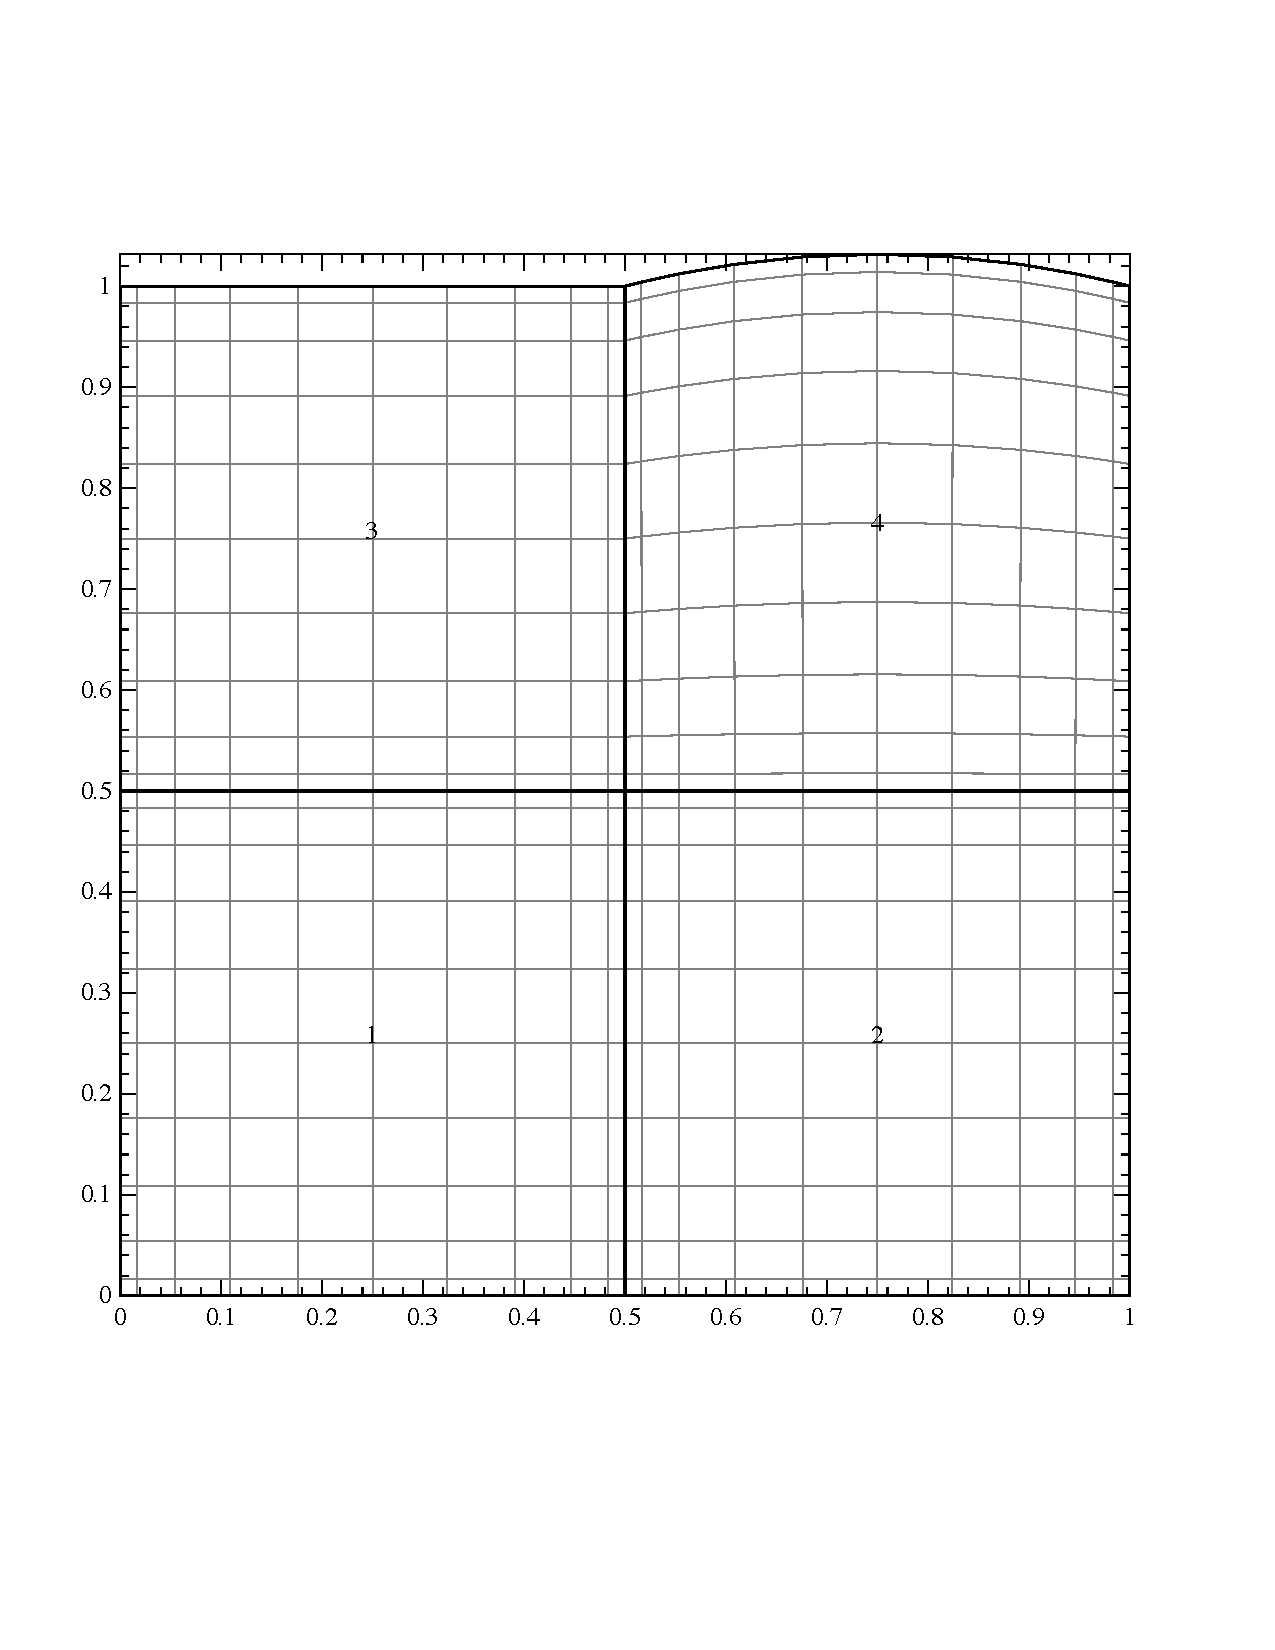
\includegraphics[width=0.5\textwidth]{laplace6}
\end{center}
\caption{
\label{lapcurve}
  The mesh corresponding to the \texttt{laplace7} session file.  Note
  that the number of points along the edge of every element is
  \texttt{N\_P = 11} as declared in the \texttt{TOKENS} section and
  that internal points are placed inside non-rectangular elements, \eg
  element 4, using isoparametric mapping. This image was produced
  using the \texttt{meshplot} utility.}
\end{figure}

For the \texttt{SPLINE} type, the parameter supplies the name of an
ASCII file which contains a list of ($x$,\,$y$) coordinate pairs
(white-space delimited). Naturally, the list of points should be in
arc-length order. A single file can be used to supply the curved edges
for a set of element edges. The vertices of the relevant elements do
not have to lie exactly on the splined curve\,---\,if they do not,
those vertices get shifted to the intersection of the projection of
the straight line joining the original vertex position and its
neighbouring `curve-normal' vertex, and the cubic spline joining the
points in the file. On the other hand, it is good practice to ensure
that the declared vertex locations lie close to the spline, and to
visually check the mesh that is produced.

%----------------------------------------------------------------------------
\subsection{Boundary conditions}

The sections \texttt{GROUPS} and \texttt{BCS} are used to specify
boundary conditions for the problem.  The \texttt{GROUPS} section
associates a character group tag (\eg \verb+d+) with a string (\eg
\verb+value+), but note that different groups can be associated with
the same string\footnote{This allows actions to be taken over a set of
  BCs which share the same string.}.  Groups \verb+a+, \verb+b+ and
\verb+c+ will be used to set natural (\ie slope or Neumann), boundary
conditions ($\partial c/\partial n=\textrm{value}$), while group
\verb+a+ will be used to impose an essential or Dirichlet condition
($c=\textrm{value}$).

The \texttt{BCS} section is used to define the boundary conditions
which will be applied for each group.  For each group, after the
numeric tag (ignored) appears the character for that group, then the
number of BCs that will be applied: this corresponds to the number of
fields in the problem, in this case~1 (\verb+c+).  BCs are typically
of Dirichlet, Neumann, or Robin/mixed type (note that domain
periodicity can be employed but that this does not constitute a
boundary condition).  So in this case we will declare the BC types to
be \verb+D+ ({\texttt D}irichlet) for group \verb+d+ and \verb+N+
({\texttt N}eumann) for groups \verb+a+, \verb+b+ and \verb+c+.  On
Neumann boundaries, the value which must be supplied is the slope of
the solution along the outward normal to the solution domain.  Note
the fact that the BCs can be set using the function parser, using the
built-in functions and variables, also any symbols defined in the
\texttt{TOKENS} section, as well as the spatial variables \verb+x+,
\verb+y+ and \verb+z+.  The BCs can also be functions of time,
\verb+t+, and for time-varying problems, which this is not, the
boundary conditions are re-evaluated every time step.

The BC groups are associated with element edges in the
\texttt{SURFACES} section.  Periodic edges, Dirichlet, Neumann and
mixed boundary conditions can be arbitrarily combined in a problem.
Dirichlet conditions over-ride Neumann ones where they meet (say at
the corner node of an element). See further discussion on boundary
conditions in \S\,\ref{sec.bcs} below.

%----------------------------------------------------------------------------
\subsection{Running the codes}
\label{sec.runell}

We will run the \verb|elliptic| solver and compare the computed
solution to the analytical solution.  We will first run with the
default direct solver: 
%
{\small
\begin{verbatim}
$ elliptic laplace7
-- Forcing                 : set to zero
-- Initial condition       : set to zero
-- Installing matrices for field 'c' [*]
-- REMARK: Field: 'c' error norms (inf, L2, H1): 8.54872e-15  2.15768e-15  5.46269e-14
\end{verbatim}
}
%Field: 'c' error norms (inf, L2, H1): 5.44009e-15  1.5745e-15  6.77144e-14

The `\verb|Installing matrices|' message indicates that a direct
solution will be carried out.  Next try the iterative (PCG) solver
using the \verb+-i+ command-line option to \texttt{elliptic}:
%
{\small
\begin{verbatim}
$ elliptic -i laplace7
-- Forcing                 : set to zero
-- Initial condition       : set to zero
-- REMARK: Field: 'c' error norms (inf, L2, H1): 8.32201e-13  2.93711e-13  5.01449e-12
\end{verbatim}
}
%Field: 'c' error norms (inf, L2, H1): 1.93215e-12  8.91558e-13  1.88887e-11
\noindent
In this case the direct solver is more accurate, but comparable
accuracy with the iterative solver could be obtained by decreasing
\verb+TOL_REL+ in the \texttt{TOKENS} section (and if necessary by
further increasing \verb+STEP_MAX+).

For post-processing we can prepare a \Tecplot\ input file (which can
also be read by \emph{VisIt} and \emph{Paraview})
%
{\small
\begin{verbatim}
$ meshpr laplace7 | sem2tec laplace7.fld
\end{verbatim}
}
%
\noindent
which produces \verb|laplace7.plt|, an input file format which can be
read by \Tecplot.  A contour plot of the solution obtained with
\Tecplot\ is shown in figure~\ref{fig.lapcont}.

\begin{figure}
\begin{center}
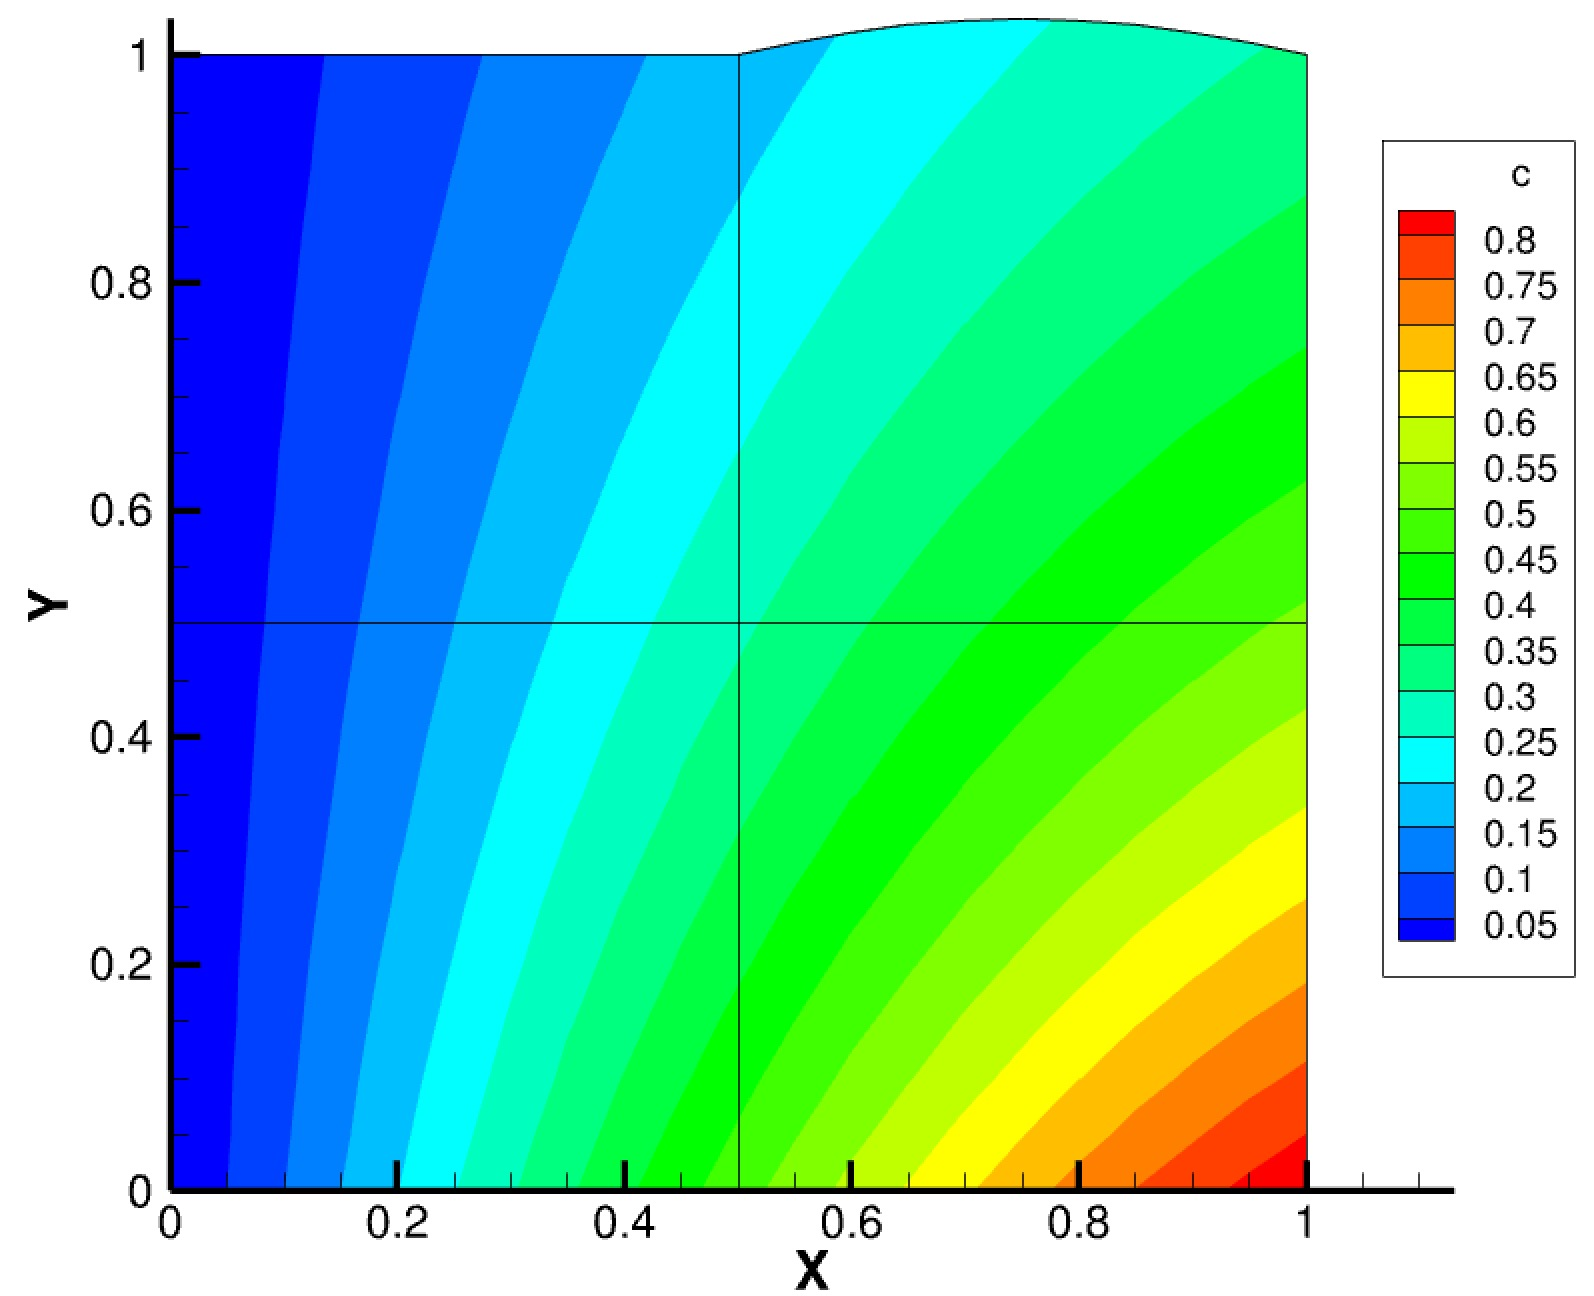
\includegraphics[width=0.55\textwidth]{laplace6cont}
\end{center}
\caption{ Solution corresponding to the \texttt{laplace7} session
  file.  This image was produced using \Tecplot.  }
\label{fig.lapcont}
\end{figure}

%----------------------------------------------------------------------------
\subsection{Laplace, Poisson, Helmholtz problems}

Poisson and Helmholtz problems differ from Laplace problems in that
they have a forcing term.  For elliptic problems this is supplied in
the \verb|USER| section by a line of the type \verb|Forcing <string>|
where \verb|<string>| is ASCII text without white space which can be
parsed, \eg either a numeric constant or a function of spatial
variables can be supplied.  In the case of Helmholtz problems we need
also to supply a positive numerical value for the token
\verb|LAMBDA2|, equivalent to the constant $\lambda^2$.

If one has an analytical solution to the problem in question, this can
also be supplied in the \verb|USER| section with a line of the type
\verb|Exact <string>| where again \verb|<string>| is ASCII text which
can be parsed.  The outcomes are compared to the computed numerical
solutions and various error norms are reported, as we saw in
\S\,\ref{sec.runell}.  An analytical solution isn't required to run
the solver, so this line is optional.

Various session files for elliptic problems can be found in the
\verb|mesh| subdirectory, with fairly obvious names. One of these,
\verb|laplace8| is for a \threed\ problem in cylindrical coordinates.
If a solution is desired in cylindrical coordinates, one must also set
the token \verb|CYLINDRICAL=1|; this convention applies in general for
\Semtex\ codes such as \verb|dns| and the utility programs too.  The
default value of \verb|CYLINDRICAL| is 0 (corresponding to Cartesian
coordinates).


%============================================================================
\section{2D Taylor flow}
\label{sec.taylor}

Taylor flow is an analytical solution to the \NavSto\ equations.
In the $x$--$y$ plane the solution is 
\begin{eqnarray}
        u &=& -\cos(\pi x) \sin(\pi y) \exp(-2\pi^2\nu t),\\
        v &=& +\sin(\pi x) \cos(\pi y) \exp(-2\pi^2\nu t),\\
        p &=& -(\cos(2\pi x) + \cos(2\pi y)) \exp(-4\pi^2\nu t)/4
            + \textrm{const}.
\end{eqnarray}
The solution is doubly periodic in space, with periodic length 2.
Since the solution is periodic in both directions, no boundary
conditions are required but the periodicity must be specified in the
\verb|SURFACES| section.  As usual for \NavSto\ solutions, the
pressure can only be specified up to an arbitrary constant.  An
interesting feature of this solution is that the nonlinear and
pressure gradient terms balance one another, leaving a diffusive decay
of the initial condition\,---\,this property is occasionally useful for
checking codes.

%----------------------------------------------------------------------------
\subsection{Session file}

Below is the complete input or \emph{session} file we will use; it has
four elements, each of the same size, with 11 nodes along each edge.
This session file, \texttt{taylor2}, is supplied in the \verb|mesh|
subdirectory.
%
{\small
\begin{verbatim}
##############################################################################
# 2D Taylor flow in the x--y plane has the exact solution
#
#       u = -cos(PI*x)*sin(PI*y)*exp(-2.0*PI*PI*KINVIS*t)
#       v =  sin(PI*x)*cos(PI*y)*exp(-2.0*PI*PI*KINVIS*t)
#       w =  0
#       p = -0.25*(cos(2.0*PI*x)+cos(2.0*PI*y))*exp(-4.0*PI*PI*KINVIS*t)
#
# Use periodic boundaries (no BCs).

<USER>
        u = -cos(PI*x)*sin(PI*y)*exp(-2.0*PI*PI*KINVIS*t)
        v =  sin(PI*x)*cos(PI*y)*exp(-2.0*PI*PI*KINVIS*t)
        p = -0.25*(cos(TWOPI*x)+cos(TWOPI*y))*exp(-4.0*PI*PI*KINVIS*t)
</USER>

<FIELDS>
        u v p
</FIELDS>

<TOKENS>
        N_TIME  = 2
        N_P     = 11
        N_STEP  = 20
        D_T     = 0.02
        Re      = 100.0
        KINVIS  = 1.0/Re
        TOL_REL = 1e-12
</TOKENS>

<NODES NUMBER=9>
        1       0.0       0.0       0.0
        2       1.0       0.0       0.0
        3       2.0       0.0       0.0
        4       0.0       1.0       0.0
        5       1.0       1.0       0.0
        6       2.0       1.0       0.0
        7       0.0       2.0       0.0
        8       1.0       2.0       0.0
        9       2.0       2.0       0.0
</NODES>

<ELEMENTS NUMBER=4>
        1 <Q> 1 2 5 4 </Q>
        2 <Q> 2 3 6 5 </Q>
        3 <Q> 4 5 8 7 </Q>
        4 <Q> 5 6 9 8 </Q>
</ELEMENTS>

<SURFACES NUMBER=4>
        1       1       1       <P>     3       3       </P>
        2       2       1       <P>     4       3       </P>
        3       2       2       <P>     1       4       </P>
        4       4       2       <P>     3       4       </P>
</SURFACES>
\end{verbatim}
}

(Below we give a brief reprise of some information we earlier dealt
with in \S\,\ref{sec.session}.)

The first section of the file in this case contains comments; a line
anywhere in the session file which starts with a \verb+#+ is
considered to be a comment.  Following that are a number of sections
which are opened and closed with matching keywords in HTML style (e.g.
\verb+<USER>+--\verb+<\USER>+).  Keywords are not case sensitive.
The complete list of keywords is: \texttt{TOKENS}, \texttt{FIELDS}, 
\texttt{GROUPS}, \texttt{BCS}, \texttt{NODES}, \texttt{ELEMENTS}, 
\texttt{SURFACES}, \texttt{CURVES} and \texttt{USER}.  Depending on the
problem being solved, some sections may not be needed, but the minimal
set is: \texttt{FIELDS}, \texttt{NODES}, \texttt{ELEMENTS} and
\texttt{SURFACES}.  Anywhere there is likely to be a long list of
inputs within the sections, the \texttt{NUMBER} of inputs is also
required; this currently applies to \texttt{GROUPS}, \texttt{BCS},
\texttt{NODES}, \texttt{ELEMENTS}, \texttt{SURFACES} and
\texttt{CURVES}.  In each of these cases the numeric tag appears first for
each input, which is free-format.  The order in which the sections
appear in the session file is irrelevant.

The \texttt{USER} section is ignored by the solvers, and is used
instead by utilities --- in this case it will be used by the
\texttt{compare} utility both to generate the initial condition or
\emph{restart} file and to check the computed solution.  This
section declares the variables corresponding to the solution fields
with the corresponding analytical solutions.  The variables
\texttt{x}, \texttt{y}, \texttt{z} and \texttt{t} can be used to
represent the three spatial coordinates and time.  Note that some
constants such as \texttt{PI} and \texttt{TWOPI} are predefined, while
others, like \texttt{KINVIS}, are set in the \texttt{TOKENS} section.
Note also the use of predefined functions, accessed through an inbuilt
function parser.\footnote{The built-in functions and predefined constants
can be found by running \texttt{calc -h}.}

The \texttt{FIELDS} section declares the one-character names of
solution fields.  The names are significant: \texttt{u}, \texttt{v}
and \texttt{w} are the three velocity components (we only use
\texttt{u} and \texttt{v} here for a 2D solution and the \texttt{w}
component is always the direction of Fourier expansions), \texttt{p}
is the pressure field.  The field name \texttt{c} is also recognised
as a scalar field for certain solvers, e.g. the elliptic solver.

In the \texttt{TOKENS} section, second-order accurate time integration
is selected (\verb+N_TIME = 2+) and the number of Lagrange knot points
along the side of each element is set to 11 (\verb+N_P = 11+),
corresponding to the use of 10th-order polynomials, and giving
\twod\ elemental shape functions which are tensor-products of
10th-order Lagrange polynomials.\footnote{The minimum accepted value of
\texttt{N\_P = 2},
  corresponding to
  (bi)linear shape functions.  The practicable upper value is around 20.}
The code will integrate for 20 timesteps (\verb+N_STEP = 20+) with a
timestep of 0.02 (\verb+D_T = 0.002+).  The kinematic viscosity is set
as the inverse of the Reynolds number (100): note the use of the
function parser here.  Finally the relative tolerance used as a
stopping test in the PCG iteration used to solve the viscous substep
on the first timestep is set as $1.0\times10^{-12}$.

The shape of the mesh is defined by the \texttt{NODES} and
\texttt{ELEMENTS} sections.  Here there are four elements, each
obtained by connecting the corner nodes in a counterclockwise
traverse.  The $x$, $y$ and $z$ locations of the nodes are given, and
the four numbers given for the nodes of each element are indices
within the list of nodes.

In the final section (\texttt{SURFACES}), we describe how the edges of
elements which define the boundary of the solution domain are dealt
with.  In this example, the solution domain is periodic and there are
no boundary conditions to be applied, so the \texttt{SURFACES} section
describes only periodic (\verb+P+) connections between elements.  For
example, on the first line, side~1 of element~1 is declared to be
periodic with side~3 of element~3 --- side~1 runs between the first
and second nodes, while side~3 runs between the third and fourth.

%----------------------------------------------------------------------------
\subsection{Running the codes}
\label{sec.taylor2drun}

Assume we're in the \texttt{dns} directory of the distribution, that
the \texttt{compare}, \texttt{meshpr} and
\texttt{sem2tec} utilities have been compiled, as well as the
\texttt{dns} simulation code.
{\small
\begin{verbatim}
$ cp ../mesh/taylor2 .
\end{verbatim}
}

First we'll examine the mesh, in this case using \SM\ macros supplied with the
\Semtex\ distribution as an alternative to using the \verb|meshplot|
utility.
%
{\small
\begin{verbatim}
$ meshpr taylor2 > taylor2.msh
$ sm
Hello Hugh, please give me a command
: meshplot taylor2.msh 1
Read lines 1 to 1 from taylor2.msh
Read lines 2 to 485 from taylor2.msh
: meshnum
: meshbox
: quit
\end{verbatim}
}
\noindent
You should have seen a plot like that in figure~\ref{tay2msh}. (Note:
while you are building up the mesh parts of a session file, perhaps by
hand, you may use \texttt{meshpr -c} to suppress some of the checking
for matching element edges and curved boundaries that \texttt{meshpr}
does by default.)
\begin{figure}
\begin{center}
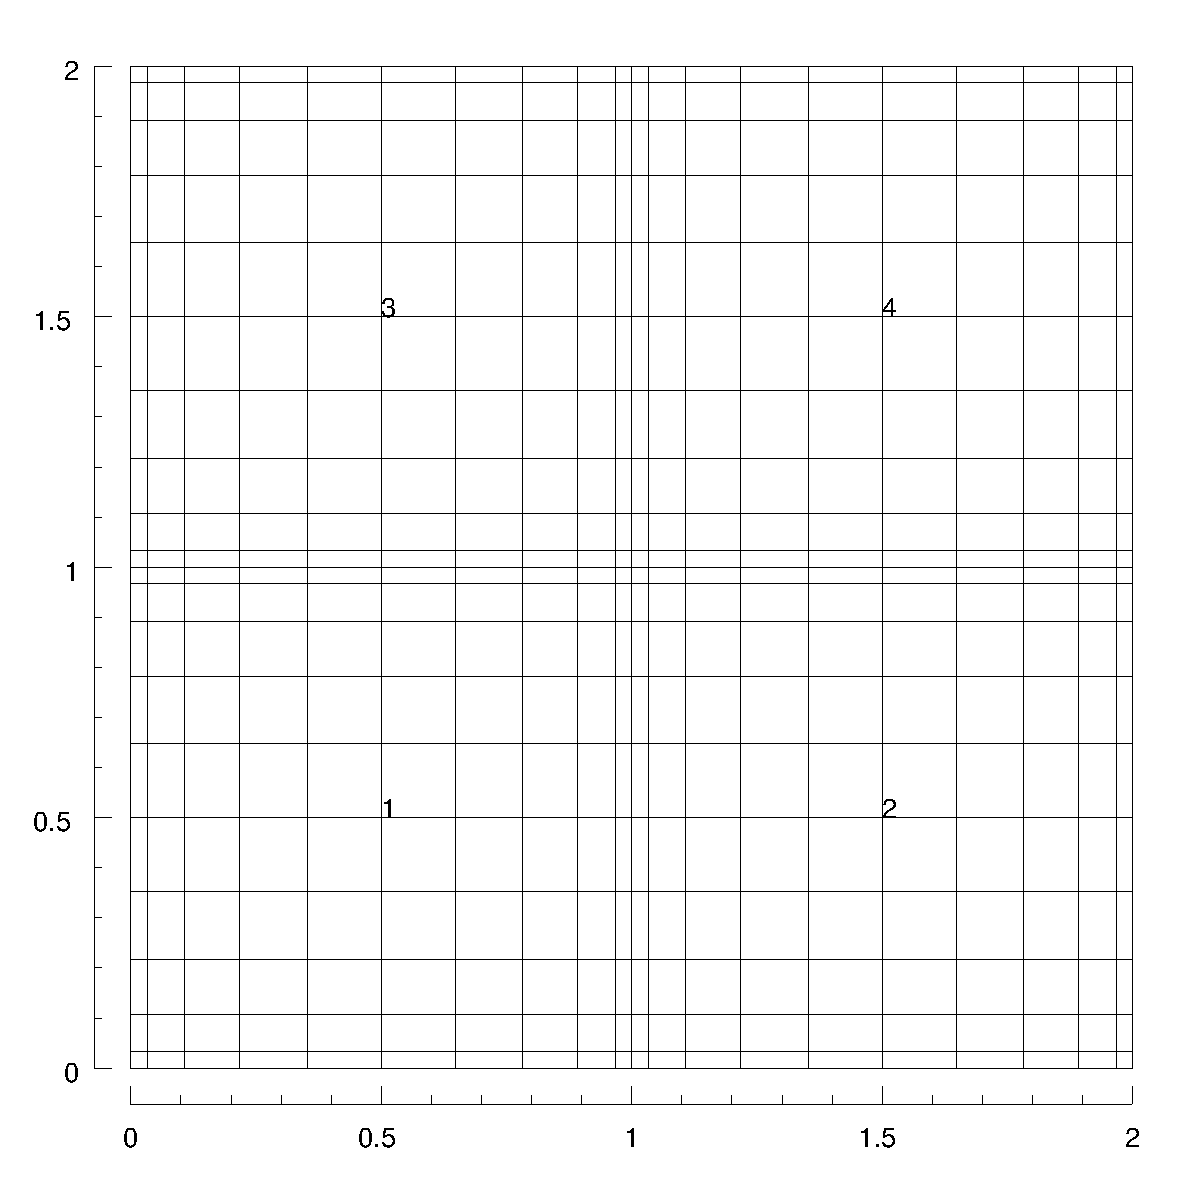
\includegraphics[width=0.5\textwidth]{taylor2mesh}
\end{center}
\caption{
\label{tay2msh}
  The mesh corresponding to the \texttt{taylor2} session file.  This
  image was produced by using \SM\ macros.  }
\end{figure}

The \texttt{compare} utility is used to generate a file of initial
conditions using information in the \verb|USER| section of a session
file.  This \emph{restart} file contains binary data, but we'll have a
look at the start of it by converting it to ASCII format.  Also, the
header of these files is always in ASCII format, and so can be
examined directly using the Unix \texttt{head} command.  {\small
\begin{verbatim}
$ compare taylor2 > taylor2.rst
$ convert taylor2.rst | head -20
taylor2                   Session
Wed Aug 13 21:39:47 1997  Created
11   11   1    4          Nr, Ns, Nz, Elements
0                         Step
0                         Time
0.02                      Time step
0.01                      Kinvis
1                         Beta
uvp                       Fields written
ASCII                     Format
     0.000000000      0.000000000    -0.5000000000 
     0.000000000     0.1034847104    -0.4946454574 
     0.000000000     0.3321033052    -0.4448536974 
     0.000000000     0.6310660897    -0.3008777952 
     0.000000000     0.8940117093    -0.1003715318 
     0.000000000      1.000000000      0.000000000 
     0.000000000     0.8940117093    -0.1003715318 
     0.000000000     0.6310660897    -0.3008777952 
     0.000000000     0.3321033052    -0.4448536974 
     0.000000000     0.1034847104    -0.4946454574 
\end{verbatim}
}

Then the \texttt{dns} solver is run to generate a solution or
\emph{field} file, \texttt{taylor2.fld}.  This has the same format
as the restart file.
{\small
\begin{verbatim}
$ dns taylor2
-- Initial condition       : read from file taylor2.rst
-- Coordinate system       : Cartesian
   Solution fields         : uvp
   Number of elements      : 4
   Number of planes        : 1
   Number of processors    : 1
   Polynomial order (np-1) : 10
   Time integration order  : 2
   Start time              : 0
   Finish time             : 0.4
   Time step               : 0.02
   Number of steps         : 20
   Dump interval (steps)   : 20 (checkpoint)
-- Installing matrices for field 'u' [*]
-- Installing matrices for field 'v' [.]
-- Installing matrices for field 'p' [*]
Step: 1  Time: 0.02
Step: 2  Time: 0.04
Step: 3  Time: 0.06
Step: 4  Time: 0.08
Step: 5  Time: 0.1
Step: 6  Time: 0.12
Step: 7  Time: 0.14
Step: 8  Time: 0.16
Step: 9  Time: 0.18
Step: 10  Time: 0.2
Step: 11  Time: 0.22
Step: 12  Time: 0.24
Step: 13  Time: 0.26
Step: 14  Time: 0.28
Step: 15  Time: 0.3
Step: 16  Time: 0.32
Step: 17  Time: 0.34
Step: 18  Time: 0.36
Step: 19  Time: 0.38
Step: 20  Time: 0.4
\end{verbatim}
}

Note the difference in the information following the three
`\verb|Installing matrices|' messages: every instance of `\verb|*|'
indicates a new matrix system is being computed, while a `\verb|.|'
indicates that a previously computed system will be used: in this
case, the matrix system for `\verb|v|' can re-use the matrix system
for `\verb|u|', since the Helmholtz constant and boundary conditions
match.

We can use \texttt{compare} to examine how close the solution is to the
analytical solution.  The output of \texttt{compare} in this case
is a field file which contains the difference: since we're only interested
in seeing error norms here, we'll discard this field file.
{\small
\begin{verbatim}
$ compare taylor2 taylor2.fld > /dev/null
Field 'u': norm_inf: 1.127e-05
Field 'v': norm_inf: 1.127e-05
Field 'p': norm_inf: 4.224e-01
\end{verbatim}
}
\noindent
The velocity error norms are small, as expected, but the pressure norm
will always be arbitrary, corresponding to the fact that the pressure
can only be specified to within an arbitrary constant\,---\,hence the
reported errors for pressure may be quite large, but this isn't a
cause for alarm.

Finally we will use \texttt{sem2tec} to generate a \Tecplot\ input
file.  The \Tecplot\ utility \texttt{preplot} must also be in your
\texttt{path}; source for this code is supplied in the \verb|utility|
subdirectory.  {\small
\begin{verbatim}
$ sem2tec -m taylor2.msh taylor2.fld
\end{verbatim}
}
\noindent
This produces \texttt{taylor2.plt} which can be used as input to
\Tecplot.  The plot in figure~\ref{tay2soln} was generated using
\Tecplot\ and shows pressure contours and velocity vectors.  Notice
that largely for cosmetic reasons, by default \texttt{sem2tec}
interpolates the results from the Gauss--Lobatto--Legendre grid (seen
in figure~\ref{tay2msh}) used in the computation to a uniformly-spaced
grid of the same order (use \verb|-n 0| to defeat this feature and
see the actual solution values and on the original mesh).

\begin{figure}
\begin{center}
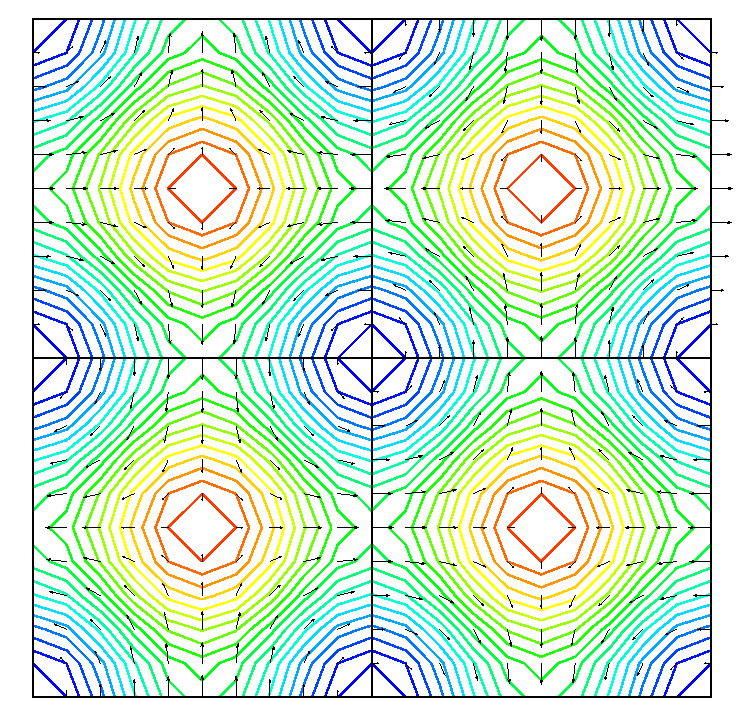
\includegraphics[width=0.5\textwidth]{taylor2}
\end{center}
\caption{
\label{tay2soln}
  Solution to the \texttt{taylor2} problem, visualized using \Tecplot.
}
\end{figure}

%============================================================================
\section{3D Kovasznay flow}
\label{sec.kovas}

Here we will solve another viscous flow for which an analytical
solution exists, the Kovasznay flow (we will call the session file
\verb+kovas3+).  In the $(x,y)$ plane, this flow is
\begin{eqnarray}
        u &=& 1 - \exp(\lambda x)\cos(2\pi y)           \\
        v &=& \lambda/(2\pi)\exp(\lambda x)\sin(2\pi y) \\
        w &=& 0                                         \\
        p &=& (1 - \exp(\lambda x))/2  + \textrm{const}. 
\end{eqnarray}
where $\lambda = \Rey/2 - (0.25\Rey^2 + 4\pi^2)^{1/2}$.

Although the solution has only two velocity components, we will set up
and solve the problem in three dimensions, with a periodic length in
the~$z$ direction of~1.0 and eight $z$-planes of data.  The length in
the $z$ direction is set within the code by the variable \verb+BETA+
where $\beta=2\pi/L_z$.  The default value of \verb+BETA+ is 1, so we
reset this in the \texttt{TOKENS} section using the function parser.
The exact velocity boundary conditions are supplied on at the left and
right edges of the domain, and periodic boundaries are used on the
upper and lower edges (the domain has $-0.5\le y\le0.5$).  Since the
flow evolves to a steady state, first order timestepping is employed
(\verb+N_TIME = 1+).

The session file below is provided
as \verb|mesh/kovas3|.

{\small
\begin{verbatim}
##############################################################################
# Kovasznay flow in the x--y plane has the exact solution
#
#       u = 1 - exp(lambda*x)*cos(2*PI*y)
#       v = lambda/(2*PI)*exp(lambda*x)*sin(2*PI*y)
#       w = 0
#       p = (1 - exp(lambda*x))/2
#
# where lambda = Re/2 - sqrt(0.25*Re*Re + 4*PI*PI).
#
# This 3D version uses symmetry planes on the upper and lower boundaries
# with flow in the x-y plane.
#
# Solution accuracy is independent of N_Z since all flow is in the x--y plane.

<USER>
        u = 1.0-exp(LAMBDA*x)*cos(TWOPI*y)
        v = LAMBDA/(TWOPI)*exp(LAMBDA*x)*sin(TWOPI*y)
        w = 0.0
        p = 0.5*(1.0-exp(LAMBDA*x))
</USER>

<FIELDS>
        u v w p
</FIELDS>

<TOKENS>
        N_Z    = 8
        N_TIME = 1
        N_P    = 8
        N_STEP = 500
        D_T    = 0.008
        Re     = 40.0
        KINVIS = 1.0/Re
        LAMBDA = Re/2.0-sqrt(0.25*Re*Re+4.0*PI*PI)
        Lz     = 1.0
        BETA   = TWOPI/Lz
</TOKENS>

<GROUPS NUMBER=1>
        1       v       velocity
</GROUPS>

<BCS NUMBER=1>
        1       v       4
                        <D> u = 1-exp(LAMBDA*x)*cos(2*PI*y)             </D>
                        <D> v = LAMBDA/(2*PI)*exp(LAMBDA*x)*sin(2*PI*y) </D>
                        <D> w = 0.0                                     </D>
                        <H> p                                           </H>
</BCS>

<NODES NUMBER=9>
        1      -0.5    -0.5     0.0
        2       0      -0.5     0.0
        3       1      -0.5     0.0
        4      -0.5     0       0.0
        5       0       0       0.0
        6       1       0       0.0
        7      -0.5     0.5     0.0
        8       0       0.5     0.0
        9       1       0.5     0.0
</NODES>

<ELEMENTS NUMBER=4>
        1 <Q> 1 2 5 4 </Q>
        2 <Q> 2 3 6 5 </Q>
        3 <Q> 4 5 8 7 </Q>
        4 <Q> 5 6 9 8 </Q>
</ELEMENTS>

<SURFACES NUMBER=6>
        1       1       1       <P>     3       3       </P>
        2       2       1       <P>     4       3       </P>
        3       2       2       <B>     v               </B>
        4       4       2       <B>     v               </B>
        5       3       4       <B>     v               </B>
        6       1       4       <B>     v               </B>
</SURFACES>
\end{verbatim}
}

%----------------------------------------------------------------------------
\subsection{`High-order' pressure boundary condition}

Note that there is only one boundary group, and four boundary
conditions must be set, corresponding to the four fields \verb+u+,
\verb+v+, \verb+w+ and \verb+p+.  A new feature is a pressure BC of
type \verb+H+, which is an internally-computed Neumann boundary
condition, (a \verb+H+igh-order pressure BC) as described in
\citet{kio91}.  This is the kind of pressure BC that we would
typically supply on all surfaces except on outflow boundaries or, in
cylindrical coordinates, on the $x$-axis.  The pressure BC is computed
internally, so no value is required (if given, it will be ignored).

%----------------------------------------------------------------------------
\subsection{Running the codes}

Since we already have an analytical solution for the problem, we may
as well use that to generate an initial condition and then run for a
moderate number of time steps (\eg 200) to see if the discrete
solution diverges much from this.
{\small
\begin{verbatim}
$ compare kovas3 > kovas3.rst
$ dns kovas3
\end{verbatim}
}

After running \verb+dns+, we confirm there is only a single dump in
the field file \verb+kovas3.fld+,\footnote{Note the use of
  \texttt{convert} and \texttt{grep} to see how many dumps are
  contained within a field file.  More generally (\eg within a script)
  we could pipe the outcome into \texttt{wc -l} to provide a numeric
  value.}  then run compare in order to examine the error norms for
the solution.
%
{\small
\begin{verbatim}
$ convert kovas3.fld | grep -i session
kovas3                    Session
$ compare kovas3 kovas3.fld > /dev/null
Field 'u': norm_inf: 5.773e-05
Field 'v': norm_inf: 3.145e-05
Field 'w': norm_inf: 0.000e+00
Field 'p': norm_inf: 9.350e-01
$ meshpr kovas3 | sem2tec -n20 kovas3.fld
\end{verbatim}
}
%
The errors incurred are relatively small and could be reduced by
re-running with increased polynomial order; in \verb|kovas3|,
\verb|N_P = 8|, \ie the polynomial order in each direction for each
element is~7.  Increasing \verb|N_P| to~13 will reduce the errors in
velocity by more than three orders of magnitude (check for yourself),
illustrating the exponential convergence property of spectral element
methods.

Finally we prepare input for \Tecplot, projecting the
interpolation to a $20\times20$ grid in each element in order to
produce smoother contours.  A view of the result can be seen in
figure~\ref{kov3soln}.
\begin{figure}
\begin{center}
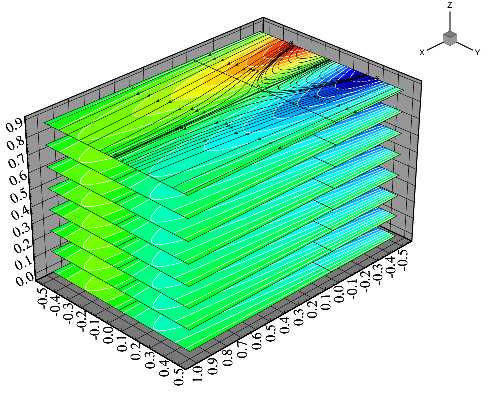
\includegraphics[width=0.65\textwidth]{kovas3_bitmap}
\end{center}
\caption{
\label{kov3soln}
  Solution to the \texttt{kovas3} problem, visualised using \Tecplot.
  The plot shows contours of $v$ velocity component and streamlines.
  Since the solution is in fact \twod\ but we carried out a
  \threed\ solution, the results are identical on each $z$-plane of
  data. }
\end{figure}

%----------------------------------------------------------------------------
\subsection{Valid values of \texttt{N\_Z} in \Semtex}
\label{sec.nz}

This was a `fake' \threed\ problem since while we used \verb|N_Z=8|,
in fact the solution is \twod, at least in Cartesian coordinates; the
solution is invariant in the $z$-direction (in
chapter\,\ref{ch.dns101} we will examine turbulent DNS which \emph{is}
\threed). However, in passing, we note here the values which
\verb|N_Z| can take for \threed\ solutions: since we use a 2--3--5
prime-factor complex--complex FFT \citep{temp92} together with a
real--complex conversion \citep[\eg \S\,12.3,][]{press92} to carry out
Fourier transforms, \verb|N_Z| must be even (factorisable by 2) but
can also have factors of 3 and 5.  Hence valid values of \verb|N_Z|
are: $2, 4, 6, 8, 10, 12, 16, 20, 24, 30, 32 \ldots$.  Of course
\verb|N_Z=1| is also valid but the solution will perforce be \twod.
However, owing to the use of complex--real conversion in which the
Nyquist data are always set to zero, in fact a solution with
\verb|N_Z=2| will also always be \twod\ (the same on both $z$-planes).
Hence the minimum value of \verb|N_Z| which in fact allows any
\threed\-ity in \Semtex\ is 4.  For \NavSto\ problems, flows which
have $\texttt{N\_Z}>1$ must also have three velocity components.

%============================================================================
\section{Vortex breakdown\,---\,a cylindrical-coordinate problem}
\label{sec.vb}

Here we will examine a problem which uses the cylindrical coordinate
option of \verb+dns+.  The physical situation is a cylindrical cavity,
$H/R=2.5$ with the flow driven by a spinning lid at one end.  At the
Reynolds number we'll use, $\Rey=\Omega R^2/\nu=2119$, a vortex
breakdown is known to occur.  The flow in this case is invariant in
the azimuthal direction, but has three velocity components (it is
2D3C) and hence we use \verb|N_Z=1|.  In the cylindrical code, the
order of spatial directions and velocity components is $x$, $r$,
$\theta$, though we retain the coordinate names $x$, $y$, $z$ (\ie
$y\equiv r$ and $z\equiv\theta$, $v\equiv\bm{u}_r$,
$w\equiv\bm{u}_\theta$).

Note that for a full circle in the azimuthal direction, \texttt{BETA =
  1.0}, which is the default value. In fact, the value would not be
used in the present solution, since all derivatives in the azimuthal
direction are implicitly zero when \verb+N_Z=1+. (But see
\S\,\ref{sec.cbcs} below.)  The session file below is provided as
\verb|mesh/vb1|.

{\small
\begin{verbatim}
#############################################################################
# 15 element driven cavity flow.  2D/3C

<FIELDS>
        u v w p
</FIELDS>

<TOKENS>
        CYLINDRICAL = 1
        N_Z         = 1
        BETA        = 1.0
        N_TIME      = 2
        N_P         = 11
        N_STEP      = 100000
        D_T         = 0.01
        Re          = 2119
        KINVIS      = 1/Re
        OMEGA       = 1.0
        TOL_REL     = 1e-12
</TOKENS>

<GROUPS NUMBER=3>
        1       v       velocity
        2       w       wall
        3       a       axis
</GROUPS>

<BCS NUMBER=3>
        1       v       4
                        <D>     u = 0           </D>
                        <D>     v = 0           </D>
                        <D>     w = OMEGA*y     </D>
                        <H>     p               </H>
        2       w       4
                        <D>     u = 0           </D>
                        <D>     v = 0           </D>
                        <D>     w = 0           </D>
                        <H>     p               </H>
        3       a       4
                        <A>     u               </A>
                        <A>     v               </A>
                        <A>     w               </A>
                        <A>     p               </A>
</BCS>

<NODES NUMBER=24>
        1       0       0       0
        2       0.4     0       0
        3       0.8     0       0
        4       1.5     0       0
        5       2.4     0       0
        6       2.5     0       0
        7       0       0.15    0
        8       0.4     0.15    0
        9       0.8     0.15    0
        10      1.5     0.15    0
        11      2.4     0.15    0
        12      2.5     0.15    0
        13      0       0.75    0
        14      0.4     0.75    0
        15      0.8     0.75    0
        16      1.5     0.818   0
        17      2.4     0.9     0
        18      2.5     0.9     0
        19      0       1       0
        20      0.4     1       0
        21      0.8     1       0
        22      1.5     1       0
        23      2.4     1       0
        24      2.5     1       0
</NODES>

<ELEMENTS NUMBER=15>
        1       <Q>      1  2  8  7     </Q>
        2       <Q>      2  3  9  8     </Q>
        3       <Q>      3  4 10  9     </Q>
        4       <Q>      4  5 11 10     </Q>
        5       <Q>      5  6 12 11     </Q>
        6       <Q>      7  8 14 13     </Q>
        7       <Q>      8  9 15 14     </Q>
        8       <Q>      9 10 16 15     </Q>
        9       <Q>     10 11 17 16     </Q>
        10      <Q>     11 12 18 17     </Q>
        11      <Q>     13 14 20 19     </Q>
        12      <Q>     14 15 21 20     </Q>
        13      <Q>     15 16 22 21     </Q>
        14      <Q>     16 17 23 22     </Q>
        15      <Q>     17 18 24 23     </Q>
</ELEMENTS>

<SURFACES NUMBER=16>
        1       1       1       <B>     a       </B>
        2       2       1       <B>     a       </B>
        3       3       1       <B>     a       </B>
        4       4       1       <B>     a       </B>
        5       5       1       <B>     a       </B>
        6       5       2       <B>     v       </B>
        7       10      2       <B>     v       </B>
        8       15      2       <B>     v       </B>
        9       15      3       <B>     w       </B>
        10      14      3       <B>     w       </B>
        11      13      3       <B>     w       </B>
        12      12      3       <B>     w       </B>
        13      11      3       <B>     w       </B>
        14      11      4       <B>     w       </B>
        15      6       4       <B>     w       </B>
        16      1       4       <B>     w       </B>
</SURFACES>
\end{verbatim}
}

The mesh for the problem is shown in figure~\ref{vb1msh}, and the
velocity field estimate obtained by running \verb|dns| is shown
compared to an experimental streakline flow visualisation on the front
cover of this document.
\begin{figure}
\begin{center}
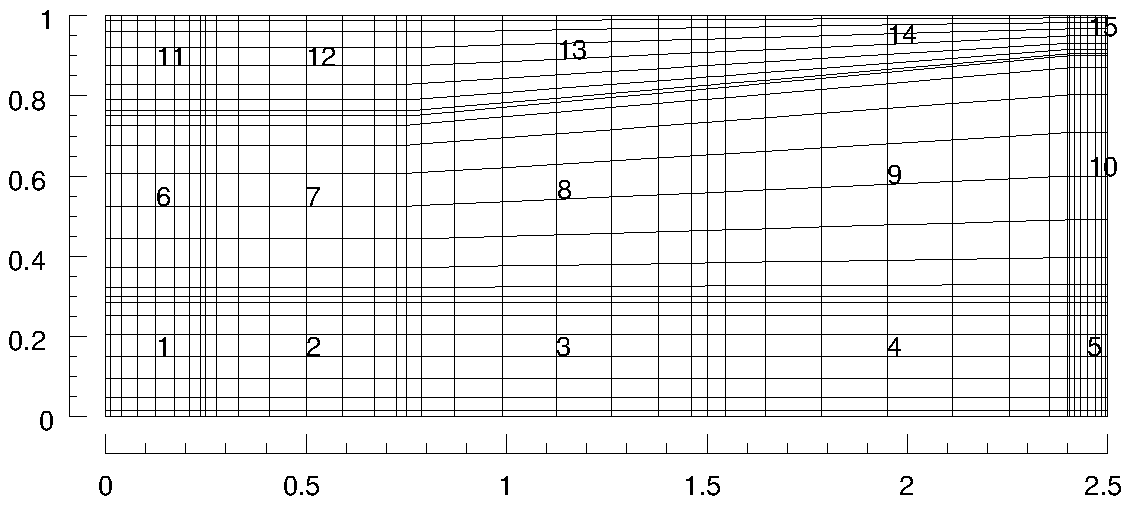
\includegraphics[width=0.6\textwidth]{vb1mesh}
\end{center}
\caption{
\label{vb1msh}
  Mesh for the vortex breakdown problem.  The spinning lid is at
  right.  This image was produced using \SM\ macros.  }
\end{figure}

%----------------------------------------------------------------------------
\subsection{BCs for cylindrical coordinates}
\label{sec.cbcs}

A new feature here is the use of BCs of type \verb+A+ on the axis of
the flow.  Internally, the code sets the BC there either as zero
essential or zero natural, depending on the physical variable and the
Fourier mode.  Owing to the coupling scheme used in the code
\citep{blsh04}, the boundary conditions for the radial and azimuthal
velocities \verb+v+ and \verb+w+ must be of the same type within each
group.  A further restriction is that the group to which the axis
belongs must have name \verb+axis+.

Finally, say you wish to solve a cylindrical-coordinate problem where
you know that, while the solution may be \threed, there is an $n$-fold
azimuthal symmetry (say $n=3$). In that case, it is much cheaper to
solve with \verb+BETA=3+, and use one-third the number of azimuthal
planes that would be required for \verb+BETA=1+.  One does not have to
change the specification of axis boundary conditions when making such
a change, as they are internally computed according to Fourier mode
index and \verb|BETA|.

%============================================================================
\section{Buoyancy driven flow in a cavity}
\label{sec.tdrivcav}

Next we will examine a \NavSto\ problem with an advected scalar
(temperature) and Boussinesq buoyancy (see \S\,\ref{sec.bous}) driving
flow in a rectangular cavity.  The session file shown below is
provided as \verb|tdrivcav1|.
%
{\small
\begin{verbatim}
# Thermal driven cavity problem for buoyancy-driven flow.
# Left edge is hot, right edge is cool, top and bottom are insulated.

<FIELDS>
        u v c p
</FIELDS>

<USER>
        u = 0.0
        v = 0.0
        c = T_MAX-x
        p = 0.0
</USER>

<FORCE>
        BOUSSINESQ_TREF    = 0.0
        BOUSSINESQ_BETAT   = RAYLEIGH*PRANDTL
        BOUSSINESQ_GRAVITY = 1.0
        BOUSSINESQ_GY      = -1.0
</FORCE>

<TOKENS>
        N_TIME   = 1
        N_P      = 10
        N_STEP   = 5000
        IO_FLD   = 1000
        D_T      = 0.0008
        T_MAX    = 1.0
        T_MIN    = 0.0
        PRANDTL  = 0.71
        RAYLEIGH = 1.0e4
        KINVIS   = PRANDTL
</TOKENS>

<GROUPS NUMBER=3>
        1       h       hot
        2       c       cold
        3       i       insulated
</GROUPS>

<BCS NUMBER=3>
        1       h       4
                        <D>     u = 0.0         </D>
                        <D>     v = 0.0         </D>
                        <D>     c = T_MAX       </D>
                        <H>     p               </H>
        2       c       4
                        <D>     u = 0.0         </D>
                        <D>     v = 0.0         </D>
                        <D>     c = T_MIN       </D>
                        <H>     p               </H>
        3       i       4
                        <D>     u = 0.0         </D>
                        <D>     v = 0.0         </D>
                        <N>     c = 0.0         </N>
                        <H>     p               </H>
</BCS>

<NODES NUMBER=9>
        1       0.0     0.0     0.0
        2       0.5     0.0     0.0
        3       1.0     0.0     0.0
        4       0.0     0.5     0.0
        5       0.5     0.5     0.0
        6       1.0     0.5     0.0
        7       0.0     1.0     0.0
        8       0.5     1.0     0.0
        9       1.0     1.0     0.0
</NODES>

<ELEMENTS NUMBER=4>
        1       <Q>     1 2 5 4         </Q>
        2       <Q>     2 3 6 5         </Q>
        3       <Q>     4 5 8 7         </Q>
        4       <Q>     5 6 9 8         </Q>
</ELEMENTS>

<SURFACES NUMBER=8>
        1       1       1       <B>     i       </B>
        2       2       1       <B>     i       </B>
        3       2       2       <B>     c       </B>
        4       4       2       <B>     c       </B>
        5       4       3       <B>     i       </B>
        6       3       3       <B>     i       </B>
        7       3       4       <B>     h       </B>
        8       1       4       <B>     h       </B>
</SURFACES>
\end{verbatim}
}
%
{\small
\begin{verbatim}
$ dns tdrivcav1
-- Initial condition       : set to zero
-- Coordinate system       : Cartesian
   Solution fields         : uvcp
   Number of elements      : 4
   Number of planes        : 1
   Number of processors    : 1
   Polynomial order (np-1) : 9
   Time integration order  : 1
   Start time              : 0
   Finish time             : 4
   Time step               : 0.0008
   Number of steps         : 5000
   Dump interval (steps)   : 1000 (checkpoint)
-- Installing matrices for field 'u' [*]
-- Installing matrices for field 'v' [.]
-- Installing matrices for field 'c' [*]
-- Installing matrices for field 'p' [*]
Step: 1  Time: 0.0008
Step: 2  Time: 0.0016
Step: 3  Time: 0.0024
Step: 4  Time: 0.0032
Step: 5  Time: 0.004
...
...
Step: 4996  Time: 3.9968
Step: 4997  Time: 3.9976
Step: 4998  Time: 3.9984
Step: 4999  Time: 3.9992
Step: 5000  Time: 4
# CFL: 1.4, dt (max): 0.000572, dt (set): 0.0008 (139%), field: v, elmt: 1
# Divergence Energy:    0.000283
\end{verbatim}
}

By now the structure of the session file should be fairly familiar,
except perhaps for the specification of a thermally driven buoyancy
body force in the \verb|FORCE| section, for which you are referred
ahead to read \S\,\ref{sec.dns_ff} and \S\,\ref{sec.bous} in
particular.  Note how variables are set to achieve a desired Rayleigh
number
$\Ra=\cg\beta_TL^3
(T_\textrm{max}-T_\textrm{min})/(\nu\alpha T_\textrm{ref})=1\times10^4$.

% ----------------------------------------------------------------------------
\section{Timestepping stability: CFL and divergence energy}
\label{sec.cfl}

We have not yet touched upon the \verb|dns| output information
regarding CFL (Courant--Friedrichs--Lewy) limits and divergence (as
listed in the example above).  These are reported in \verb|dns| output
every \verb|IO_CFL| steps.  The CFL estimates are computed according
to methods outlined in \S\,6.3 of \citet{kars05} based on velocity
component values and mesh sizes, and are roughly proportional to
$u\Delta t/\Delta x$.  Typically, we need to keep CFL values below
around unity to maintain stability with explicit time integration
methods of the kind used here for advection based on nonlinear terms.
We see that at the end of integration, our CFL value is actually
larger than this (1.4), though stable integration is achieved (partly
since, as we are integrating towards a steady-state solution, we have
used first-order timestepping rather than the second-order default).
Also, we see which velocity component ($v$) is the most critical with
respect to CFL instability, and in which element (1) this occurs.

On the lines following CFL estimate reports, we get another indication
of solution robustness, the (average) divergence energy, which is
$(2A)^{-1}\int (\bm{\nabla\cdot u})^2\, \cd \Omega$ where
$A=\int\cd\Omega$ is the area of the domain.  Our numerical method,
which uses a time-splitting approach to integrating the
\NavSto\ equations, commits a divergence error that is asymptotically
proportional to $|\Delta t|^\texttt{N\_TIME}$ (even when the mesh is
adequate for spatial resolution). If the timestep is too large, we
will also get large divergence energy: for solutions with length and
velocity scales of order unity, a rule of thumb is that reported
divergence energies should be well below unity in order for results to
be reasonably well resolved in time.  Typically, if the timestep is
too large, CFL instability will set in and both the reported CFL and
divergence energy values will start to become very large before the
simulation terminates with a floating-point overflow error (Unix
\verb|SIG8|).

\begin{figure}
\begin{center}
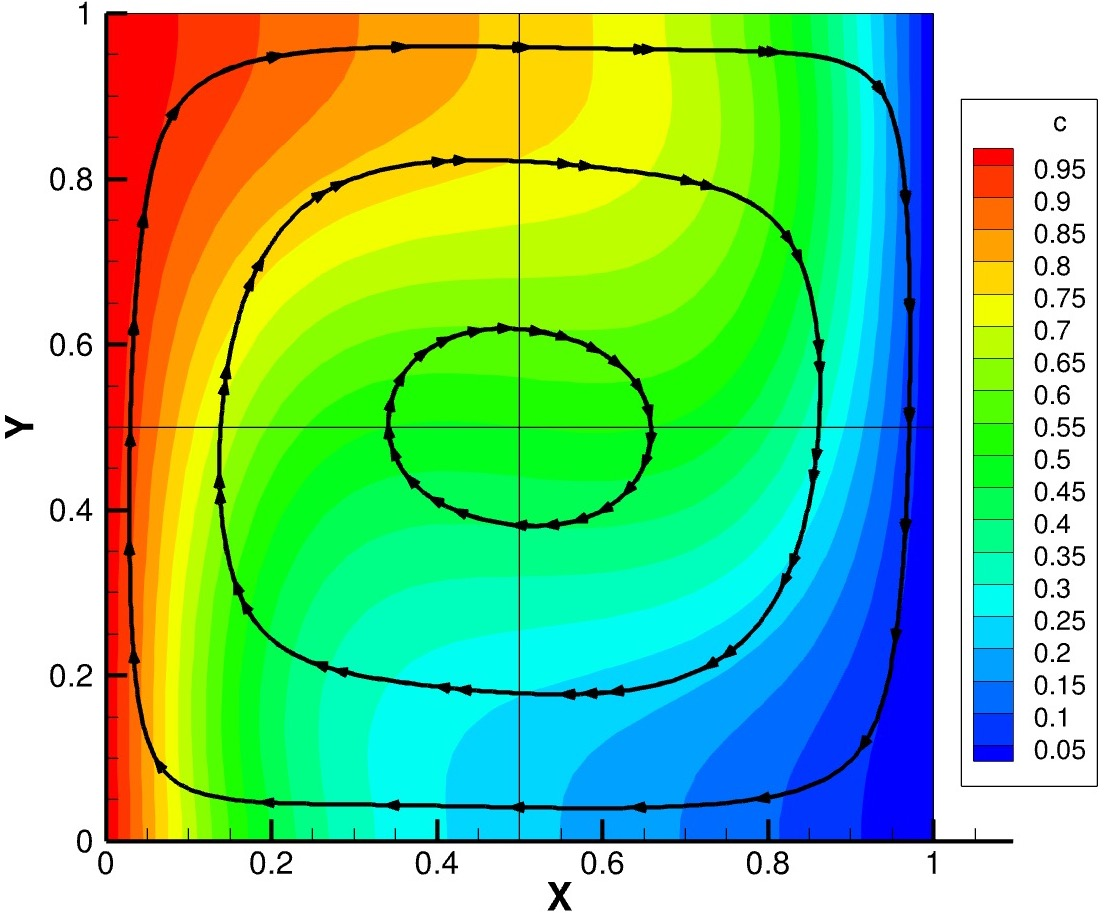
\includegraphics[width=0.6\textwidth]{tdrivcav}
\end{center}
\caption{
\label{fig.tdrivcav}
Solution for the buoyancy driven flow in a cavity: colour contours of
temperature overlaid with streamlines. Compare results for
$\Ra=1\times10^4$ in \citet{dvd83}. This image was produced using
\Tecplot.}
\end{figure}

%=============================================================================
\section{Boundary condition roundup}
\label{sec.bcs}

The basic types of boundary conditions the code can deal with are
Dirichlet type (value of variable is set, a.k.a.\ an \emph{essential}
boundary condition in the finite element community) and Neumann type
(boundary-normal gradient of value is approximated, a.k.a.\ a
\emph{natural} type boundary condition in the finite-element
community). The code can also deal with boundary conditions of mixed
type (a linear combination of Dirichlet and Neumann). We note that
periodic domain boundary surfaces (\verb|<P>|) are allowed, but
strictly speaking, periodicity does not constitute a boundary
condition as such.  Also we remark that for our code(s), boundary
conditions may only be set for variables involved in elliptic
sub-problems where, owing to the MWR treatment, Neumann boundary
conditions are implemented as integral approximations (which converge
to the given value pointwise as resolution is increased), while
Dirichlet conditions are `lifted' out of the problem and imposed
exactly to the values which are set by the user.

Standard Dirichlet and Neumann boundary conditions may be supplied as
a string that can be parsed by the solver to obtain a real value,
based on predefined and user-declared \verb|TOKENS|, and also the
space/time variables \verb|x|, \verb|y|, \verb|z| and \verb|t|.  These
strings are re-parsed at each time step, so time-varying boundary
conditions are allowed. We have already seen examples of these BC
declarations in \S\S\,\ref{sec.laplace}, \ref{sec.kovas}
and~\ref{sec.vb}.  Note that the strings involved should not contain
white space.  

We have not yet described mixed boundary conditions.  These are of
type $\partial c/\partial n+K(c-C)=0$ where $C$ and $K$ are constants.
Here, $n$ signifies the unit outward normal direction: $\partial
c/\partial n=\bm{n\cdot\nabla c}$.  Mixed boundary conditions are
specified in the form \verb|<M> field = mulval;refval </M>| where
\verb|mulval| is (a string that evaluates to) the real value $K$ and
\verb+refval+ is (a string that evaluates to) the real value $C$.  At
present for mixed BCs, unlike Dirichlet and Neumann boundary
conditions, $C$ and $K$ are fixed at the values they initially
evaluate to (not time-varying).

In \NavSto\ type problems, various of the above boundary conditions
for the velocity and pressure variables are typically combined in set
ways.  In some cases, the user does not provide values or choose the
combination since the boundary conditions are computed internally.
Below we supply as examples various typical boundary condition sets
which would be located in the \verb+BCS+ section of a session file.
As written, they are for \twoc\ \NavSto\ problems but the
generalisation to \threec\ problems should be obvious.

See also \S\,3.2 of the \Dog\ user guide for a discussion of sets of
boundary conditions appropriate for symmetry and anti-symmetry
boundaries.

%-----------------------------------------------------------------------------
\subsection{No-slip wall}

{\small
\begin{verbatim}
  <D> u = 0.0 </D>
  <D> v = 0.0 </D>
  <H> p       </H>
\end{verbatim}
}
\noindent The tag \verb+H+ for pressure (\verb+p+) denotes an
internally computed 'high-order' Neumann condition, as originally
described by \citet{kio91}.  If the associated \verb|GROUP| string is
\verb|wall| then tractions will contribute to the integrated values
found in \verb+session.flx+ file, see \S\,\ref{sec.flux}.

%-----------------------------------------------------------------------------
\subsection{Inflow or prescribed-velocity boundary}

{\small
\begin{verbatim}
  <D> u = 1.0 </D>
  <D> v = 0.0 </D>
  <H> p       </H>
\end{verbatim}
}
\noindent Note that either of the supplied values can be a string to
be evaluated by the parser at each timestep.

%-----------------------------------------------------------------------------
\subsection{Slip (no-penetration) boundary}

{\small
\begin{verbatim}
  <N> u = 0.0 </N>
  <D> v = 0.0 </D>
  <H> p       </H>
\end{verbatim}
}
\noindent Note that in this case, the boundary needs to be aligned
with the $x$ axis.  At present there is no way to set a slip boundary
which is inclined or curved; it must be parallel to either the $x$ or
$y$ axis.

%-----------------------------------------------------------------------------
\subsection{`Stress-free' outflow boundary}
\label{sec.stressfree}

{\small
\begin{verbatim}
  <N> u = 0.0 </N>
  <N> v = 0.0 </N>
  <D> p = 0.0 </D>
\end{verbatim}
}
\noindent This is a restricted approximation to a true stress-free
boundary where the tractions are zero. This boundary is also
stress-free but achieves the condition by ensuring that the viscous
and pressure tractions are individually zero, rather than their sum.

%-----------------------------------------------------------------------------
\subsection{Energy-stable open boundary}
\label{sec.robust}

{\small
\begin{verbatim}
  <O> u </O>
  <O> v </O>
  <O> p </O>
\end{verbatim}
}
\noindent This is a set of computed boundary conditions (computed
Robin/mixed for velocity and pressure).  These boundary conditions
were originally described in \citet{dong15} (see equations 37 and 38
there), and are based on maintaining boundedness of kinetic energy
within the domain.  It is an excellent combination for maintaining
stability for flows in short open domains, where the use of the
'stress-free' condition described in \S\,\ref{sec.stressfree} can lead
to catastrophe if significant inflow occurs over an outflow boundary,
or for allowing inflows on ingestion boundaries (such as outboard of a
jet issuing from a wall).  Type \verb|O| boundaries must set the string
\verb|open| in their associated \verb|GROUP|.  In addition one may set
the tokens \verb+DONG_UODELTA+ and \verb+DONG_DO+ \citep[see][these
  are $U_o\delta$ and $D_o$]{dong15}, with default values 0.05 and 1.0
respectively.  For a scalar variable ($c$), a zero Neumann condition
is set on these boundaries.

%-----------------------------------------------------------------------------
\subsection{Axis boundary}

{\small
\begin{verbatim}
  <A> u </A>
  <A> v </A>
  <A> p </A>
\end{verbatim}
}
\noindent
This is a set of Fourier-mode dependent homogeneous Dirichlet and
Neumann boundary conditions to be used when the boundary coincides
with the $x$ axis of a cylindrical coordinate system as described in
\citet{blsh04}. Type \verb|A| boundaries must set the string
\verb|axis| in their associated \verb|GROUP|.

%=============================================================================
\section{Fixing problems}
\label{sec.fix}

You are liable to come up against a few generic problems when making
and running your own cases. Here we will restrict discussion to
\NavSto\ problems and \verb+dns+.  The code will output an estimate of
the CFL-timestep every \verb+IO_CFL+ timesteps (default 50), along
with the average divergence of the solution (in the operator-splitting
used, incompressibility is only ensured in the spatial-convergence
limit).
%
The CFL estimate is generally quite reliable and provides guidance as
to which velocity component and element number is the most critical,
but also the divergence energy provides an excellent diagnostic of
trouble!
%
If velocity and length scales are of order unity, the reported
divergence energy should be much less than unity; if the divergence is
comparatively large then either the solution is blowing
up,\footnote{One wag suggested the name \Semtex\ was associated with
  this property of the solutions.} or the spatial resolution is
inadequate, or both.

By far the most common problem is that the solution will have a
CFL-type instability brought about by using too large a time-step;
this instability is unavoidably associated with using explicit time
integration for the advection terms in the \NavSto\ equations. This
problem is easily enough fixed: try reducing \verb+D_T+, and if
required, increasing \verb+N_STEP+ to maintain the same integration
interval. Obviously you will typically want \verb+D_T+ as large as
possible, so if the problem runs stably, increase the timestep as much
as is reasonable. If the velocity and timescales are of order unity,
then the maximum timestep would typically be of order two orders of
magnitude smaller (\verb+0.01+). Note that CFL-stability will decrease
with increasing time-integration order (\verb+N_TIME+).

If the solution persists in blowing up when the timestep is reduced,
the next most common cause is that there is inflow across an outflow
boundary (in which case the problem is ill-posed, however, in practice
\emph{some} inflow across an outflow boundary over restricted times
may be present without causing difficulty). To check if this is the
cause, you could put some history points near the outflow (see
\S\,\ref{sec.history}), but the best method of diagnosis is to run the
solution up to a time when divergence starts to increase markedly,
then use \Tecplot\ or some other postprocessor to examine the solution
near the outflow.  This problem has been largely circumvented in
\Semtex~V8 using the open BC set described by \citet{dong15}, see
\S\,\ref{sec.robust} above, though it cannot overcome all problems.
In pathological cases, fixing the problem will generally require the
mesh to be altered: sometimes the mesh is badly structured near the
outflow (\eg element sizes have been varied too rapidly); sometimes
the problem can be overcome by extending the domain downstream;
sometimes the domain needs to be reshaped (\eg by contracting it in
the cross-flow direction) so that there will be no outflow over the
inflow boundary. If all else fails, consider the methods of
\S\,\ref{sec.sponge} to force the velocity near the outflow to be
something more computationally tractable (if unphysical).

Finally: if you can't remember the syntax of a particular
\Semtex\ command, most of the executables will issue a usage prompt
when requested with the \verb|-h| command-line flag, along the lines
of regular Unix commands.  For example:
%
{\small
\begin{verbatim}
$ dns -h
Usage: dns [options] session-file
  [options]:
  -h       ... print this message
  -f       ... freeze velocity field (scalar advection/diffusion only)
  -i       ... use iterative solver for viscous steps
  -v[v...] ... increase verbosity level
  -chk     ... turn off checkpoint field dumps [default: selected]
  -S|C|N   ... regular skew-symm || convective || Stokes advection
\end{verbatim}
}
%
\noindent
If that is not enough help then you might consider examining at least
the header of associated source files, especially of the utilities.

%=============================================================================
\section{Execution speed}
\label{sec.speed}

%-----------------------------------------------------------------------------
\subsection{Serial (per processor) speed}

\Semtex\ makes good use of the BLAS, so it can be worth seeking fast
implementations. Especially, performance of the matrix--matrix
multiplication routine \verb+dgemm+ is critical. Many math libraries,
\eg \verb|openblas| and vendor-supplied math libraries such as AMD's
\verb|acml|, Intel's \verb|mkl| or Apple's \verb|Accelerate|
framework, now include some version of Kazushige Goto's fast
implementation of \verb|dgemm|.

As Reynolds numbers increase (\ie \verb+KINVIS+ decreases), the
viscous Helmholtz matrices in the operator splitting become more
diagonally dominant and better conditioned. In this case, you may find
that iterative (PCG) solution of the viscous step (obtained by setting
\verb|ITERATIVE=1| or running \verb|dns -i|) is actually faster than
the direct solution that is obtained by default. This is nice because
additionally, less memory is required. It is generally worth checking
this if you plan an extended series of runs, and Reynolds numbers are
large.

%-----------------------------------------------------------------------------
\subsection{Parallel execution}
\label{sec.mpi}

At present, the two primary solvers in \Semtex\ support parallel
MPI-based execution for \threed\ problems.  The associated solvers are
called \verb|elliptic_mp| (which gets little use\,---\,it mainly
exists for completeness and testing purposes) and \verb|dns_mp|.  If
an MPI system (\eg \verb|openmpi|, \verb|mpich|, \verb|lam/mpi|) is
present on your machine, the \verb|cmake| build system should detect
that and compile these two extra executables.

For \threed\ problems (\verb|N_Z|\,$\ge4$, see \S\,\ref{sec.nz}), the
solution can be made parallel across (\twod) Fourier modes.  No change
to the problem's \verb|session| file is required; one just needs to
change the executable from \verb|dns| to \verb|dns_mp| and pass
execution over to \verb|mpirun| (or local equivalent) for
administration.  The maximum number of processors which can be
employed is \verb|N_Z|\,$/2$, because each \twod\ Fourier mode is
complex (has real and imaginary parts), must be even, and must be
congruent with the 2-3-5 prime-factor FFT used.  (Don't be too
concerned: if you choose an inappropriate value, an error message will
be issued and execution will be terminated!).  Generally, parallel
speed-up will be initially somewhat linear with number of processors
used, but will eventually decay (see figure~\ref{fig:scaling}).

\begin{figure}
\begin{center}
  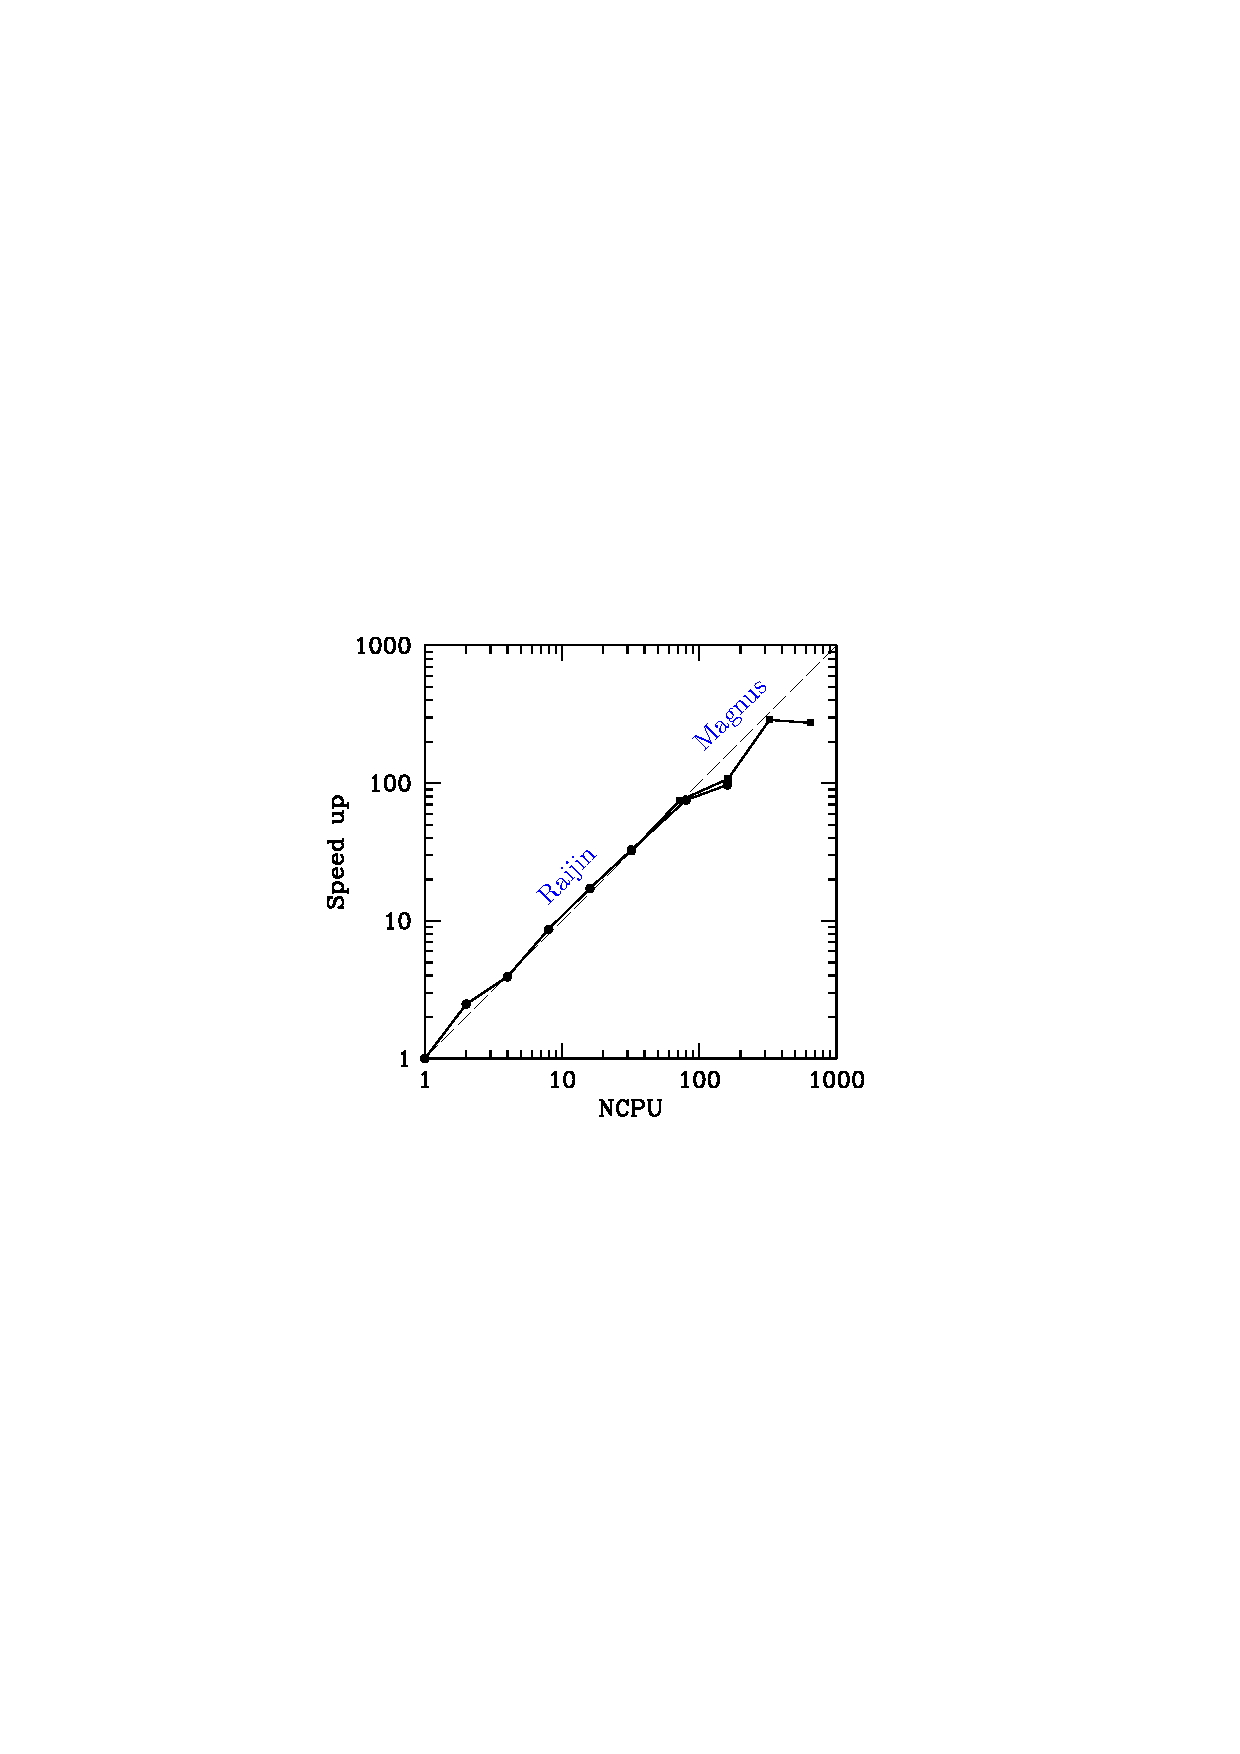
\includegraphics[width=0.5\textwidth]{HardScaling}
\end{center}
\caption{Hard scaling (speed-up for problem of a fixed size) relations
  for Fourier-parallel DNS of a turbulent pipe flow obtained at two
  different supercomputer facilities using MPI. The speed-up is
  approximately linear with number of processes until communications
  overheads become dominant (problem-dependent).  \citep[Reproduced
    from][]{blas19}.}
\label{fig:scaling}
\end{figure}

For example, the mesh used for the channel flow DNS examined in
chapter~\ref{ch.dns101} has \verb|N_Z|\,$=80$.  Then the maximum
number of processes which could be employed for parallel execution is
40.  However, the number of elements (96) is rather small, so one
could perhaps more efficiently use 20, or 10 (and maybe even as few as
8, 4 or 2) processors: one has to check the speed-up to see which is
most efficient, consider how long you are prepared to wait for results
and how many processors are available for use.

Here is how to use \verb|dns_mp| for that problem with 8 processors:
{\small
\begin{verbatim}
$ mpirun -np 8 dns_mp chan > /dev/null
\end{verbatim}}
\noindent
(Redirection of \verb|stdout| to \verb|/dev/null| is not necessary,
but once you are sure that the problem will run OK, is generally a
Good Idea.)

Apologies, but for now at least, none of the \Semtex\ utilities will
run in parallel.

%%%%%%%%%%%%%%%%%%%%%%%%%%%%%%%%%%%%%%%%%%%%%%%%%%%%%%%%%%%%%%%%%%%%%%%%%%%%%%
\chapter{Extra controls}
\label{ch.extra}

This chapter describes some additional features that are implemented
within the \NavSto\ solver \verb+dns+ to control execution and
output.

%=============================================================================
\section{Default values of flags and internal variables}
\label{sec.default}

There are two simple ways to establish the default values of all the
internal flags and variables used by \Semtex. The first is via
the \verb+calc+ utility: run \verb+calc -h+ and check the output (this
will also show you all the functions available to the parser for
calculating \verb+TOKEN+ variables, initial and boundary
conditions). The second is to examine the file
\verb+femlib/defaults.h+.

%=============================================================================
\section{Checkpointing}
\label{sec.check}

By default, intermediate solutions are written out as checkpoint dumps
in file \verb+session.chk+ every \verb+IO_FLD+ steps (default value
\verb+IO_FLD = 500+), rotating this to \verb+session.chk.bak+ so there
are usually two checkpoint files available for restarting if execution
stops prematurely (\eg if terminated by a queuing system or by a
floating point error).  Once the final time (\verb+N_STEP+) is
reached, the outcome (the terminal solution field) is written to
\verb+session.fld+.

Sometimes however, one wants a sequence of field dumps to be written
to \verb+session.fld+.  One can toggle this behaviour on the command
line using \verb+dns -chk+, or alternatively set the \verb+TOKEN+
\verb+CHKPOINT=0+ (the default being \verb+CHKPOINT=1+).  Beware:
turning off checkpointing can result in the generation of extremely
large \verb+session.fld+ files.

%=============================================================================
\section{Iterative solution}
\label{sec.iterative}

Two matrix solution methods are implemented for Helmholtz problems
associated with the viscous substep of the time splitting.  By
default, direct Schur-complement solutions are used.  The associated
global matrices can consume quite large amounts of memory, typically
much more than is required for storage of the associated field
variable.  Iterative (PCG) solution can also be selected, and this has
the advantage that since it is matrix-free, no global matrices are
required, however, solution may be slower than for the direct solver
(depending on the condition number of the global matrix problem).

The token that controls the selection of matrix solution method is
\verb+ITERATIVE+.  For \verb+dns+, PCG solution can be selected for
the viscous substep of the solution (\verb+ITERATIVE = 1+).  This can
also be selected via a command-line option (\verb+dns -i+), but note
that this overridden by tokens set in the \verb+session+ file (the
default value is \verb+ITERATIVE = 0+).

Iterative solution can be useful for the viscous substep, particularly
when the Reynolds number is high, since this decreases the condition
number of the associated global matrices.  In fact, iterative
solutions for the viscous substep can execute faster than direct
solutions at high Reynolds number, although this is platform
dependent. You should always consider trying \verb+ITERATIVE = 1+ as
an option for simulations where the Reynolds number is more than a few
hundred.


%=============================================================================
\section{Alternative forms of nonlinear terms}
\label{sec.nonlinear}

Various forms of the nonlinear terms for the \NavSto\ equations (\eg
$\bm{u\cdot\nabla u}$) are available.  The more standard ones are
generally selectable from the \verb+dns+ command line, but additional
forms can be selected via the token \verb+ADVECTION+ (which has
default value 1).  If you wish to solve the (unsteady) incompressible
Stokes equations for which the nonlinear terms are zero, set
\verb+ADVECTION = 5+ (or use \verb+dns -N+).  Owing to various vector
identities and incompressibility, $\bm{\nabla\cdot u}=0$, the various
nonlinear terms are equivalent in the continuum setting:
\[
\bm{u\cdot\nabla u} \equiv
\bm{\nabla\cdot uu} \equiv
\thalf[\bm{u\cdot\nabla u}+\bm{\nabla\cdot uu}] \equiv
\bm{u}\times\bm{\nabla}\times\bm{u} \equiv
\bm{u}\times\bm{\nabla}\times\bm{u} - \thalf\bm{\nabla u\cdot u}.
\]
The five forms above are generally named: convective (or, sometimes,
non-conservative), conservative, skew-symmetric, rotational-1 and
rotational-2.  While equivalent in the continuum setting, they have
somewhat distinct behaviours in the discrete (numerical) setting.

The convective form (standard in fluid mechanics texts) is generally
the simplest, and cheapest to compute (use \verb+ADVECTION = 2+ or
\verb+dns -C+).  Going back (at least) to the work of \citet{zan91b},
it is generally acknowledged that the skew-symmetric form has superior
energy conservation properties in the discrete setting and in our
experience is generally the most benign when solution resolution
starts to become marginal.  In early versions of \Semtex, this was the
default form (use \verb+ADVECTION = 0+ or \verb+dns -S+).  It does,
however, cost double to compute compared to the convective form.  A
simple variation, suggested by \citet{kerr85}, is to use the
convective and conservative forms on alternate timesteps --- this is
called the 'alternating' skew-symmetric form; `on average' one may
expect similar behaviour to the full skew-symmetric form, and it costs
much the same to compute as the convective form.  In our experience it
is about as robust as full skew-symmetric form, and since it is
cheaper, it has become the default option in \Semtex\ (use
\verb+ADVECTION = 1+ to explicitly select it).  It does, however, have
a slight defect: owing to alternation, it can produce small
high-frequency temporal oscillations in the solution, of period
$2\Delta t$.  It may also slightly reduce the asymptotic convergence
rates of steady solutions.  If you are seeking very clean solutions at
high resolution (\eg to compute base flows for stability analysis, or
your flow may have sensitive dynamics), it is best to use either
convective or full skew-symmetric forms.  In general, or perhaps when
computing, say, a turbulent flow, which is full of disturbance, you
might profitably use the default.

The two rotational forms are provided for completeness if you have a
specific interest in them --- use either \verb+ADVECTION = 3+ or
\verb+4+. Their computational cost is similar to the conservative
form. In summary:
\begin{tabbing}
xxxx\=ADVECTION = X \= xxxxxxxxxxxxxxxxxxxxxxxxxxx \= \kill
\> \verb+ADVECTION = 0+
\> $\thalf[\bm{u\cdot\nabla u}+\bm{\nabla\cdot uu}]$
\> \verb+dns -S+ \\
\> \verb+ADVECTION = 1+
\> $[\bm{u\cdot\nabla u}]^{(n)}~\textrm{or}~[\bm{\nabla\cdot uu}]^{(n+1)}$
\> (default) \\
\> \verb+ADVECTION = 2+
\> $\bm{u\cdot\nabla u}$
\> \verb+dns -C+\\
\> \verb+ADVECTION = 3+
\> $\bm{u}\times\bm{\nabla}\times\bm{u}$ \\
\> \verb+ADVECTION = 4+
\> $\bm{u}\times\bm{\nabla}\times\bm{u} - \thalf\bm{\nabla u\cdot u}$ \\
\> \verb+ADVECTION = 5+
\> $0$
\> \verb+dns -N+
\end{tabbing}

You may ask: what about the conservative form, $\bm{\nabla\cdot uu}$?
Isn't that as cheap to compute as the convective form?  Well, yes it
is, but \citet{wikl01} showed that it was also linearly unstable in a
discrete setting.  And, during development, our companion stability
analysis code, \verb+dog+, produced erroneous results when the
skew-symmetric form of advection terms was initially employed.  So,
the conservative form is not provided as an option for \verb+dns+ and
indeed, for this reason, the linearised advective term used by
\verb+dog+ ($\bm{u}'\bm{\cdot\nabla U}+\bm{U\cdot\nabla u}'$) is based
on the convective form.

Prior to \Semtex~V8, nonlinear product terms were dealiased in the
Fourier direction (only) when using the serial version of \verb+dns+.
Partly for consistency across serial and parallel computations, and
partly for simplicity, dealiasing was subsequently removed from the
code.  This can somewhat degrade the rate of exponential convergence
of results in the Fourier direction for serial execution, compared to
earlier releases.  Results for parallel execution are unchanged.

%=============================================================================
\section{Wall fluxes}
\label{sec.flux}

A file called \verb+session.flx+ is used to store the integral over
the \verb+wall+ group boundaries of viscous and pressure stresses (\ie
lift and drag forces).  Output is done every \verb+IO_HIS+ steps.  For
each direction ($x$, $y$, $z$), the outputs are in turn the pressure,
viscous, and total force per unit length (in $z$).  In 2D the
$z$-components are always zero, while in 3D the $z$-component pressure
force is always zero, owing to the fact that the geometry is invariant
in that direction.  For cylindrical geometries, the output values are
forces per radian (in the $x$ and $y$ directions) and torque per
radian (in the $z$ direction) rather than forces per unit length.

If a scalar (\verb+c+) is present in the simulation, then its integral
flux is also computed over the \verb+wall+ group boundaries and output
in the \verb+session.flx+ file, preceding the wall tractions.

%=============================================================================
\section{Wall tractions}
\label{sec.traction}

If the token \verb+IO_WSS+ is set to a non-zero value then the normal
and the single (2D) or two (3D) components of tangential boundary
traction are computed on the \verb+wall+ group, and output every
\verb+IO_WSS+ steps in the file \verb+session.wss+.  This is a binary
file with structure similar to a field dump.  The utility
\verb+wallmesh+ is used to extract the corresponding mesh points along
the walls (and can be used with \verb|sem2tec| to produce
\Tecplot\ input files). Note also that there is a stand-alone utility
called \verb+traction+ which is a post-processor that takes a standard
\verb|.fld| file and produces a wall traction file.

%=============================================================================
\section{Modal energies}
\label{sec.modal}

For \threed\ simulations (\verb+N_Z > 1+), a file of modal energies,
\verb+session.mdl+, is produced.  This provides valuable diagnostic
information for turbulent flow simulations.  For each active Fourier
mode $k$ in the simulation, the value output every \verb+IO_HIS+ steps
is 
\[
E_k =
\frac{1}{2A}\int_\Omega
\hat{\bm{u}}_k^\ast\cdot\hat{\bm{u}}_k \,{\rm d}\Omega,
\]
where $A$ is the area of the 2D domain~$\Omega$.  (In cylindrical
coordinate problems, the integrand is multiplied by radius.) Each line
of the file contains the time $t$, mode number $k$ and $E_k$.

Note that the \emph{energies are output only for non-negative Fourier
modes}.  To get the correct estimates for the one-sided spectrum (and
to satisfy Parseval's relation), the energies for non-zero modes
should be doubled.

%=============================================================================
\section{History points}
\label{sec.history}

History points are used to record solution variables at fixed spatial
locations as the simulation proceeds.  The locations need not
correspond to grid points, as data are interpolated onto the given
spatial locations using the elemental basis functions.  Locations of
history points are declared in the \verb+session+ file as follows:
%
{\small
\begin{verbatim}
<HISTORY NUMBER=1>
#       tag     x       y       z 
        1       0       0       0
</HISTORY>
\end{verbatim}
}
%
A file called \verb+session.his+ is produced as output.  Each line of
the file contains the step number, the time, the history point tag
number, followed by values for each of the solution variables.  The
step interval at which history point information is dumped to file is
controlled by the \verb+IO_HIS+ token; the default value is
\verb+IO_HIS = 10+.

%=============================================================================
\section{Averaging}
\label{sec.average}

Set \verb+AVERAGE = 1+ in the tokens section to get averages of field
variables left in files \verb+session.ave+ and \verb+session.avg+
(which are analogous to \verb+session.chk+ and \verb+session.fld+, but
\verb+session.ave.bak+ is not produced).  Averages are updated
every \verb+IO_HIS+ steps, and dumped every \verb+IO_FLD+ steps.
Restarts are made by reading \verb+session.avg+ if it exists.

Setting \verb+AVERAGE = 2+ will accumulate averages for Reynolds
stresses as well, with reserved names \verb+ABCDEF+, corresponding to
products
%
{\small
\begin{verbatim}
uu uv uw     A  B  D
   vv vw  =     C  E
      ww           F
\end{verbatim}
}
%
The hierarchy is named this way to allow accumulation of products in 2D
as well as 3D (for 2D you get only \verb+ABC+).  In order to actually
compute the Reynolds stresses from the accumulated products you need
to run the \verb+rstress+ utility, which subtracts the products of the
means from the means of the products:
\begin{verbatim}
rstress session.avg > reynolds-stress.fld
\end{verbatim}
An alternative function of \verb+rstress+ is to subtract one field
file from another:
\begin{verbatim}
rstress good.fld test.fld | convert | diff
\end{verbatim}

With the addition of scalar as well as velocity components, the
averaging (and naming) is extended in the following way:
%
{\small
\begin{verbatim}
uu uv uw  uc    A  B  D  G
   vv vw  uv =     C  E  H
      ww  uw          F  I
          cc             J,
\end{verbatim}
}
%
\noindent
again with a fairly obvious \twod\ restriction (\verb|ABCGHJ|).
Again, use \verb|rstress| to subtract products of means from means
of products.

Setting \verb+AVERAGE = 3+ will accumulate sums of additional products
for computation of terms in the kinetic energy transport equation. You
will then need to use the \verb+eneq+ utility to actually compute the
terms. Presently this part of the code is only written for Cartesian
coordinates, and only does collections based on kinetic energy.

%=============================================================================
\section{Phase averaging}
\label{sec.phase}

Phase averaging is useful for turbulent flows with a dominant (and
known) underlying temporal period.  We can collect statistics (with
\verb|AVERAGE=1|, \verb|2| or \verb|3|)\,---\,much as for the case
without phase averaging enabled\,---\,conditional on phase in the
cycle of the underlying period, see \citet{rehu72}.  Turning
on phase averaging does not preclude or stop collection of standard
statistics.  The enabling token is \verb|N_PHASE|, which must be a
positive integer; in addition one needs token \verb|STEPS_P| (steps
per period) which must be chosen such that \verb|STEPS_P| modulo
\verb|N_PHASE| is zero, and also \verb|N_STEP| modulo \verb|N_PHASE|
must be zero \emph{and} \verb|IO_FLD=STEPS_P/N_PHASE|.  Statistics are
written to files \verb|session.0.phs| \ldots \verb|session.X.phs|
where \verb|X=N_PHASE-1|.  The Reynolds stresses computed from these
files will represent fluctuations around the conditional average flow
at each phase point (the so-called `triple decomposition').

The slight difficulty is that if the period is not very well-defined
or we have a poor estimate of it, our sampling phase will slowly drift
unless we take corrective action.  However if the underlying period is
very well defined (\eg the flow is periodically forced) the method has
great potential.

%=============================================================================
\section{Particle tracking}
\label{sec.particle}

The code allows for tracking of massless particles, but this only
works correctly for non-concurrent execution at present.  Tracking is
quite an expensive operation, since Newton--Raphson iteration is used
to relocate particles within each element at every timestep.

The application looks for a file called \verb+session.par+.  Each line
of this file is of form
\begin{verbatim}
#     tag  time  ctime  x     y      z
      1    0.0   0.0    1.0   10.0   0.5.
\end{verbatim}
The \verb+time+ value is the integration time, while \verb+ctime+
records the time at which integration was initialised.

Output is of the same form, and is called \verb+session.trk+.  The use
of separate files, rather than by declaration in the session file, is
intended so that \verb+session.trk+ files can be moved to
\verb+session.par+ files for restarting.  Particles that aren't in the
domain at startup, or leave the domain during execution, are deleted.

Setting \verb+SPAWN = 1+, re-initiates extra particles at the original
positions every timestep.  With spawning, particle tracking can
quickly grow to become the most time-consuming part of execution.

%=============================================================================
\section{Spectral vanishing viscosity}
\label{sec.svv}

Spectral vanishing viscosity (SVV) amounts to implementing larger
viscosity at higher wavenumbers either in Fourier space or in spectral
element polynomial space.  The idea is that as resolution is increased
via $p$-refinement, the effect `vanishes' \citep{tadmor89,mot93}.  One
may regard SVV either as a type of implicit large-eddy simulation
methodology \citep{pasquetti06} or as a means of stabilising spectral
element solutions especially at high Reynolds numbers
\citep{xupa04,kish06}. Neither of these ideas has firm theoretical
underpinning at this stage, yet the method does appear quite effective
in reducing resolution requirements for turbulent flow simulations
\citep{ksb12,cnbmo15}.  Our implementation and nomenclature follows
the `standard method' described in \citet{ksb12}.  One can turn on SVV
separately and with different parameters for ($x$,\,$y$) spectral
elements and in the Fourier ($z$) direction.  These are all declared
in the \verb+TOKENS+ section.

\begin{tabbing}
XXXXXXX \= \kill
\texttt{SVV\_MN} \> Corresponds to cut-in mode $M_{zr}$ in 
spectral elements. Must be less than \texttt{N\_P}.\\ 
%
\texttt{SVV\_MZ} \> Corresponds to cut-in mode $M_\varphi$ in 
Fourier direction. Must be less than \texttt{N\_Z/2}.\\
%
\texttt{SVV\_EPSN} \> Corresponds to $\varepsilon_{zr}$. 
Should be a value larger than \texttt{KINVIS}, \eg \texttt{5*KINVIS}.\\
%
\texttt{SVV\_EPSZ} \> Corresponds to $\varepsilon_\varphi$. 
A value larger than \texttt{KINVIS}.
\end{tabbing}

The default polynomial transform in to place spectral element
expansions into a discrete hierarchical space is the discrete Legendre
transform \citep[see e.g.][]{blsc03}. This can be changed in
\verb|src/svv.cpp|.


%=============================================================================
\section{General body forcing}
\label{sec.dns_ff}

\textsl{This extension was largely developed by Thomas Albrecht.}\\

\noindent
If found, the \verb+FORCE+ section of the session file allows you to
declare various types of body forcing, \ie add a source term
to the RHS of the \NavSto\ equation. The currently implemented types
include (any combination allowed):\\[1em]
\begin{tabular}{rll}
 $ \bm{f} =$ & $\bm{f}_{const}$                           
  & constant force (frame acceleration)\\
           $+$ & $\bm{a_1}(\bm{x})$                       
  & steady, but spatially varying force\\
           $+$ & $\bm{a_2}(\bm{x}) \, \bm{\alpha}(t) $ 
  & modulated force\\
           $-$ & $m_1(\bm{x})\,(\bm{u} - \bm{u}_0)$  
  & sponge region\\
           $-$ & $m_2(\bm{x})\,(\bm{u}/|\bm{u}|)\,|\bm{u}(\bm{x}, t)|^2$  
  & `drag' force  \\
           $+$ & $\bm{\epsilon} G$                        
  & white noise    \\
           $-$ & $\chi(\bm{u}-\overline{\bm{u}})$
  & selective frequency damping \\
           $-$ & 2 $\bm{\Omega} \times \bm{u} - 
                    (\cd\bm{\Omega}/\cd t) \times \bm{x} -
                    \bm{\Omega} \times \bm{\Omega} \times \bm{x}$  
  & Coriolis force \\
           $-$ & $\beta_T(c-c_\textrm{ref})\bm{g}$
  & Boussinesq buoyancy.                
\end{tabular}\\[1em]

%----------------------------------------------------------------------------
\subsection{Constant force}
\label{sec.constant}

\noindent For example, a force constant in time and space $\bm{f} =
\bm{f}_{const}$ is declared by:
\begin{verbatim}
<FORCE>
        CONST_X = 4
        CONST_Y = 0
        CONST_Z = 0
</FORCE>
\end{verbatim}
This type of forcing must not be time or space dependent. It is suitable
for periodic channel flow, where you have a uniform and steady force
driving the flow, see \verb+channel-FX+ for an example session.

All forcing terms are applied in physical space.

Unless otherwise noted, any skipped keyword defaults to 0. Any line
starting with a hash \verb+#+ is ignored.

%----------------------------------------------------------------------------
\subsection{Steady force}
\label{sec.steady}

A spatially varying, steady force $\bm{f} = \bm{a}(\bm{x})$, computed
(or read from a file) during pre-processing and applied every time
step. See \verb|box-steady| for the complete example session. It suits
applications requiring localised, steady forcing.
\begin{verbatim}
<FORCE>
        STEADY_X =  cos(x)
        STEADY_Y = -sin(z)
        STEADY_Z = -cos(y)
        # STEADY_FILE = box-steady.force.fld
</FORCE>
\end{verbatim}

You may also point \verb+STEADY_FILE+ to a field file, in which case
the force is taken from the \verb+uvw+ fields of that file and
\verb+STEADY_[XZY]+ is ignored.
% The steady force may also be read from a field file by pointing
% \verb+STEADY_FILE = +$<$\textit{aFileName}$>$ to it. If so, the
% \verb+STEADY_[XZY] =+ lines are ignored, and the force is taken from
% \verb+lmn+ fields of the given file.\\[1em]
% \noindent\verb+compare box-steady > box-steady.force.fld+\\
% \verb+head box-steady.force.fld | grep Fields+\\
% \verb+uvwp+\fbox{\texttt{lmn}}\verb+                   Fields written+

%----------------------------------------------------------------------------
\subsection{Modulated force}

A spatially varying force, which is modulated in time, $\bm{f} =
\bm{a}(\bm{x}) \, \bm{\alpha(t)} $. The steady part $\bm{a}(\bm{x})$ is
computed (or read from a file) during pre-processing, while
$\bm{\alpha(t)}$ is evaluated each time step.
%See \verb|box-mod| for the complete example session.
\begin{verbatim}
<FORCE>
        # -- spatially varying part
        MOD_A_X =  cos(x)
        MOD_A_Y = -sin(z)
        MOD_A_Z = -cos(y)
        # MOD_A_FILE = box-mod.force.fld

        # -- time varying part
        MOD_ALPHA_X = step(t, 10)
        MOD_ALPHA_Y = step(t, 10)
        MOD_ALPHA_Z = step(t, 10)
</FORCE>
\end{verbatim}

%----------------------------------------------------------------------------
\subsection{Sponge region}
\label{sec.sponge}

This implements a so-called `sponge region' defined by the shape
function $m(x)$ in which a (physically meaningless) penalty term
$\bm{f} = m(\bm{x}) \, (\bm{u} - \bm{u}_0)$ forces the flow towards a
given solution $\bm{u}_0$.  It is especially useful for
inflow--outflow simulations of vortex shedding or turbulence: if the
velocity fluctuations hit the outflow boundary condition, they cause
unphysical reflections back into the domain which distort the upstream
flow. A sponge region placed just upstream the outflow boundary helps
to reduce the velocity fluctuations to (near) zero and thereby prevents
those reflections. The following section would apply the penalty term
for $20 \le x \le 24$, and within that region forces the velocity to
approach~$(1, 0, 0).$ That given solution may be a function of space,
but must be steady.
\begin{verbatim}
<FORCE>
        SPONGE_M = 5. * step(x,20)*heav(24-x)
        SPONGE_U = 1
        SPONGE_V = 0
        SPONGE_W = 0
</FORCE>
\end{verbatim}
%See \verb|cylinder17-sponge| for a more advanced example session.

%----------------------------------------------------------------------------
\subsection{'Drag' force}

An approximate drag force
$\bm{f} = - m(\bm{x}) \, (\bm{u}/|\bm{u}|)\, |\bm{u}(\bm{x},
t)|^2$.
Be aware that we use the previous time step's velocity $\bm{u}^{n}$ here.
\begin{verbatim}
<FORCE>
        DRAG_M = heav((x-2)^2 + y^2)
</FORCE>
\end{verbatim}
%See \verb+channel-FX-drag+ for an example session, where the drag
%force is applied in a circular region centered around (2, 0.5) in a
%laminar channel flow.

%----------------------------------------------------------------------------
\subsection{White noise force}

Similar to the \verb+noiz+ tool, this continuously adds random
perturbation $\bm{f} = (\epsilon_x, \epsilon_y, \epsilon_z)^T\,G$ in
specified direction, where $G$ is a normally distributed random
variable.  It is now only possible to apply the forcing uniformly in
physical space.
%Setting $\verb+WHITE_MODE+ \ge 0$ perturbs the given mode
%only, \ie \verb+WHITE_MODE = 2+ will perturb mode 2 only. Omitting
%this keyword or setting $\verb+WHITE_MODE+ < 0$ will apply white noise
%to all modes.

The following example applies white noise in $x-$direction to mode 0:
\begin{verbatim}
<FORCE>
        WHITE_EPS_X = 0.1
        WHITE_EPS_Y = 0
        WHITE_EPS_Z = 0
</FORCE>
\end{verbatim}
Adding white noise in all three directions degrades performance by
about 10\%. 
%See \verb+channel-FX-noiz+ for an example session.

%-----------------------------------------------------------------------------
\subsection{Selective frequency damping (SFD)}
\label{sec.sfd}

This is a means of obtaining an approximate steady state solution to
the \NavSto\ equations using an unsteady solver, originally described
by \citet{abhhms06}. SFD applies a penalty term of the form
$-\chi(\bm{u}-\overline{\bm{u}})$ to the right-hand side of the
momentum equations, where $\overline{\bm{u}}$ is an estimate of the
time-mean solution that is updated as integration proceeds (and held
in internal storage). SFD can also be considered as applying an IIR
low-pass digital filter to the discrete approximation of the
\NavSto\ equations.

The two parameters are \verb|SFD_CHI| (\ie penalisation multiplier
$\chi$) and \verb|SFD_DELTA|, which is the time constant $\Delta$ used
in updating a forwards-Euler approximation of the steady flow
$\overline{\bm{u}}$ (see reference).  Both values are problem-specific
and should be tuned to get acceptable results.  Note that it is not
always possible to obtain a steady outcome with SFD, and that it is
generally preferable to use standard skew-symmetric form of the
nonlinear terms for \verb|dns|, rather than the now-default
alternating skew symmetric form: this can be achieved by setting token
\verb|ADVECTION = 0| or by using command-line flag \verb|-S| with
\verb|dns|.

\begin{verbatim}
<FORCE>
        SFD_CHI   = 0.2
        SFD_DELTA = 0.75
</FORCE>
\end{verbatim}

A final point to note is that the values of the two parameters are
parsed once, at the beginning of runtime, after any restart file (if
present) is read.  Thus, their definitions can contain the temporal
variable \verb|t|, but the value used is whatever holds at the start
of runtime.

%----------------------------------------------------------------------------
\subsection{Rotating frame of reference: Coriolis and centrifugal force}
\label{sec.rotating}

% @book{batchelor2000,
%   title={An introduction to fluid dynamics},
%   author={Batchelor, G.K.},
%   year={1967},
%   publisher={Cambridge University Press}
% }

If the flow is to be computed in a rotating frame of reference,
additional acceleration terms appear, namely $\bm{f} = -2\,\bm{\Omega}
\times \bm{u} - (\cd\bm{\Omega}/\cd t) \times \bm{x} -\bm{\Omega}
\times (\bm{\Omega} \times \bm{x})$ \citep{bat67}. The vector
of rotation $\bm{\Omega}$ is \emph{always} given in Cartesian
co-ordinates, even if \verb|CYLINDRICAL = 1|. Its magnitude and/or
orientation can change with time. However, the axis of rotation it is
always assumed to go through the origin. Depending on whether
$\bm{\Omega}$ is steady or not, usage slightly differs.


For unsteady $\bm{\Omega}$, set the flag \verb|CORIOLIS_UNSTEADY = 1|
and give $\bm{\Omega}$ and $\cd\bm{\Omega}/\cd t$. All terms are
re-evaluated each time step.
\begin{verbatim}
<TOKENS>
        f        = 1.
        omega    = TWOPI * f
</TOKENS>

<FORCE>
        CORIOLIS_UNSTEADY = 1

        CORIOLIS_OMEGA_X = 0
        CORIOLIS_OMEGA_Y = 0
        CORIOLIS_OMEGA_Z = omega * sin(t)

        CORIOLIS_DOMEGA_X_DT = 0
        CORIOLIS_DOMEGA_Y_DT = 0
        CORIOLIS_DOMEGA_Z_DT = omega * cos(t)
</FORCE>
\end{verbatim}

\noindent 
For constant $\bm{\Omega}\neq f(t)$, the term
$-(\cd\bm{\Omega}/\cd t)\times\bm{x}$ vanishes, and the centrifugal
force $-\bm{\Omega} \times (\bm{\Omega} \times \bm{x})$ can be
computed during pre-processing.
%
Set \verb|CORIOLIS_UNSTEADY = 0| and make sure to include the centrifugal
force manually using a steady force as it is no longer computed automatically%
\footnote{If you're lazy, or for cross-checking, you could set
  \texttt{CORIOLIS\_UNSTEADY = 1} and omit
  \texttt{CORIOLIS\_DOMEGA\_[XYZ]\_DT} to have the centrifugal term
  computed automatically. Note, however, that this degrades
  performance as it is done each time step.}.  A temporal derivative
$\cd\bm{\Omega}/\cd t$, if given, is ignored.

\begin{verbatim}
<FORCE>
        CORIOLIS_UNSTEADY = 0

        CORIOLIS_OMEGA_X = 0
        CORIOLIS_OMEGA_Y = 0
        CORIOLIS_OMEGA_Z = omega

        # -- centrifugal term for Omega = (0, 0, omega)^T
        #    for a cylindrical problem
        STEADY_X = x*omega^2
        STEADY_Y = omega^2*y*(cos(z)^2)
        STEADY_Z = -omega^2*y*cos(z)*sin(z)
</FORCE>
\end{verbatim}

% A sample session \verb+box-coriolis+ makes use of steady forcing to let
% the flow approach a given (divergence-free) solution, taking into
% account this coriolis term.
%\noindent See \verb|cylkovrot| for an example session.

See \citet{ablmm15} for an example of DNS carried out in a rotating
frame of reference.

%----------------------------------------------------------------------------
\subsection{Boussinesq buoyancy}
\label{sec.bous}

See the example of \S\,\ref{sec.tdrivcav}. This option is available if
your simulation includes a scalar, in which case it can be considered
as a temperature, allowing for the introduction of body forces based
on density variation produced by a coefficient of thermal expansion
$\beta_T$.  In the Boussinesq approximation, the flow is still assumed
to be incompressible, and the added body force is of form
$-\beta_T(c-c_\textrm{ref})\bm{g}$, where $c_\textrm{ref}$ is a
reference value of scalar (\ie temperature) and $\bm{g}$ is the
gravitational acceleration vector.  Note that for an ideal gas,
$\beta_T=1/c_\textrm{ref}$.

\begin{verbatim}
<FORCE>
        BOUSSINESQ_TREF    = 288.15
        BOUSSINESQ_BETAT   = 1./BOUSSINESQ_TREF
        BOUSSINESQ_GRAVITY = 10.
        BOUSSINESQ_GY      = -1.0
</FORCE>
\end{verbatim}

The gravity vector is supplied as a magnitude,
\verb|BOUSSINESQ_GRAVITY|, and a set of direction cosines; in the
above example, only the $y$ component is set, with the other
components defaulting to zero.  If cylindrical coordinates are
employed, only the axial, $x$, direction cosine is used, \ie the
gravity vector must be aligned with the axis of the coordinate system.
For historical reasons, the scalar $c$ goes under the pseudonym
\verb|T| here, \ie $c_\textrm{ref}\equiv\verb|BOUSSINESQ_TREF|$

A further restriction to note is that while, logically, buoyancy
forces should recognise potential-type reference frame forces (such as
rotation), at present this is not implemented, so that buoyancy only
responds to gravity fields.

As of 2022, this kind of gradient-based Boussinesq treatment has been
deprecated in favour of the more complete approach described in the
following section.

%----------------------------------------------------------------------------
\subsection{`Canonical' steady Boussinesq buoyancy}
\label{sec.csb}

This is the treatment of Boussinesq buoyancy described in
\citet{blss21}, whereby density fluctuation is applied to all the
convective and frame-acceleration terms in the \NavSto\ equations.  In
fact, here, it is applied to the convective, frame-acceleration,  and
any other forcing terms.  (It is usual in GFD Boussinesq applications
to apply density variation only to gravitational body
force\,---\,equivalent to a frame acceleration\,---\,on the assumption
that this is typically large compared to the fluid acceleration
terms.)

Following from \citet{blss21}, the canonical Boussinesq treatment of
the incompressible \NavSto\ equations (\S\,\ref{sec.pdes}) is
(with body force terms $\bm{f}$ included, and transposed onto the LHS
of the momentum equation)
\begin{equation}
  \frac{\rho}{\rho_0}\left[\frac{\cD\bm{u}}{\cD t}-\bm{f}\right] = \left(1 +
  \frac{\rho'}{\rho_0}\right)\left[\frac{\cD\bm{u}}{\cD t}-\bm{f}\right]=
  -\frac{1}{\rho_0}\bm{\nabla}p+\nu\nabla^2\bm{u}, \quad \bm{\nabla\cdot u}=0,
\label{eq.full}
\end{equation}
where $\bm{u}$ is the velocity field measured in an inertial frame of
reference.  Using the typical approach where the effect of density
variation is dropped from the local accelerative term, the momentum
equation above is approximated as
\begin{equation}
  \frac{\partial\bm{u}}{\partial t} +
  \left(1+\frac{\rho'}{\rho_0}\right)\left[\bm{u\cdot\nabla u} +
   2\bm{\Omega}\!\times\!\bm{u} + \bm{\Omega}\!\times\!(\bm{\Omega}\!\times\!\bm{r}) +
  \bm{\alpha}\!\times\!\bm{r} + \bm{A} -\bm{f}\right]
  =   -\frac{1}{\rho_0}\bm{\nabla}p+\nu\nabla^2\bm{u},
\label{eq.denacc1}  
\end{equation}
where now $\bm{u}$ is measured relative to the origin of the
arbitrarily accelerating and rotating frame of reference.  As in our
standard treatment of Boussinesq buoyancy (\S\,\ref{sec.bous}) the
relative density variation
$\rho'/\rho_0=\beta_T(T_\text{ref}-T)\equiv\beta_T(c_\text{ref}-c)$.
Equation \eqref{eq.denacc1} is the `canonical steady Boussinesq'
treatment of buoyancy terms.  As explained in \citeauthor{blss21}, it
is a robust treatment of Boussinesq buoyancy and fulfils the original
intention in the case of steady flows\,---\,and the omission of effect
of density variation on the local acceleration term is also a part of
standard Boussinesq treatments, so in effect it is a more complete
approach than the standard method.  Note that the flows considered
need not be steady; it is just the case that, as for standard
Boussinesq treatments, the approximation is more complete when they
are.  We call the method the convective--frame-acceleration Boussinesq
treatment (that's a mouthful, so we use the acronym CFB below).

As outlined in \citeauthor{blss21}, a gravitational field $\bm{g}$
would be included as a frame acceleration term $\bm{A}\equiv-\bm{g}$
and dealt with using the approach described in \S\,\ref{sec.constant}.
Any frame-rotation terms would be dealt with as described in
\S\,\ref{sec.rotating}.

\begin{figure}
  \begin{center}
    \begin{tabular}{cccc}
      \raisebox{26ex}{(\textit{a})} & 
      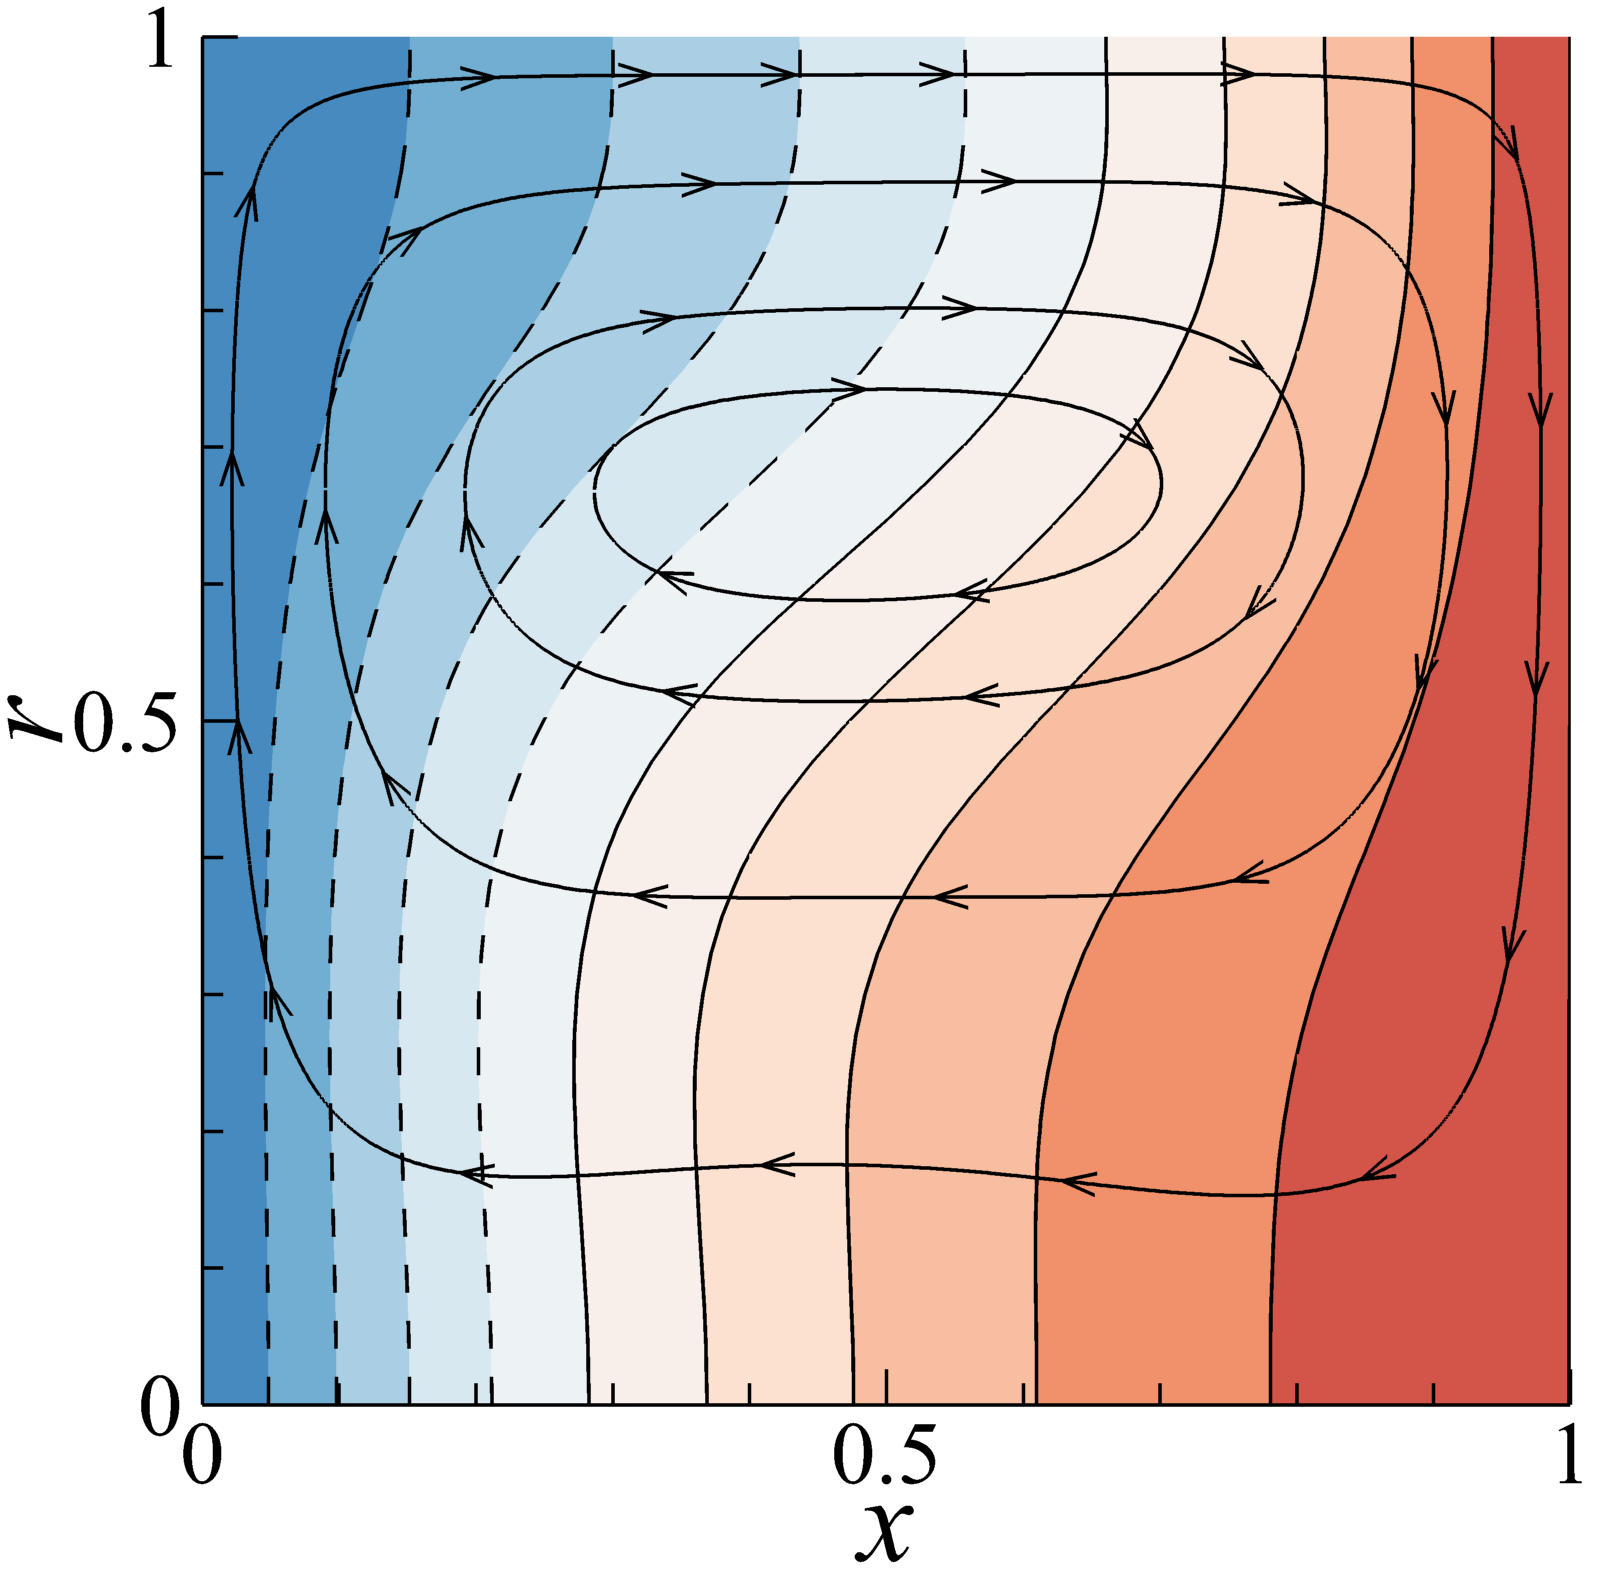
\includegraphics[height=0.2\textheight]{MMBL} &
      \raisebox{26ex}{(\textit{b})}&
    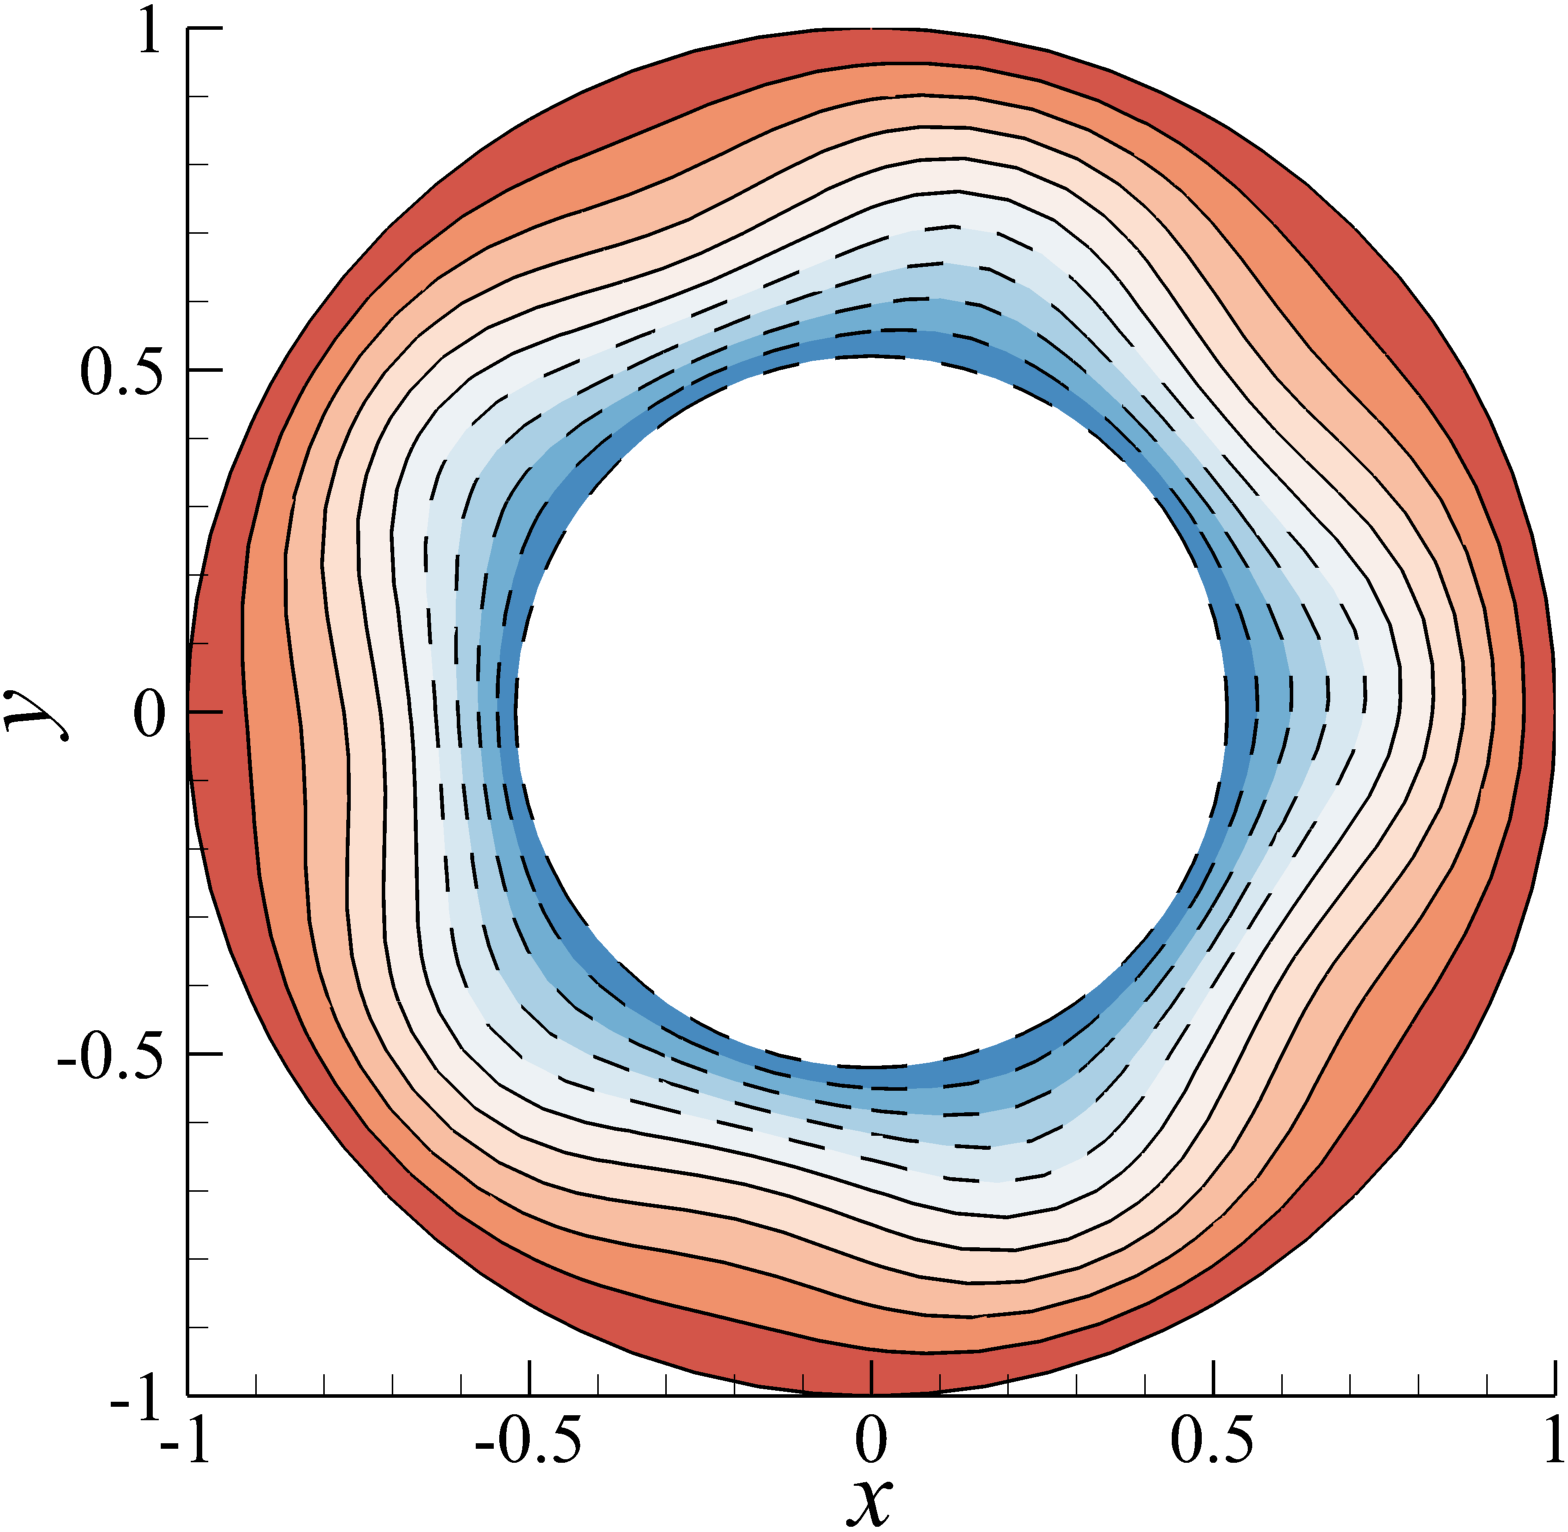
\includegraphics[height=0.21\textheight]{PCM2}
    \end{tabular}
  \end{center}
  \caption{ Canonical steady buoyancy test case examples from
    \citet{blss21}.  Red/blue colours indicate warm/cool fluid.  See
    supplied session files \texttt{MMBL} and \texttt{PMC2}. }
  \label{fig.csb}
\end{figure}

To use CFB buoyancy, one needs to define \verb|CFB_BETA_T| and
\verb|CFB_T_REF| in the \verb|FORCE| section.  These are equivalent to
the regular Boussinesq tokens outlined in the previous section. In
addition, one may need to apply frame acceleration terms as outlined
above in \S\S\,\ref{sec.constant}, \ref{sec.steady}
and~\ref{sec.rotating}.

For example, consider the case dealt with in \citet{blss21} \S\,3.1,
see the present figure~\ref{fig.csb}(\textit{a}).  This is an
axisymmetric rotating flow dealt with in cylindrical coordinates.  It
has frame acceleration in the $-x$ direction, which is equivalent to a
steady body force in the $+x$ direction.  As explained in
\S\,\ref{sec.rotating}, we can set \verb|CORIOLIS_UNSTEADY=0| and
explicitly add a steady (centrifugal) body force $|\bm{\Omega}|^2r$
--- this is computationally cheaper than computing
$-\bm{\Omega}\times(\bm{\Omega}\times\bm{x})$ at every timestep.  We
still need to set \verb|CORIOLIS_OMEGA_X| to ensure the Coriolis body
force terms $-2\bm{\Omega}\times\bm{u}$ are computed.  Here is the
\verb|FORCE| section for that example (see also session file
\verb|MMBL| in the \verb|mesh| directory).  The supplied values in
various of the assignments below correspond to user-defined
\verb|TOKENS|.

\begin{verbatim}
<FORCE>
    CFB_BETA_T        = BETA_T
    CFB_T_REF         = T_REF
    CORIOLIS_UNSTEADY = 0
    CORIOLIS_OMEGA_X  = OMEGA
    STEADY_Y          = OMEGA*OMEGA*y
    CONST_X           = GRAVITY
</FORCE>
\end{verbatim}

Another example is the test case of \citet{blss21} \S\,3.2, see
present figure~\ref{fig.csb}(\textit{b}).  This is a rotating flow,
and the geometry and boundary conditions are again axisymmetric, but
the problem is dealt with in Cartesian coordinates (which allows the
$k=5$ wavy primary instability to develop in 2D). There is no
gravitational acceleration in this case.  Note the treatment of the
centrifugal force terms.  See also the session file \verb|PCM2| in the
\verb|mesh| directory.

\begin{verbatim}
<FORCE>
    CFB_T_REF         = T_REF
    CFB_BETA_T        = BETA_T
    CORIOLIS_UNSTEADY = 0
    CORIOLIS_OMEGA_Z  = OMEGA
    STEADY_X          = OMEGA*OMEGA*x
    STEADY_Y          = OMEGA*OMEGA*y
</FORCE>
\end{verbatim}

By default, hydrostatic pressure gradients associated with steady body
forces or accelerations are removed for CFB.  This is convenient in
the case that there are free boundaries and one does not wish to apply
associated pressures.  If you wish hydrostatic terms to appear, you
should also set \verb|CFB_REMOVE_HYDRO=1|.
 

%%%%%%%%%%%%%%%%%%%%%%%%%%%%%%%%%%%%%%%%%%%%%%%%%%%%%%%%%%%%%%%%%%%%%%%%%%%%%%
\chapter{Code design and the \Semtex\ API}
\label{ch.api}

%\textsl{This chapter is in development.}\\


While the top level of the code is written in \cpp, the bulk of
computational work is carried out using 3rd-party libraries: BLAS and
LAPACK (vendor- or distribution-supplied) for \twod\ operations,
Temperton's 2-3-5 prime factor FFT (incorporated into \texttt{femlib})
for \threed\ operations, and (open)MPI for parallel operations.
Depending on what your application hits the hardest, one or other of
these things may be the speed-determining component. Optimising
compilers are liable to make a only a small difference\,---\,most
speed-up is now to be achieved by further algorithm development.
However, it is definitely worthwhile seeking out a fast BLAS library
(as supplied with Apple's Xcode, Intel's MKL, or AMD's ACML).

Some fundamental design decisions:
\begin{enumerate}
\item
  In \Semtex, all floating point numbers are double precision
  variables.
\item
  Most real-type data arrays are flat (\oned).  In C and \cpp, such
  arrays have indices starting at 0, while in Fortran, indexing starts
  at 1 by default\,---\,though the start address is identical. This
  makes them easy to use with Fortran routines, but with the following
  caveat.
\item
  The layout of these flat arrays are typically taken as row-major,
  which is standard C/\cpp. However, Fortran uses column-major
  ordering. For this reason, any BLAS or LAPACK matrix operation may
  at first sight seem to be the transpose of what is intended.
\item
  Ordering of storage in data \verb|AuxFields| is, working bottom-up:
  $(x,y)$ data in each element with internal row-major order starting
  from the bottom-left corner (\ie at the first vertex), then a list
  of elements as declared in the \verb|ELEMENTS| section of the
  session file, then by $z-$planes.
\item
  Most low-level \cpp\ methods in the code do not incorporate internal
  data storage but can be regarded as operator routines, and get
  handed addresses to appropriate parts of storage from within the
  flat data arrays on which to work.
\end{enumerate}

Coding conventions:
\begin{enumerate}
\item
Class private or protected member data names start with an underscore,
\eg \texttt{\_ntot}.
\end{enumerate}

%=============================================================================
\section{Useful things to know about}

\begin{description}

\item[Hierarchy of main data storage] From top down: \verb|Domain|,
  \verb|Field|s, \verb|AuxField|s, \verb|Element|s. The key entity for
  most applications programming is the \verb|AuxField| class, which
  contains scalar field variables and a list of \verb|Element|
  pointers.  The \verb|Field| class inherits from the \verb|AuxField|
  class, adding a list of boundary condition applicators and the
  ability to solve elliptic problems.  The \verb|Domain| class holds
  an array of \verb|Field| pointers and most of its internal storage
  is publicly accessible.
  
\item[The Geometry class] This class (\verb|src/geometry.cpp|)
  centralises information about the `logical' (rather than `spatial')
  geometry of the solution domain, for example, the number of points
  along the edge of each element, the number of elements, number of
  processes, the total number of $z$-planes, the number of $z$-planes
  per process, the number of Fourier modes, the number of data in a
  single $(x,y)$ plane, etc.

  Most of these are fairly straightforward (peruse \verb|geometry.h|),
  but it may be worthwhile to explain the distinction between
  \verb|Geometry::nPlane()| and \verb|Geometry::planeSize()|.  The
  first of these is simple to understand: the number of elements
  multiplied by the number of points in each element.  The second is
  similar, but often somewhat larger, because of (a) restrictions
  brought on by the FFT used (the number of points in a plane must be
  even if the solution is \threed\ and an FFT will be used in the
  orthogonal direction) and (b) further requirements for parallel
  execution, which requires block-transposes of data across
  processes, as explained in \citet{rb06}.  In each case, the extra
  padding does not end up entering computations.  The amount of data
  allocated internally for each data plane is
  \verb|Geometry::planeSize()|.  A consequence of this distinction is
  that the memory for the first storage location in any data plane
  does not necessarily immediately follow that for the last storage
  location of the preceding plane.  In an \verb|AuxField|, the
  variable \verb|_plane| references a set of pointers to the first
  storage location of each plane on the current process.

%\item[Nodal elements] the shape functions used in the code correspond
%  to the classical `nodal', rather than the `modal' scheme. This means
%  that the shape functions are tensor products of 1D Lagrange
%  interpolants that have value unity at one mesh node and zero at the
%  others.
  
\item[Timestepping algorithm, storage schemes] The time integration
  scheme used in \verb|dns| is the `stiffly stable' algorithm, based
  on backward differencing in time, and uses time-splitting as
  originally described in \citet{kio91}. What is stored where, and
  when\,---\,see figure~\ref{fig.storage}.
  
%\item[Boundary conditions and inheritance] Distinction between the way
%  BCs are dealt with. Note: periodicity technically does not
%  constitute a boundary condition.
  
\item[Support libraries and static member functions] The two
  base-class libraries provided as part of \Semtex\ are called
  \verb|veclib| and \verb|femlib|. \verb|Veclib| provides vector
  algebra primitives and can be regarded as an extension to the BLAS:
  check \verb|veclib/README| for a summary of the operations it
  provides.  \verb|Femlib| is a bundle of low-level operations that
  are finite-element and spectral-element-shape function related, 
  also provides the parser (\verb|femlib/initial.y|) and
  message-passing routines, as well as Fourier transforms.

  It is standard to use library-name prefixes on calls to these
  libraries, as well as for LAPACK and BLAS calls (\verb|Veclib::|,
  \verb|Femlib::|, \verb|Lapack::|, \verb|Blas::|) to help the
  programmer identify the libraries involved.
%  (These things could all
%  be \verb|namespace|d, but are not, partly because the header files
%  used to recruit all the calls into static member functions preceded
%  the introduction of namespaces into \cpp.)
  
\item[BLAS-conformant increments] Where access to a block of data is
  obtained on the offset, skip model, this is done in a
  BLAS-conformant way if the skip is negative: the start address is at
  the high end of the memory space.

\item[Implications of Fourier transform in one direction] For
  \threed\ computations, note that for all of the timestepping loop,
  other than during computation of the nonlinear terms, field
  variables are held in the Fourier-transformed state.  Field data
  written out to file are in physical space.
  
\item[Static condensation] Because finite/spectral element shape
  functions can be partitioned into sets which do/do not have non-zero
  support at the edges of elements, and because global Galerkin shape
  functions have only comparatively local support (confined to mating
  finite elements), only element-edge variables need to be considered
  when assembling the global Galerkin forms of elliptic equations.
  Subsequently, remaining element-internal variables can be obtained by
  local solutions on an element-by-element basis.  Recognition of this
  fact has long been a part of finite-element procedures, where it
  goes under various names: substructuring; static condensation;
  Schur-complement solution.  \Semtex\ uses this methodology for
  assembly and solution of elliptic equations when direct methods are
  used.

%\item[Tensor-product derivative operations]

%\item[Direct versus iterative solves]
  
\item[Message passing and data exchange] One key simplification
  regarding message passing: \emph{all} MPI calls used by \Semtex\ are
  contained within \verb|femlib/message.c|, and the number of MPI
  routines used is comparatively small.

\item[Contents of main directories] The following directories are
  present in the distribution: \verb|include| which has copies of
  header files; \verb|src| which holds \cpp\ source code for the
  classes shared by \Semtex\ applications; \verb|veclib| which holds
  routines for many standard loops over vectors, with a mnemonic
  naming convention (the code here is almost exclusively written in
  C); \verb|femlib| has \oned\ spectral polynomial routines (knot and
  quadrature point computations, differentiation matrix construction)
  and FFTs, all written in either C or Fortran77; \verb|utility|
  routines for pre and post-processing; \verb|test| which has code
  validity regression tests, with the `right answers' stored in
  \verb|regress|; \verb|mesh| holds a selection of session files.  The
  two main application code directories are \verb|elliptic| and
  \verb|dns| which have been described in earlier chapters.  The
  \verb|sm| directory contains useful \SM\ macros, while the
  \verb|python| directory has some useful scripts for data processing.
  
\end{description}

The code has a fair amount of low-level optimisation built in for
vector computer architectures, but it's not compiled in by default. To
get vector-optimised routines, add \verb+-D_VECTOR_ARCH+ to the
section of \texttt{src/Makefile} appropriate to your machine. Also you
may want to try altering the parameter \texttt{LVR} in
\texttt{src/temfftd.F} if your job makes heavy use of FFTs.

\begin{figure}
\begin{center}
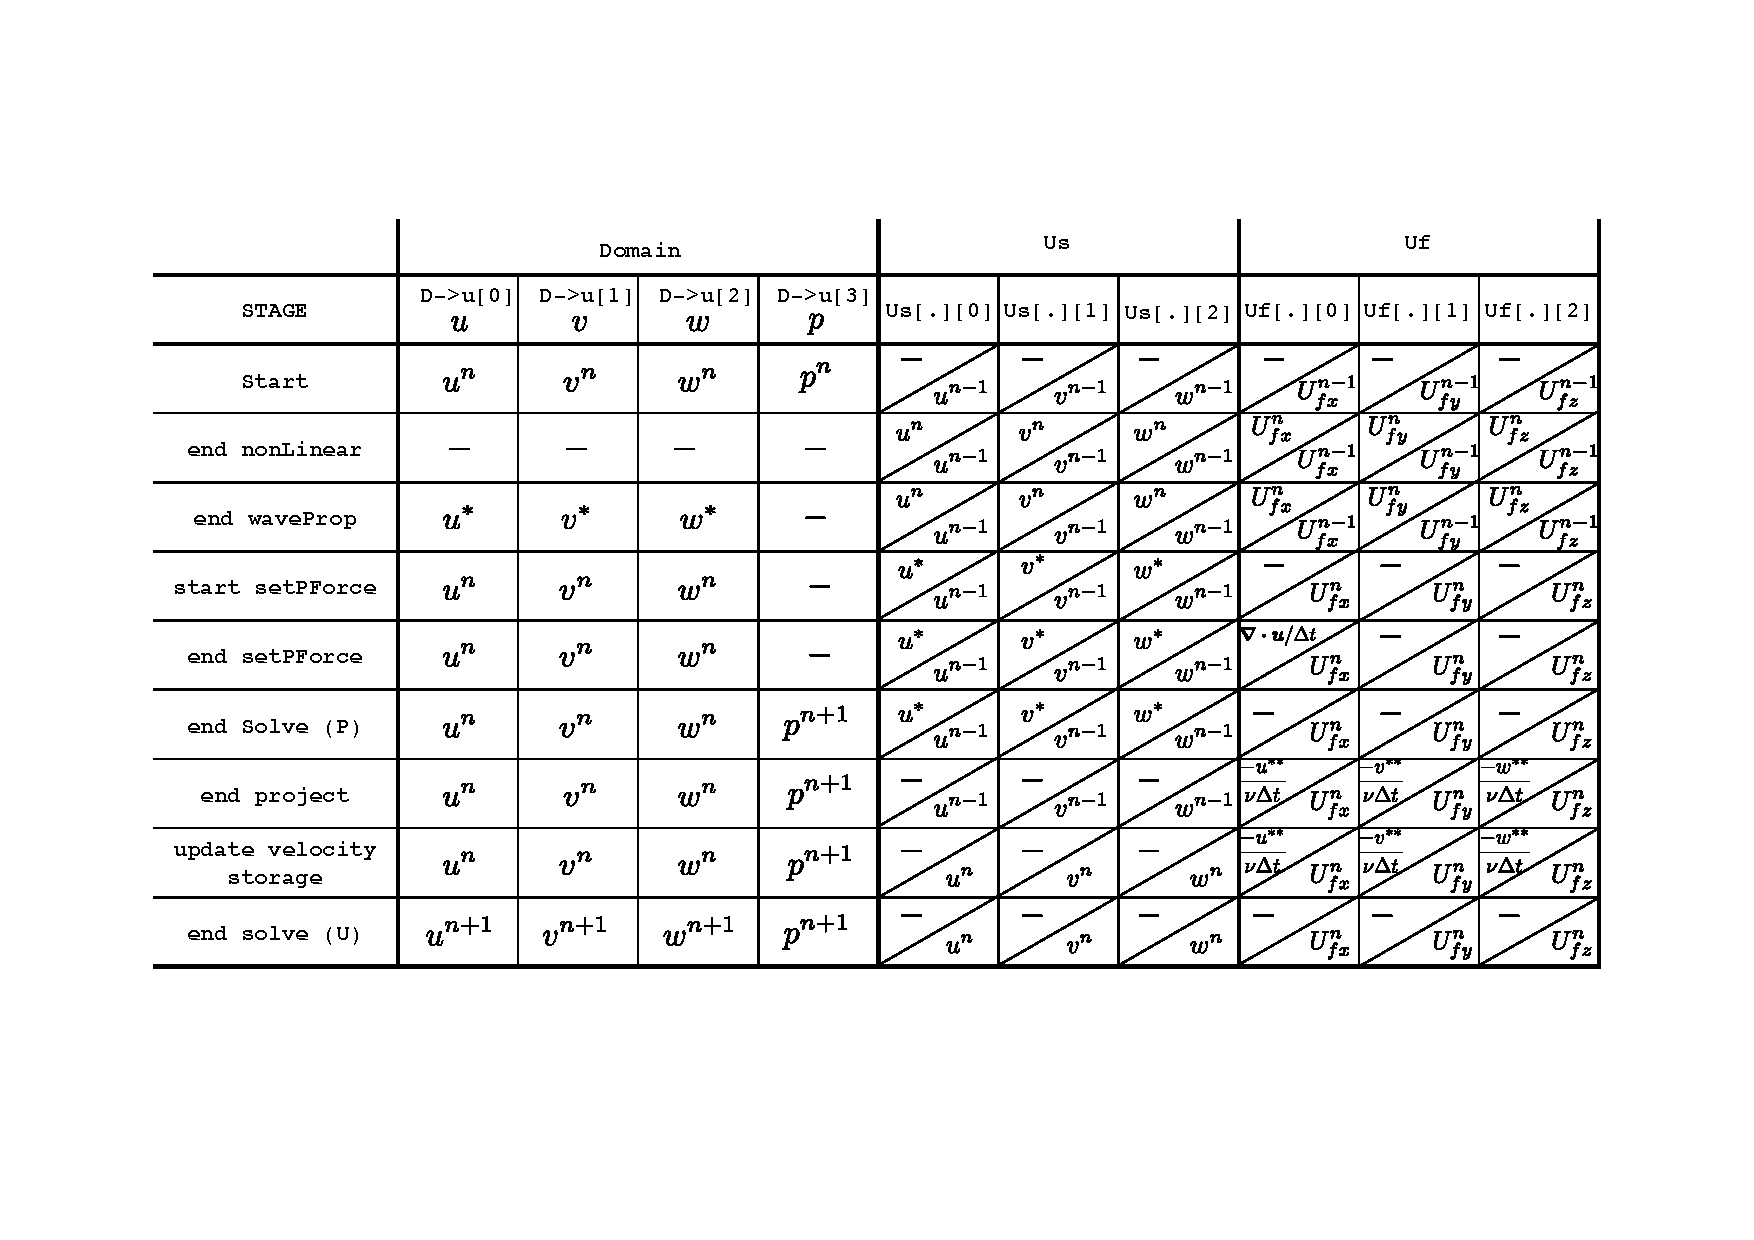
\includegraphics[width=\textwidth]
{timeSchemeStorage}
\end{center}
\caption{Arrangement of internal storage during timestepping loop (see
  \texttt{dns/integrate.cpp}) for a three-velocity-component,
  second-order-time, stepping scheme. Presence of a '-' indicates that
  the relevant storage is free for over-writing if desired.  Diagonal
  lines divide the upper- and lower-order storage so that \eg the
  first entry under column labelled \texttt{Us[.][0]} corresponds
  (above diagonal) to \texttt{Us[0][0]} and (below) to
  \texttt{Us[1][0]}.
%
  The number of levels corresponds to
  \texttt{N\_TIME}; i.e.\ what is shown here corresponds to
  \texttt{N\_TIME=2}.  For \texttt{N\_TIME=1} the entries below the
  diagonals do not exist, while for \texttt{N\_TIME=3}, there would be
  an additional level for $n-2$-type entries.
%
  If the problem is three-dimensional (\texttt{N\_Z>1}), field
  variables are held in the Fourier-transformed state except during
  computation of nonlinear terms (where products are computed in
  physical space). }
\label{fig.storage}
\end{figure}



%============================================================================
\section{Altering the code}
\label{sec.alt}

(The following discussion assumes you are using the compile-in-source
build model, \ie \verb|make|, rather than compile-out-of-source with
\verb|cmake|. However, similar considerations apply in either case.)

If you want to alter the supplied source code, the first thing you
need to know is that \texttt{make} will seek to resolve source file
names in the current directory first, before looking elsewhere
(\eg the \texttt{src} directory, the \texttt{include} directory).
This means that the best strategy is to copy (if not already present)
\emph{only} the relevant files which you need to change into your
current development directory, typically from the \texttt{src}
directory, and alter these. This way your new version does not
interfere with the supplied code base, and it is also readily apparent
exactly which files you have had to change.

For example, say you want to add some new functionality to the
\texttt{AuxField} class, within the \texttt{dns} application. Make a
clean copy of the source files (\texttt{Makefile}, \texttt{*.cpp},
\texttt{*.h}) in \texttt{dns} to another directory at the same
level. In that directory, place copies of \texttt{auxfield.cpp} and (if
required) \texttt{auxfield.h} from \texttt{../src} and then work on
these.

Testing.  Typically when adding code features you want to be sure that
you haven't broken existing functionality.  The easy way to check is
to use the \verb|testregress| script in the \verb|test| directory. It
will tell you if the code passes or fails standard regression tests
which exercise most code features.


%%%%%%%%%%%%%%%%%%%%%%%%%%%%%%%%%%%%%%%%%%%%%%%%%%%%%%%%%%%%%%%%%%%%%%%%%%%%%%
\chapter{Utility programs}
\label{ch.utilities}

Part of the strength of \Semtex\ lies in the accompanying utility
programs that are useful to the CFD analyst.  Many of the utilities
below will read from standard input and write to standard output,
allowing the user to chain operations together in the standard Unix
workflow model. At present, all utility programs support serial
operation only.  Below we describe the purpose and use of compiled
utility programs whose source code resides in the \verb|utility|
directory.  In this directory you will also find a few shell scripts
such as \verb|addquick|, \verb|rayavg|, \verb|pline|, \verb|restart|,
\verb|run_job| and \verb|save|, while some further \emph{python}-based
utilities are included in the \verb|python| directory\,---\,none of
these utilities are as yet documented below.


%=============================================================================
\section{\texttt{addfield}}
\label{sec.addfield}

This utility is used to compute and add more variables derived from
the original solution variables.
{\small
\begin{verbatim}
$ addfield -h
Usage: addfield [options] -s session dump.fld
options:
  -h        ... print this message
  -q        ... add kinetic energy per unit mass 0.5(u.u) (default)
  -d        ... add divergence abs(div(u))
  -v        ... add vorticity w=curl(u)
  -e        ... add enstrophy 0.5(w.w)
  -H        ... add helicity 0.5(u.w) (3D only)
  -L        ... add divergence of Lamb vector, div(uxw)
  -g        ... add strain rate magnitude sqrt(2SijSji)
  -D        ... add discriminant of velocity gradient tensor
                NB: divergence is assumed to be zero. (3D only)
  -J        ... add vortex core measure of Jeong & Hussain (3D only)
  -a        ... add all fields derived from velocity (above)
  -f <func> ... add a computed function <func> of x, y, z, t, etc.
  -n        ... turn off mass-matrix smoothing of computed variables
\end{verbatim}
}
%
The computed variables are added to those in the original field file
and a new binary file is output.  Here is an example where we add
vorticity to the field file produced by running \verb|dns| on the
\verb|taylor2| session file produced in \S\,\ref{sec.taylor}:
{\small
\begin{verbatim}
$ convert taylor2.fld | head -12
taylor2                   Session
Fri Jan 04 10:44:51 2019  Created
11 11 1 4                 Nr, Ns, Nz, Elements
20                        Step
0.4                       Time
0.02                      Time step
0.01                      Kinvis
1                         Beta
uvp                       Fields written
ASCII                     Format
 1.745305889e-15  4.584452860e-15  -0.004570994584
-1.028018800e-06    0.09562927785  2.193775364e-14
$ addfield -v -s taylor2 taylor2.fld | convert | head -12
taylor2                   Session
Sat Jan 05 15:05:10 2019  Created
11 11 1 4                 Nr, Ns, Nz, Elements
20                        Step
0.4                       Time
0.02                      Time step
0.01                      Kinvis
1                         Beta
uvpt                      Fields written
ASCII                     Format
 1.745305889e-15  4.584452860e-15  -0.004570994584     5.806132467
-1.028018800e-06    0.09562927785  2.193775364e-14     5.775032679
\end{verbatim}
}
\noindent
There is only a single component of vorticity added (\verb|t|) since
the solution is 2D2C; the $(x,y,z)$ components of vorticity are named
$(r,s,t)$.\footnote{The convention in \Semtex\ is that scalar fields
  take single-character names.} Note also the use made above of the
\verb|convert| utility (see \S\,\ref{sec.convert}) to convert a binary
field file to ASCII for human readability.

There is a point of note when you are using cylindrical coordinates.
While, as explained in \citet{blsh04} and \citet{blas19}, primitive
variable results computed by \verb+dns+ and \verb+elliptic+ display
spectral convergence at all locations including the coordinate system
axis, the same cannot be said of results involving spatial derivatives
computed by \verb+addfield+, since it does not employ l'Hopital's rule
when taking derivatives at the axis.  Usually it will set derivatives
to zero on the axis; hence, things such as divergence or vorticity may
appear strange there.  If the primitive variables look OK (smooth),
very likely all is well.

%=============================================================================
\section{\texttt{calc}}
\label{sec.calc}

The \verb|calc| utility is a command-line double-precision calculator
that uses the same parser and predefined internal variables as
\verb|dns| and \verb|elliptic|, and is in concept much like the
\verb|hoc3| program described by \citet{kernighan84}.  It is very useful for
checking strings that you intend to place in a session file for use by
the internal parser.  When called with \verb|-h| it lists all the
predefined internal variables and functions.

{\small
\begin{verbatim}
$ calc -h
-- Preset internal variables:
N_PROC          = 1
BETA            = 1
KINVIS          = 1
STEP_MAX        = 500
N_TIME          = 2
IO_WSS          = 0
CHKPOINT        = 1
IO_HIS          = 10
CYLINDRICAL     = 0
...
...
SVV_MN          = -1
N_Z             = 1
ITERATIVE       = 0
C_SMAG          = 0.10000000000000001
SVV_MZ          = -1

-- Calculator operators, functions and procedures:
Unary:      -
Binary:     -, +, *, /, ^ (exponentiation), ~ (atan2), & (hypot), % (fmod)
Functions:  sin,  cos,  tan,  asin,  acos,  atan,
            sinh, cosh, tanh, asinh, acosh, atanh,
            abs, floor, ceil, int,   heav (Heaviside),
            log, log10, exp,  sqrt,  white
            erf, erfc, gamma, lgamma, sgn,
            j0, j1, y0, y1,
Procedures: step, jn, yn, rad, ang, rejn,imjn, jacobi, womcos,womsin
\end{verbatim}
}
%
Here is a small example:
{\small
\begin{verbatim}
$ calc
x=-2
y=2
DEG*atan(y/x)
-45
DEG*y~x
135
\end{verbatim}
}
\noindent
Terminate input with \verb|^D| (\verb|EOF|) or \verb|^C| (\verb|SIGINT|).

%=============================================================================
\section{\texttt{chop}}
\label{sec.chop}

This is a small but very useful utility for dealing with ASCII text
files, often used with the \verb|slit| utility (\S\,\ref{sec.slit}) to
`slice and dice' columnar data files, though it has a variety of other
uses.  Probably there is a standard Unix utility that does all of what
\verb|chop| does, and more\,---\,but \verb|chop| is small and
beautiful. All it does is reproduce lines from a text file on a
requested numbered basis (see an example in the following section).
{\small
\begin{verbatim}
$ chop -h
usage: chop [options] [input]
  options:
  -h         ... display this message
  -n <lines> ... reproduce this many lines of file    [Default: to EOF]
  -s <line>  ... start at this line number            [Default: 1]
  -S <num>   ... skip <num> lines between each output [Default: 1]
\end{verbatim}
}

%=============================================================================
\section{\texttt{compare}}
\label{sec.compare}

The \verb|compare| utility deals with the \verb|<USER>| section of
session files, and has two principal modes of operation.  If called
with just a session file on the command line, it uses the definitions
of the \verb|<USER>| section to prepare a field file.  This can be
useful, for example, for producing files of initial conditions.  If
called with both a session file and a field file, the information in
the \verb|<USER>| section is computed and the data in the field file
is subtracted from it; this is useful \eg when comparing a computed
and analytical solution.  In this second mode of operation, the
difference is written to the standard output as a binary field file,
and a summary of the largest difference in each variable is written to
standard error\,---\,this feature is used by the regression checks in
the \verb|test| subdirectory.

{\small
\begin{verbatim}
$ compare -h
usage: compare [options] session [field.file]
options:
  -h ... display this message
  -n ... print 'noise-level' for small errors
  -t ... forward Fourier transform output
\end{verbatim}
}
%
In the following example, we use compare to generate a laminar initial
condition for a channel flow, then add white noise in Fourier mode~1
to initiate transition (see \S\,\ref{sec.noiz}); this is is a fairly
standard model for (eventually) generating a turbulent flow and is
also used in chapter~\ref{ch.dns101}, but there with noise in all
Fourier modes.  {\small
\begin{verbatim}
$ chop -s 7 -n 6 ../mesh/chan3
<USER>
        u = 1.0-y*y
        v = 0.0
        w = 0.0
        p = 0.0
</USER>
$ compare ../mesh/chan3 | noiz -m 1 -p 1e-3 > chan3.rst
\end{verbatim}
}

%=============================================================================
\section{\texttt{convert}}
\label{sec.convert}

The adopted \Semtex\ standard format for field data files is: a
10-line ASCII header, followed by binary data (see
\S\,\ref{sec.fieldfile}).  But who wants to read binary data?  The
\verb|convert| utility exists to convert between binary and ASCII data
formats.  Also, it can convert IEEE-little-endian binary data files to
IEEE-big-endian binary data files, which can be useful when
moving/processing data produced on one computer to/on another, though
\Semtex\ codes should normally be able to detect the difference and do
the conversion without giving notice.  One other useful feature of
\verb|convert| is that it can be used to extract a specific field dump
from within a sequence stored in a single field file (use \verb|-n|
and \verb|-b| together to get the requested dump in binary format).
{\small
\begin{verbatim}
$ convert -h
Usage: convert [-format] [-h] [-v] [-o output] [input[.fld]]
format can be one of:
  -a ... force ASCII output
  -b ... force IEEE-binary output
  -s ... force IEEE-binary output (byte-swapped)
other options are:
  -h        ... print this message
  -n dump   ... select dump number
  -v        ... be verbose
  -o output ... output to named file
  -z        ... zero Time and Step in output
\end{verbatim}
}
%
In binary data format, field variables are stored sequentially in the
order listed in the header.  However, when printed out in ASCII
format, these different variables appear in sequential columns, as we
already saw in \S\,\ref{sec.addfield}.

%=============================================================================
\section{\texttt{eneq}}
\label{sec.eneq}

From a \verb|.avg| statistics file collected from \verb|dns| with
\verb|AVERAGE=3| set, compute terms in either the TKE (turbulent
kinetic energy) equation or the MKE (mean kinetic energy) equation.
If you are planning to use this utility, this is a case where we must
suggest you read the header of the source code
(\verb|utility/eneq.cpp|), since there is too much information to
reasonably present in this user guide.
{\small
\begin{verbatim}
$ eneq -h
Usage: eneq [options] session dump.avg
options:
  -h ... print this message
  -m ... output terms for mean flow energy instead of TKE
\end{verbatim}
}
%

%=============================================================================
\section{\texttt{assemble}}
\label{sec.assemble}

This utility generates global numberings for element-edge nodes that
are used in spectral element assembly operations, and writes an ASCII
file (\eg \verb|session.num|). Depending on the mode of operation, it
can produce `naive' ascending element-by-element numbering, or
bandwidth-minimisation numberings of various degrees of exhaustiveness
using the Reverse-Cuthill-McKee (RCM) algorithm described \eg in
\citet{george81} and also used in \verb|SPARSPAK|, which is admittedly
antiquated.  Such global numberings are needed for all the elliptic
solvers used in \Semtex.  However, this utility is now provided mostly
for verification purposes, as the numbering schemes are computed on
the fly by the executable that requires them, like \verb+elliptic+ and
\verb+dns+.  It replaces the old utility called \verb+enumerate+,
which generated an assembly map or numbering file that the executables
read in.
%
{\small
\begin{verbatim}
$ assemble -h
usage: assemble [options] session
options:
  -h       ... display this message
  -v       ... set verbose output
  -n N     ... override number of element knots to be N
  -O [0-3] ... bandwidth optimization level [Default: 3]
\end{verbatim}
}
%
One point to note is is that since Dirichlet BC data are lifted out of
the Galerkin solution, nodes which correspond to Dirichlet BCs are
partitioned to the end of the numbering and are not considered in
bandwidth minimisation.  Another point is that if the corresponding
elliptic problem is singular, \eg a pressure field with all-Neumann
BCs, the solver will select the highest-numbered pressure node to be
assigned a homogeneous Dirichlet value (\ie the solution is pinned to
zero at an arbitrary location) in order to make the problem non-singular.

%=============================================================================
\section{\texttt{integral}}
\label{sec.integral}

The \verb|integral| utility approximates the integral of each scalar
in a field file over the domain area using \GLL\ quadrature.  Also,
the area of the domain is similarly approximated.  If the session file
has $\texttt{N\_Z}>1$ then the values are multiplied by $L_z =
2\pi/\beta$ to give volume integrals.  If the coordinate system is
cylindrical, the integrals computed further are weighted by radius.
The $(x,y)$ centroidal locations of each integral are also reported.

{\small
\begin{verbatim}
$ integral -h
Usage: integral [options] session [dump]
options:
-h ... print this message
-v ... verbose output
-c ... switch cylindrical coordinates off, if defined in session
\end{verbatim}
}
%

%=============================================================================
\section{\texttt{interp}}
\label{sec.interp}

\verb|Interp| interpolates field data onto a set of $(x,y)$ points
supplied as ASCII data. If the session file and field dump are
\threed\ then the \twod\ interpolation is carried out on every
$z-$plane.  If the set of data points has a header indicating it is
the output of \verb|meshpr| (cf.\ \S\,\ref{sec.meshpr}) then the
interpolated data is output as an ASCII-format field file (with
header), otherwise the outcome is also ASCII data but without a
header.  The basic purpose of the utility is to facilitate
interpolation of data from one domain onto another (the domains do not
have to conform but it is assumed that they overlap).  Thus the `to'
point file is typically produced using \verb|meshpr| from the session
file onto which interpolation is required whereas the command-line
supplied session and field file constitute the `from' domain and
data.
%
{\small
\begin{verbatim}
$ interp -h
Usage: interp [options] -s session dump
  options:
  -h      ... print this message
  -q      ... run quietly: omit warnings about unlocated points
  -m file ... name file of point data [Default: stdin]
  -v      ... verbose output
\end{verbatim}
}
%
Each of the points for which interpolation is requested is located in
the \verb|session| domain using Newton--Raphson iteration and an
element-by-element search; the convergence of the iteration can be
controlled by variables \verb|NR_MAX| and \verb|TOL_POS|, which can be
reset from their default values in the \verb|session| file.  If a
requested point cannot be found then a warning is issued (unless the
\verb|-q| command-line flag is set) and zero values are returned for
the interpolated variables.

%=============================================================================
\section{\texttt{mapmesh}}
\label{sec.mapmesh}

This utility may be used to reposition $x$ and/or $y$ locations of
\verb|NODES| within a session file according to mapping functions
supplied on the command line; the output is a new session file.
Potentially one could use this with the \verb|rectmesh| utility
(\S\,\ref{sec.rectmesh}) to remap a logically/originally rectangular
domain onto a shape that you need.
%
{\small
\begin{verbatim}
$ mapmesh -h
Usage: mapmesh [options] session
  options:
  -h       ... print this message
  -x <string> ... x <-- f(x, y), f is supplied by string
  -y <string> ... y <-- g(x, y), g is supplied by string
\end{verbatim}
}
%

%=============================================================================
\section{\texttt{meshplot}}
\label{sec.meshpr}

\verb|Meshplot| generates a PostScript description of the 2D mesh
information generated by \verb|meshpr|.  This output can be converted
to PDF or displayed on a screen using external utilities such as
\verb|ps2pdf| and \verb|gv|.  Optionally, if an appropriate viewer is
installed, \verb|meshplot| can directly call for display of a named
output file.  It can read from standard input (\eg output of
\verb|meshpr|) and write to standard output.
%
{\small
\begin{verbatim}
$ meshplot -h
Usage: meshplot [options] [file]
  options:
  -h        ... display this message
  -a        ... do not show axes
  -i        ... show element-internal mesh
  -n        ... show element numbers
  -o <file> ... write output to named file [Default: stdout]
  -d <prog> ... call prog to display named PostScript output file
  -b 'xmin,xmax,ymin,ymax' ... limit view to region defined by string
\end{verbatim}
}

%=============================================================================
\section{\texttt{meshpr}}
\label{sec.meshpr}

We often need the mesh locations within elements; this information is
provided by \verb|meshpr| (`mesh printer').  The number of points
along each element edge (\verb|N_P|) and number of planes (\verb|N_Z|)
are taken from the supplied session file but these values can be
over-ridden by command line flags.
%
{\small
\begin{verbatim}
$ meshpr -h
usage: meshpr [options] session
options:
  -h       ... display this message
  -c       ... disable checking of mesh connectivity
  -s       ... list surfaces not determined by mesh connectivity (only)
  -v       ... set verbose output
  -u       ... set uniform spacing [Default: GLL]
  -3       ... produce 3D mesh output: Np*Np*Nz*Nel*(x y z)
  -n <num> ... override number of element knots to be num
  -z <num> ... override number of planes to be num
  -b <num> ... override wavenumber beta to be <num> (3D)
\end{verbatim}
}
%
{\small
\begin{verbatim}
$ meshpr ../mesh/vb1 | head
11 11 1 15 NR NS NZ NEL
                   0                       0
 0.01319971391838815                       0
 0.04310330526737112                       0
 0.08695293460075898                       0
  0.1408483728826121                       0
  0.2000000000000001                       0
  0.2591516271173879                       0
   0.313047065399241                       0
  0.3568966947326289                       0
\end{verbatim}
}
%
Note that the output of meshpr is ASCII and has a single-line header
that supplies the number of points in each direction in every element
(in \Semtex\ these are always the same, and here called \verb|NR| and
\verb|NS| for historical reasons, instead of \verb|N_P|), followed by
the number of $z$-planes and elements.  What follows is a row-major
listing of \GLL\ $(x,y)$ mesh locations in every element, \ie the same
ordering as used internally for ordering of data in each $z$-plane.
There is a total of $\texttt{NR}\times\texttt{NS}\times\texttt{NEL}$
such lines.  If the session file is 3D (\ie $\texttt{N\_Z}>1$) that list
is followed by \texttt{NZ} lines which provide the coordinates of
$z$-planes.

%=============================================================================
\section{\texttt{moden}}
\label{sec.moden}

The \verb|moden| utility is used to compute and output the
\twod\ $(x,y)$ distribution of kinetic energy in a particular Fourier
mode of a field file.  The \verb|-z| command-line flag asks that two
$z$-planes of data be taken as the 0th Fourier mode, \eg in the case
where we are dealing with a single complex eigenmode; otherwise, the
kinetic energy in mode 0 is computed only from the real part of the
Fourier transform of the input data.
%
{\small
\begin{verbatim}
$ moden -h
moden [-h] [-m mode] [-z] [input[.fld]
\end{verbatim}
}

%=============================================================================
\section{\texttt{noiz}}
\label{sec.noiz}

The \verb|noiz| utility can be used to add Gaussian-distributed white
noise of specified standard deviation to all scalars in a field
file. If requested, this noise can be added only to specified Fourier
modes, otherwise it is added to all modes/data planes.  One minor
point to note here with respect to restart files for DNS is that such
white-noise perturbations are not divergence-free, though they will
become so (or approximately so) after time-stepping commences.
%
{\small
\begin{verbatim}
$ noiz -h
usage: noiz [options] [input[.fld]]
options:
-h         ... print this help message
-f         ... filter instead of perturb
-o output  ... write to named file
-p perturb ... standard deviation of perturbation  [Default: 0.0]
-m mode    ... add noise only to this Fourier mode [Default: all modes]
-s seed    ... set random number seed              [Default: 0]
\end{verbatim}
}
%
A lesser-used functionality of \verb|noiz| is, if the \verb|-f|
command-line flag is set, to filter out (zero) data of a field file in
a single Fourier mode as given on the command line.

%=============================================================================
\section{\texttt{probe}}
\label{sec.probe}

This utility provides similar functionality to \verb|interp|
(\S\,\ref{sec.interp}) in that it outputs field data as interpolated
onto specified points.  However, \verb|probe| differs in that the
points may be supplied in \threed\ space, whereas for \verb|interp|
the points are in \twod\ space, \ie \verb|probe| also carries out
Fourier series interpolation in the $z$-direction.  The \verb|interp|
utility is designed mainly to interpolate from one 2D \Semtex\ mesh to
another, and is capable of writing out an (ASCII-format) field file,
while \verb|probe| isn't.
%
{\small
\begin{verbatim}
$ probe -h
Usage: probe [options] -s session dump
  options:
  -h      ... print this message
  -m      ... minimal output
  -p file ... name file of point data [Default: stdin]
\end{verbatim}
}
%
Example, with probe point entered on command line (terminated with
\verb|EOF/^D|):
%
{\small
\begin{verbatim}
$ probe -m -s vb1 vb1.fld
0.5 0.5 0.0
      0.023527766      0.005897312      0.078899172     0.0032106831
\end{verbatim}
}
\noindent
These are the values of $(u,v,w,p)$ at $(0.5,0.5,0)$ for the vortex
breakdown solution of \S\,\ref{sec.vb}.  Without the \verb|-m| flag,
probe will also give an integer index of the input point number and
echo the location of the $(x,y,z)$ location of each probe point.

%=============================================================================
\section{\texttt{probeline}}
\label{sec.probeline}

\verb|Probeline| actually just provides an alternative interface to
the \verb|probe| utility.  Instead of reading the required points from
input, it computes them along a line that is specified on the command
line as a starting point $(x_0,y_0,z_0)$ and a vector $(\Delta x,
\Delta y, \Delta z)$.
%
{\small
\begin{verbatim}
$ probeline -h
Usage: probeline [-h] -p "[n:]x0,y0,z0,dx,dy,dz" -s session dump
\end{verbatim}
}
%
\noindent
The default number of points (\verb|n|) is 64.  They are uniformly
spaced along the line (like Matlab's \verb|linspace|).

%=============================================================================
\section{\texttt{probeplane}}
\label{sec.probeplane}

Like \verb|probeline|, \verb|probeplane| provides an alternative
interface to the \verb|probe| utility.  Instead of internally
computing points along a straight line, however, it computes them on a
rectangular cutting plane that is orthogonal to the $x$, $y$ or $z$
direction.
%
{\small
\begin{verbatim}
$ probeplane -h
Usage: probeplane [options] -s session dump
options:
-h                ... print this message
-xy "x0,y0,dx,dy" ... xy-cutting plane
-xz "x0,z0,dx,dz" ... xz-cutting plane
-yz "y0,z0,dy,dz" ... yz-cutting plane
-orig #           ... origin of the cutting plane along ortho axis
-nx #             ... resolution along the x-axis
-ny #             ... resolution along the y-axis
-swap             ... swap output x <--> y (rotate)
-tec              ... write TECPLOT-formatted ASCII output
-sm               ... write SM-formatted binary output
-0                ... output zero if point is outside mesh (instead of warning)
\end{verbatim}
}
%
\noindent
The default number of points (\verb|nx| or \verb|ny|) is 64.

%=============================================================================
\section{\texttt{project}}
\label{sec.project}

The purpose of this utility is to use inbuilt basis functions to
project a solution from one polynomial order to another (higher or
lower), retaining the same spectral element/Fourier structure.  The
outcome could then be used \eg to restart a simulation on the same
mesh but at a higher or lower resolution based on
$p$-refinement/coarsening (here $p$ is polynomial order, not
pressure). This purpose is distinct from that of the \verb|interp|
utility, which can be used to transfer data from one domain/spectral
element mesh (session file) to another.  The input file should be a
binary field file.
%
{\small
\begin{verbatim}
$ project -h
Usage: project [options] [file]
  options:
  -h       ... print this message
  -n <num> ... 2D projection onto num X num
  -z <num> ... 3D projection onto num planes
  -w       ... Retain w components in 3D-->2D proj'n [Default: delete]
  -u       ... project to uniform grid from GLL
  -U       ... project from uniform grid to GLL
\end{verbatim}
}
%
The use of the \verb|-n| command-line flag to project from one
spectral element order to another in $(x,y)$ planes is perhaps both
the most common use of this utility and fairly obvious.  Note that
projecting a \threed\ solution to a single $z$-plane (\verb|-z 1|)
effectively takes the spanwise/azimuthal average of the solution, and
that in this case, by default, the third velocity component ($w$) will
also be deleted: use the \verb|-w| command line flag to retain this
component if you need to keep it.  The operation below will take a
spanwise average of a 3D3C data file and keep all velocity components:
%
{\small
\begin{verbatim}
$ project -z 1 -w chan3.fld | project -z 80 > chan3_mean_in_z.fld
\end{verbatim}
}

%=============================================================================
\section{\texttt{rectmesh}}
\label{sec.rectmesh}

While by design, \Semtex\ deals with unstructured (though conforming)
meshes, in a surprising number of cases a simple rectangular $(x,y)$
mesh is enough.  The \verb|rectmesh| utility is designed to help you get
started in such cases by producing a prototype session file with at
least the \verb|NODES| and \verb|ELEMENTS| sections as required,
leaving you to fix up the other sections using a text editor.  The
ASCII input for rectmesh is simple: a list of $x$-locations, one per
line, a blank one-line separator, followed by a list of $y$-locations.
The spectral element mesh is produced by taking the tensor product of
these two lists.  We direct the reader to \S\,\ref{sec.meshdesign} for
an example.

{\small
\begin{verbatim}
$ rectmesh -h
Usage: rectmesh [options] [file]
  options:
  -h       ... print this message
  -b <num> ... output in <num> blocks, contiguous in x [Default: 1]
  -e <num> ... offset first element number by <num>
  -v <num> ... offset first vertex number by <num>
\end{verbatim}
}
%

%=============================================================================
%\section{\texttt{resubmit}}
%\label{sec.resubmit}

%No usage prompt.
%

%=============================================================================
\section{\texttt{rstress}}
\label{sec.rstress}

This utility has two different modes of use.  The name \verb|rstress|
originally came about as a contraction of `Reynolds stress' which was
also the original purpose of the utility: given a (single) \verb|.avg|
file with accumulated running averages of velocities and their
products, \eg $\langle u\rangle$, $\langle uv\rangle$ obtained by
running a simulation with \verb|AVERAGE=2| set in the \verb|TOKENS|
section, \verb|rstress| computes covariances by subtracting the
products of means from means of products, so that \eg $\langle
uv\rangle\to\langle u'v'\rangle$.

The other mode of operation, given two input files, is to perform
binary operations ($-$, $+$, $\times$, $/$) on the pair and write out
the outcome.  The ordering (where it is significant for $-$ and $/$)
is second.op.first.  The main use of this mode is to subtract one file
(\eg an analytical solution) from another (\eg a computed result).
%
{\small
\begin{verbatim}
$ rstress -h
usage: rstress [options] avg.file [field.file]
options:
  -h         ... display this message
  -<s,a,m,d> ... binary op: subtract, add, multiply, divide [Default: subtract]
\end{verbatim}
}
%
Please see also the discussions of \S\S\,\ref{sec.average}
and~\ref{sec.stats}.

%=============================================================================
%\section{\texttt{save}}
%\label{sec.save}

%No usage prompt.

%=============================================================================
\section{\texttt{sem2tec}}
\label{sec.sem2tec}

This is the primary utility used to prepare \Semtex\ output for
post-processing in the form of input files for AMTEC's
\Tecplot\ program.  While \Tecplot\ is a program which requires you to
pay for a licence, there are several open-source programs
(\emph{Paraview} and \emph{VisIt}) which will read \Tecplot\ input
files (here with a \verb|.plt| extension).  To speed up the process,
\verb|sem2tec| makes a system call to \verb|preplot|, an
AMTEC-supplied utility, to convert the output of \verb|sem2tec| from
ASCII to binary.
%
{\small
\begin{verbatim}
$ sem2tec -h
usage: sem2tec [options] session[.fld]
options:
-h       ... print this message
-o file  ... write output to the named file instead of running preplot
-m file  ... read the mesh from the named file (instead of stdin)
-d <num> ... extract dump <num> from file
-n <num> ... evaluate the solution on an evenly-spaced mesh with N X N
             points.  If N = 0, then no interpolation is done, i.e., the
             output mesh will be on a standard GLL-spectral element mesh
-w       ... extend the data by one additional plane in the z-direction
\end{verbatim}
}
%
Two points to note initially: (a) each spectral--Fourier element
becomes what \Tecplot\ calls a `zone'; (b) by default, \verb|sem2tec|
interpolates the solution from the underlying \GLL\ mesh to an
isoparametrically-mapped uniform mesh (this helps make smooth
solutions seem more smooth to the human eye)\,---\,but occasionally
you will wish to see the results computed by \Semtex\ on the original
\GLL\ mesh, in which case use the \verb|-n 0| command-line
instruction. Finally, for \threed\ solutions, especially in
cylindrical coordinates, you may wish to use the \verb|-w| flag to
`wrap' the outcome one more $z$-plane so that the visualisation
appears more periodic.

While we are on the topic of cylindrical-coordinate solutions and
\Tecplot: it can initially seem confusing that the visualisation you
will see for \threed\ solutions appears as though it is in Cartesian
space.  That's because \Tecplot\ doesn't know the results are in
cylindrical coordinates.  You have to use equations to map your data
into Cartesian coordinates (under \verb|data/alter|).  Below we show
an example equation file that you can read into \Tecplot\ to do the
mapping.  This also maps velocity components into Cartesian space,
though typically you might wish to view (say) cylindrical velocity
components (\eg swirl/$w$) but in Cartesian coordinates.
%
{\small
\begin{verbatim}
#!MC 1120
# Convert cylindrical coordinate data to Cartesian.
$!ALTERDATA
  EQUATION="{YC} = {Y}*cos({Z})"
$!ALTERDATA
  EQUATION="{ZC} = {Y}*sin({Z})"
$!ALTERDATA
  EQUATION="{VC} = {V}*cos({Z})-{W}*sin({Z})"
$!ALTERDATA
  EQUATION="{WC} = {W}*cos({Z})+{V}*sin({Z})"
\end{verbatim}
}

%=============================================================================
\section{\texttt{sem2vtk}}
\label{sec.sem2vtk}

Deprecated.  That's because many VTK-based visualisation programs (\eg
\emph{VisIt} and \emph{Paraview}) now seem capable of reading
\Tecplot\ input files.  It lives on just in case you might need to use
some other visualisation tool that cannot, and requires \verb|.vtk|
files.

By the way: if you just need to visualise \threed\ isosurfaces, you
may find that the \verb|sview| program that is available with
\Semtex\ is, after some training, much simpler and quicker to use than
any of the larger tools.  Also, \verb|sview| can read simple input
scripts so is suited to making animations via a shell-based loop.  Its
visualisation is based on OpenGL and GLUT.

%=============================================================================
\section{\texttt{slit}}
\label{sec.slit}

While the \verb|chop| utility (\S\,\ref{sec.chop}) reproduces specific
rows or ASCII input, \verb|slit| reproduces specific columns.  Often
the two utilities are used in concert.  Unusually, \verb|slit| has no
usage prompt to output via a \verb|-h| command-line argument.  From
the header of \verb|utility/slit.c|:
%
{\small
\begin{verbatim}
Usage: slit [-c <colstr>] [file], where <colstr> is a
comma-separated list of column numbers.
\end{verbatim}
}
%
Example, to extract time-series of Fourier mode 2 out of a \verb|.mdl|
file (\S,\ref{sec.modal}) from the outcome of a simulation with 24
$z$-planes (12 Fourier modes):
%
{\small
\begin{verbatim}
chop -s 5 -S 12 chan3.mdl | slit -c 1,3 > mode2.dat
\end{verbatim}
}
%

%=============================================================================
\section{\texttt{traction}}
\label{sec.tractionu}

See also \S\,\ref{sec.traction}.  This utility is designed as a
post-processing tool that will compute normal (pressure) and
tangential (viscous) traction distributions on boundary
\verb|SURFACES| that are in the \verb|wall| group from a
\NavSto\ field file.\footnote{At a solid wall in incompressible flow,
  wall-normal viscous traction is zero.}  If token \verb|IO_WSS| was
set, such computations would have been carried out during runtime, as
reported in \S\,\ref{sec.traction}.  The output is another (binary)
field file but of reduced dimensionality: if the original solution
domain was \twod, the outcome is \oned; if it was \threed\, the
outcome is \twod: this reduction occurs because walls are one
dimension lower than domains. The output variables are called $(n,t)$
(2D) or $(n,t,s)$ (3D): $n$ being the normal traction (\ie pressure)
and $t$ being the tangential viscous traction component that lies in
the $(x,y)$ plane; $s$ is the out-of-plane component of viscous
traction.  Together with the \verb|wallmesh| utility
(\S\,\ref{sec.wallmesh}), one can run \verb|sem2tec| to produce a
\Tecplot\ input file for visualisation purposes.
%
{\small
\begin{verbatim}
$ traction -h
Usage: traction [options] session [file]  [options]:
  -h       ... print this message
  -v[vv..] ... increase verbosity level
\end{verbatim}
}
%

%=============================================================================
\section{\texttt{transform}}
\label{sec.transform}

\verb|Transform| is used to carry out a \twod\ discrete polynomial
transform \citep[DPT,][]{boyd01,blsc03} in $(x,y)$ space or a
\oned\ discrete Fourier transform (DFT/FFT) in the $z$-direction on a
field file.  The default DPT is to the `modal' basis, see
\citet{kars05} or \citet{blsc03}.
%
{\small
\begin{verbatim}
$ transform -h
Usage: transform [options] [file]
options:
-h ... print this message
-P ... Discrete Polynomial Transform (2D)
-F ... Discrete Fourier    Transform (1D)
-B ... do both DPT & DFT [Default]
-i ... carry out inverse transform instead
-l ... use Legendre basis functions instead of modal expansions
\end{verbatim}
}
%

%=============================================================================
\section{\texttt{wallmesh}}
\label{sec.wallmesh}

The \verb|wallmesh| utility extracts and prints up mesh locations for
\verb|SURFACES| that are in the \verb|wall| group\,---\,it is a
postprocessor for \verb|meshpr| that just supplies wall nodal
locations, and the format is very similar to what \verb|meshpr|
supplies, but of reduced dimensionality (see \S\,\ref{sec.tractionu}).
Its output may be supplied to \verb|sem2tec| in combination with a
wall traction file to produce a distribution of wall tractions that
can be visualised in \Tecplot.
%
{\small
\begin{verbatim}
$ wallmesh -h
usage: wallmesh [options] session [mesh.file]
options:
  -h ... display this message
\end{verbatim}
}
%
Note that meshpr is first used to supply locations from which only
those in the \verb|wall| group are reproduced, and that in the header,
\verb|NR=1|, as follows from the reduction in dimensionality, as shown
below.  {\small
\begin{verbatim}
$ meshpr chan3 | wallmesh chan3 | chop -n 3
7 1 24 8 NR NS NZ NEL
  -3.141592653589793                      -1
  -3.008250813538205                      -1
\end{verbatim}
}
%

%=============================================================================
\section{\texttt{xplane}}
\label{sec.xplane}

The \verb|xplane| utility extracts either one, or optionally two
sequential, planes of data from a field file, and outputs a new field
file containing just one (or two) planes of data.
%
{\small
\begin{verbatim}
$ xplane -h
xplane [-h] [-n plane] [-2] [input[.fld]
\end{verbatim}
}
%
Why, optionally, two sequential planes?  If the data have previously
been Fourier transformed using \texttt{transform -F}, that can pull
out a complex mode, with the real part as the first extracted plane,
and the imaginary part as the second.

%%%%%%%%%%%%%%%%%%%%%%%%%%%%%%%%%%%%%%%%%%%%%%%%%%%%%%%%%%%%%%%%%%%%%%%%%%%%%%
\chapter{DNS 101 --- Turbulent channel flow}
\label{ch.dns101}

%\textsl{This chapter was largely the contribution of Peter Kulb from
%  TU-Dresden.  It is intended as a introductory guide for those
%  contemplating DNS of a turbulent flow.}\\

Turbulent Poiseuille flow between two parallel plates is a canonical
test case for direct numerical simulation (DNS) codes.  While
\Semtex\ will of course deal with more complicated problems, we'll use
this as an example to illustrate techniques of mesh design, and of
obtaining transition and extracting turbulence statistics.  Our basis
for comparison will be the DNS results of \citet*{kmm87}, obtained
with a Fourier--Fourier--Chebyshev code.

A schematic of the configuration is shown with figure
\ref{pic:configuration}. The flow is assumed periodic in the $x$
(streamwise) and $z$ (spanwise) directions.  In the $y$-direction,
non-slip Dirichlet boundary conditions are applied for all velocity
components at the upper and lower walls, where also a high-order
pressure boundary condition \citep[of computed Neumann type,
  see][]{kio91} is employed. Since we are working with a spectral
element--Fourier code, we are free to choose either of the $x$ or $z$
directions as the Fourier direction; here, we will use Fourier
expansions in the $z$ direction, have a spectral element mesh in the
$x$--$y$ plane, and set up explicit periodicity in the $x$ direction.
\begin{figure}[h]
\centering
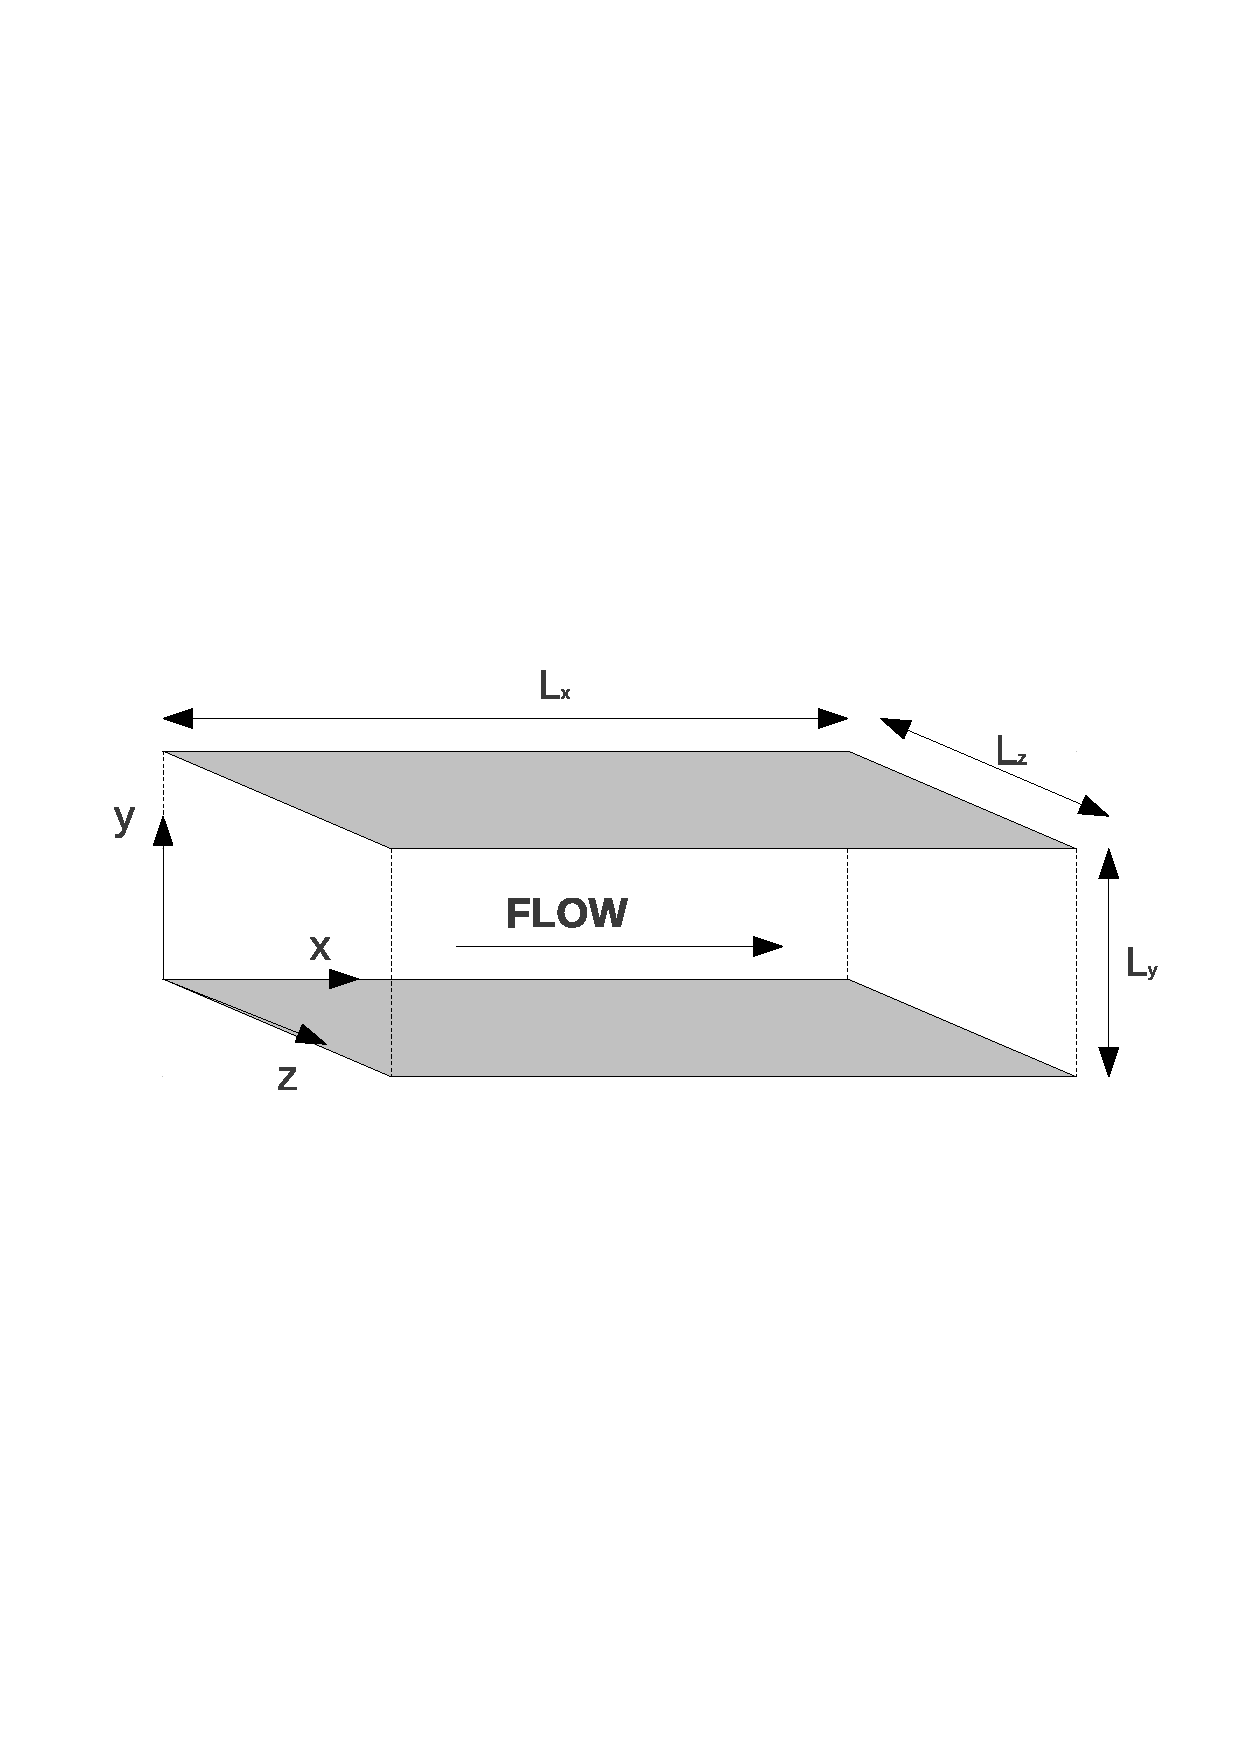
\includegraphics[width=0.8\linewidth]{dns_config}
\caption{Channel flow geometry.}
\label{pic:configuration}
\end{figure}

%A dimensionless velocity or Reynolds number of
%$Re_\text{bulk} = 3300$, based on the mean centreline velocity and
%$Re_{\tau}=183$, based on the wall shear velocity were chosen which
%offers a good comparison to a previous to statistics obtained by
%\citet{kmm87} as well as some guidance in referrence to mesh design
%due to other studies. The applied mesh uses about 768\,000 grid
%points ($ 80 \times 120 \times 80 $ in $x$,\,$y$,\,$z$). Nevertheless, all
%essential scales of turbulence are resolved on the computational grid
%and no subgrid model is used. Figure \ref{pic:mesh} shows one of the
%80 $z$-planes of the used mesh. \

%=============================================================================
\section{Parameters}

To match \citet{kmm87} we will aim for a bulk flow Reynolds number
based on the centreline mean speed $U$ and channel half-height
$\delta=L_y/2$ of $\Rey_\delta=U\delta/\nu=3300$.  For this flow the
associated Reynolds number based on the friction velocity
$u_\tau=(\tau_w/\rho)^{1/2}$ and half-height is
$\Rey_\tau=u_\tau\delta/\nu=183$. (It is worth noting that the
relationship between the bulk and friction Reynolds numbers for
turbulent flows is empirically based. For channel flow, a reasonable
approximation is given by $\Rey_\delta/\Rey_\tau=2.5\ln\Rey_\tau+5$,
while for turbulent flow in a pipe of diameter $D$, Blasius'
correlation $\Rey_\tau=u_\tau D/2\nu=99.44\times10^{-3}\Rey_D^{7/8}$
is quite good at moderate Reynolds numbers.)

\citet{kmm87} used domain extents of $L_x=4\pi\delta$ and
$L_z=2\pi\delta$ but for illustrative purposes we will choose the
smaller sizes $L_x=2\pi\delta$ and $L_z=\pi\delta$. We will find that
the turbulence statistics examined are apparently little affected by
this reduction in domain size, but the cost of simulation is
significantly reduced.  Since we will use Fourier expansions in the
$z$ direction we will have the basic spanwise wavenumber
$\beta=2\pi/L_z=2$.  This is set below by the simulation token
\texttt{BETA = 2}.

We will choose second-order time integration, usually the best
compromise between stability and accuracy.  (This is set below by the
token \texttt{N\_TIME = 2}, which could actually be omitted from the
session file since that is the default value.)

We need to choose a spectral element polynomial order. Values around 9
provide a good compromise between speed and accuracy for this
code. This is set with the token \texttt{N\_P = 10} (the number of
points along the edge of an element, one more than the polynomial
order).  Sometimes in what follows we will also approximate the
typical number of mesh divisions along the the edge of an element as
10, although the sharp-eyed reader will note that it should logically
be 9.

We need to choose the kinematic viscosity, $\nu$. We aim to have
$\Rey_\delta=3300$. It is good simulation/numerical practice to aim
for a characteristic velocity scale of unity, as well as a
characteristic mesh length scale of unity. In this case these goals
imply that we aim for a centreline mean speed $U\simeq1$ and our
channel half-height $\delta=1$.  With these choices we are left with
\[
  \nu = \Rey_\delta^{-1} = 303 \times 10^{-6},
\]
which is set by the simulation token \texttt{KINVIS = 303e-6}.

When using periodicity in the streamwise direction, a body force is
required in order to maintain the flow.  This is needed because the
pressure as well as the velocity is required to be
streamwise-periodic. The required body force per unit mass
(\ie acceleration) is calculated from a time-average force balance in
$x$-direction for the entire channel
\begin{eqnarray*}
 \rho \times f_x \times
  \underbrace{\cancel{L_x} \times L_y \times \cancel{L_z}}_{\text{channel
    volume}}  &=& 2 \times \tau_w \times \underbrace{\cancel{L_x} \times
    \cancel{L_z}}_{\text{one wall surface}} \\ 
   \rho \times f_x \times \delta & = & \tau_w\\
    \frac{f_x\delta}{U^2} & = & \left(\frac{u_\tau}{U}\right)^2 = 
    \left(\frac{\Rey_\tau}{\Rey_\delta}\right)^2
  \label{eq:force_balance}
\end{eqnarray*}
where $\tau_w$ is the time-average wall shear stress.  With $\rho =
\delta = U= 1$ and (from correlation/previous results)
$\Rey_\tau=183$, $\Rey_\delta=3300$, the required value is
\[
  f_x = 3.08 \times 10^{-3} .
\]
This will be set with the token \texttt{CONST\_X = 3.08e-3} in the 
\texttt{<FORCE>} section.  Note that if
required for body forces in the $y$ or $z$ directions there are
corresponding tokens \texttt{CONST\_Y} and \texttt{CONST\_Z} respectively 
(see section~\ref{sec.dns_ff} for other types of forcing).
These body forces are added to the component momentum equations (the
\NavSto\ equations).  Also note that the code is written assuming
$\rho=1$.

The friction velocity $u_\tau=(\tau_w/\rho)^{1/2}\equiv
U\Rey_\tau/\Rey_\delta=55.5\times10^{-3}$, and the viscous wall length
scale $l_w=\nu/u_\tau=5.46\times10^{-3}$.

%============================================================================
\section{Mesh design}
\label{sec.meshdesign}

In designing the mesh for the channel flow, rules of thumb established
in related studies \citep{pio97,kmm87,blsc03} have been
considered. All mentioned coordinates are with respect to coordinate
system established in this work. Thus, $x$ is the streamwise
direction, $y$ the wall-normal and $z$ the spanwise direction ---
Fourier expansions are always used in the $z$ direction.


\citet{kmm87} used $\Delta x^+ =\Delta x / l_w = 12$, $y^+ = 0.05$ (at
the wall) and $\Delta z^+ = 7$ in their study. \citep{pio97} proposed
similar values with $\Delta x^+ = 15$, $\Delta y^+ < 1|_\text{wall}$
and $\Delta z^+ = 6$.
%Referencing \citeauthor{pio97}, \citet{blsc03} used a mesh with
%$\Delta x^+ = 85$, $y^+ = 10$, $\Delta z^+ = 32$ for the individual
%element with $8 \times 8$ GLL nodes in $(x,y)$.

The wall-normal part of the spectral element mesh design strategy for
wall-resolved LES described by \citet{blsc03} is to terminate the
element closest to the wall at $y^+=10$, the second element at
$y^+\simeq35$, then use a geometric progression of sizes to reach the
flow centreline (one has to choose the number of elements and
geometric expansion factor).  This ensures there is good resolution in
the viscous-dominated wall layer as well as the buffer layer
($10<y^+<35$), where turbulent energy production is greatest.
Nevertheless, here, the second element layer is reduced to $y^+ = 25$
in order to improve resolution in the middle of the buffer layer.

The first two element heights in the wall-normal direction are then
$\Delta y_1(10)=0.056$ and $\Delta y_2(25)=0.139$. For the remainder,
we use a geometric progression of four elements starting with an
initial height of $\Delta y = 0.139-0.056=0.083$ to reach the channel
centreline.  The total number of elements in the $y$-direction is 12.

Next considering the $x$-direction, the indicative mesh spacing is
$\Delta x^+=15$, corresponding to a length $\Delta x =
15\times5.46\times10^{-3}=81.9\times10^{-3}$.  The number of grid
points needed to cover the domain extent in the $x$-direction is then
of order $N_x=2\pi/\Delta x=76.7$.  For a mesh with \verb|N_P=10| we
need of order 8 elements.  So our $(x,y)$ spectral element mesh is now
of size $8\times12=96$ elements.

Finally considering the $z$ direction, we have $L_z=\pi$ and want
$\Delta z^+\simeq7$, or $\Delta
z\simeq7\times5.46\times10^{-3}=38.2\times10^{-3}$.  The implied
number of $z$ planes is then of order $\pi/38.2\times10^{-3}=82.2$.
We need an integer number of planes which must be even (one prime
factor of 2) and other allowable prime factors of 3 and 5.  80 planes
seems convenient so we choose \verb|N_Z = 10|.  Note that means we
could run on either a single processor in serial execution or 2, 4, 8,
10, 20 or 40 in parallel.  There will be 40 Fourier modes.

%Figure \ref{pic:profile}(a) illustrates these rules in question and
%allows to compare them to the mesh ultimately used (b) showing the
%average streamwise velocity.
%\begin{figure}[b]
%\centering
%\subfigure[ ]
%{\includegraphics[height=50mm]{dns_profile.ps}}
%\subfigure[ ]
%{\includegraphics[height=50mm]{dns_wall_profile.ps}}
%\caption{Mesh design in the near wall region (a) and real distribution (b)}
%\label{pic:profile}
%\end{figure}

The mesh can be created using the provided tool \texttt{rectmesh}
which reads from an input file containing two blocks with all grid
lines in $x$ and $y$ separated by an empty line. The output from
running \verb|rectmesh| will be a valid \Semtex\ session file but which
will generally need some editing. 

{\small
\begin{verbatim}
rectmesh [options] mesh.inp > sessionfile
\end{verbatim}
}

A \verb|rectmesh| input file for this case is as follows: {\small
\begin{verbatim}
-3.14159265358979
-2.35619449019234
-1.5707963267949
-0.785398163397448
0.0000
0.785398163397448
1.5707963267949
2.35619449019234
3.14159265358979

-1.0
-0.944
-0.861
-0.745
-0.575
-0.330
0.0
0.330
0.575
0.745
0.861
0.944
1.0
\end{verbatim}
}

Once this file is built, all the above mentioned parameters can be
changed to their desired value. Also, the boundary conditions have to
be named and set into place.  We use wall boundary conditions on the
upper and lower edges of the domain, and edit the \verb|<SURFACES>|
section to obtain periodicity in the streamwise direction. Here is the
example input file for this particular case (which is much the same as
the \verb|chan3| session file in the \verb |mesh| directory):

{\small
\begin{verbatim}
################################################################
#  96 element channel flow, for Re_bulk = 3300, Re_tau = 183

<FIELDS>
	u v w p
</FIELDS>

<USER>
    u = 1.0-y*y
    v = 0.0
    w = 0.0
    p = 0.0
</USER>

<TOKENS>
    N_TIME  = 2
    N_P     = 10
    N_Z     = 80
    BETA    = 2.0
    D_T     = 0.01
    T_FINAL = 800
    N_STEP  = int(T_FINAL/D_T)
    KINVIS  = 303e-6
    IO_CFL  = 100
    IO_HIS  = 100
    AVERAGE = 2
</TOKENS>

<FORCE>
    CONST_X = 3.08e-3
</FORCE>

<GROUPS NUMBER=1>
    1	w	wall
</GROUPS>

<BCS NUMBER=1>
    1	w	4
        <D> u = 0.0 </D>
        <D> v = 0.0 </D>
        <D> w = 0.0 </D>
        <H> p       </H>
</BCS>

<NODES NUMBER=117>
    1	       -3.14159             -1              0
  ...
  117	        3.14159              1              0
</NODES>

<ELEMENTS NUMBER=96>
    1	<Q>    1    2   11   10    </Q>
  ...
   96	<Q>  107  108  117  116    </Q>
</ELEMENTS>

<SURFACES NUMBER=28>
    1    1    1    <B> w </B>
    2    2    1    <B> w </B>
    3    3    1    <B> w </B>
    4    4    1    <B> w </B>
    5    5    1    <B> w </B>
    6    6    1    <B> w </B>
    7    7    1    <B> w </B>
    8    8    1    <B> w </B>
    9   89    3    <B> w </B>
   10   90    3    <B> w </B>
   11   91    3    <B> w </B>
   12   92    3    <B> w </B>
   13   93    3    <B> w </B>
   14   94    3    <B> w </B>
   15   95    3    <B> w </B>
   16   96    3    <B> w </B>
   17    8    2    <P>   1      4       </P>
   18   16    2    <P>   9      4       </P>
   19   24    2    <P>  17      4       </P>
   20   32    2    <P>  25      4       </P>
   21   40    2    <P>  33      4       </P>
   22   48    2    <P>  41      4       </P>
   23   56    2    <P>  49      4       </P>
   24   64    2    <P>  57      4       </P>
   25   72    2    <P>  65      4       </P>
   26   80    2    <P>  73      4       </P>
   27   88    2    <P>  81      4       </P>
   28   96    2    <P>  89      4       </P>
</SURFACES>

<HISTORY NUMBER=1>
	1	0.0	0.0	0.0
</HISTORY>
\end{verbatim}
}


%=============================================================================
\section{Initiating and monitoring transition}
\label{sec.transition}

The critical bulk Reynolds number for linear instability of channel
flow is $\Rey_c = 5772$ but turbulence can typically be maintained down
to lower values (and here we are aiming at $\Rey_\delta=3300$) if
transition is obtained. Our strategy here will be to start from a
laminar flow profile and add some white noise to obtain transition.
This is done using the following single line to generate an initial
condition: {\small
\begin{verbatim}
compare chan | noiz -p 0.1 > chan.rst
\end{verbatim}
}

Here, the command-line value 0.1 represents the standard deviation of
the normal/Gaussian distribution from which the noise is derived using
a pseudorandom number generator and is therefore quite large compared
to an average velocity of $U=1$. It is necessary, since our Reynolds
number is here below the critical value, to assure a sufficient amount
of disturbance to initiate transition to a turbulent state. If the
Reynolds number were above the critical value, any perturbation level
above machine noise level should eventually produce transition --- it
just depends on how long you are prepared to wait. We note that
channel flow is a case for which it is relatively easy to obtain
transition to turbulence without carefully manipulating the noise
level, or restricting the time step.

In order to monitor transition, a very useful diagnostic is to monitor
the evolution of kinetic energies in all Fourier modes.  Transition
should be easy to see as a moderately rapid increase in turbulent
energy within small scales that are represented by higher wave
numbers. Figure~\ref{pic:modal_en}(a) shows the transition for the
mentioned channel flow. Figure~\ref{pic:modal_en}(b) indicates that
the resolution is adequate due to a separation of about three and a
half decades between the highest and smallest wave number. An increase
of energy within the highest wave numbers would also indicate an
under-representation because of aliasing of the energy of higher modes
back into the resolved frequency domain (which is the underlying
reason for the plateau seen at the highest wavenumbers in
figure~\ref{pic:modal_en}(b)).

\begin{figure}
  \begin{center}
    \begin{tabular}{cccc}
    \raisebox{32ex}{(a)}&
    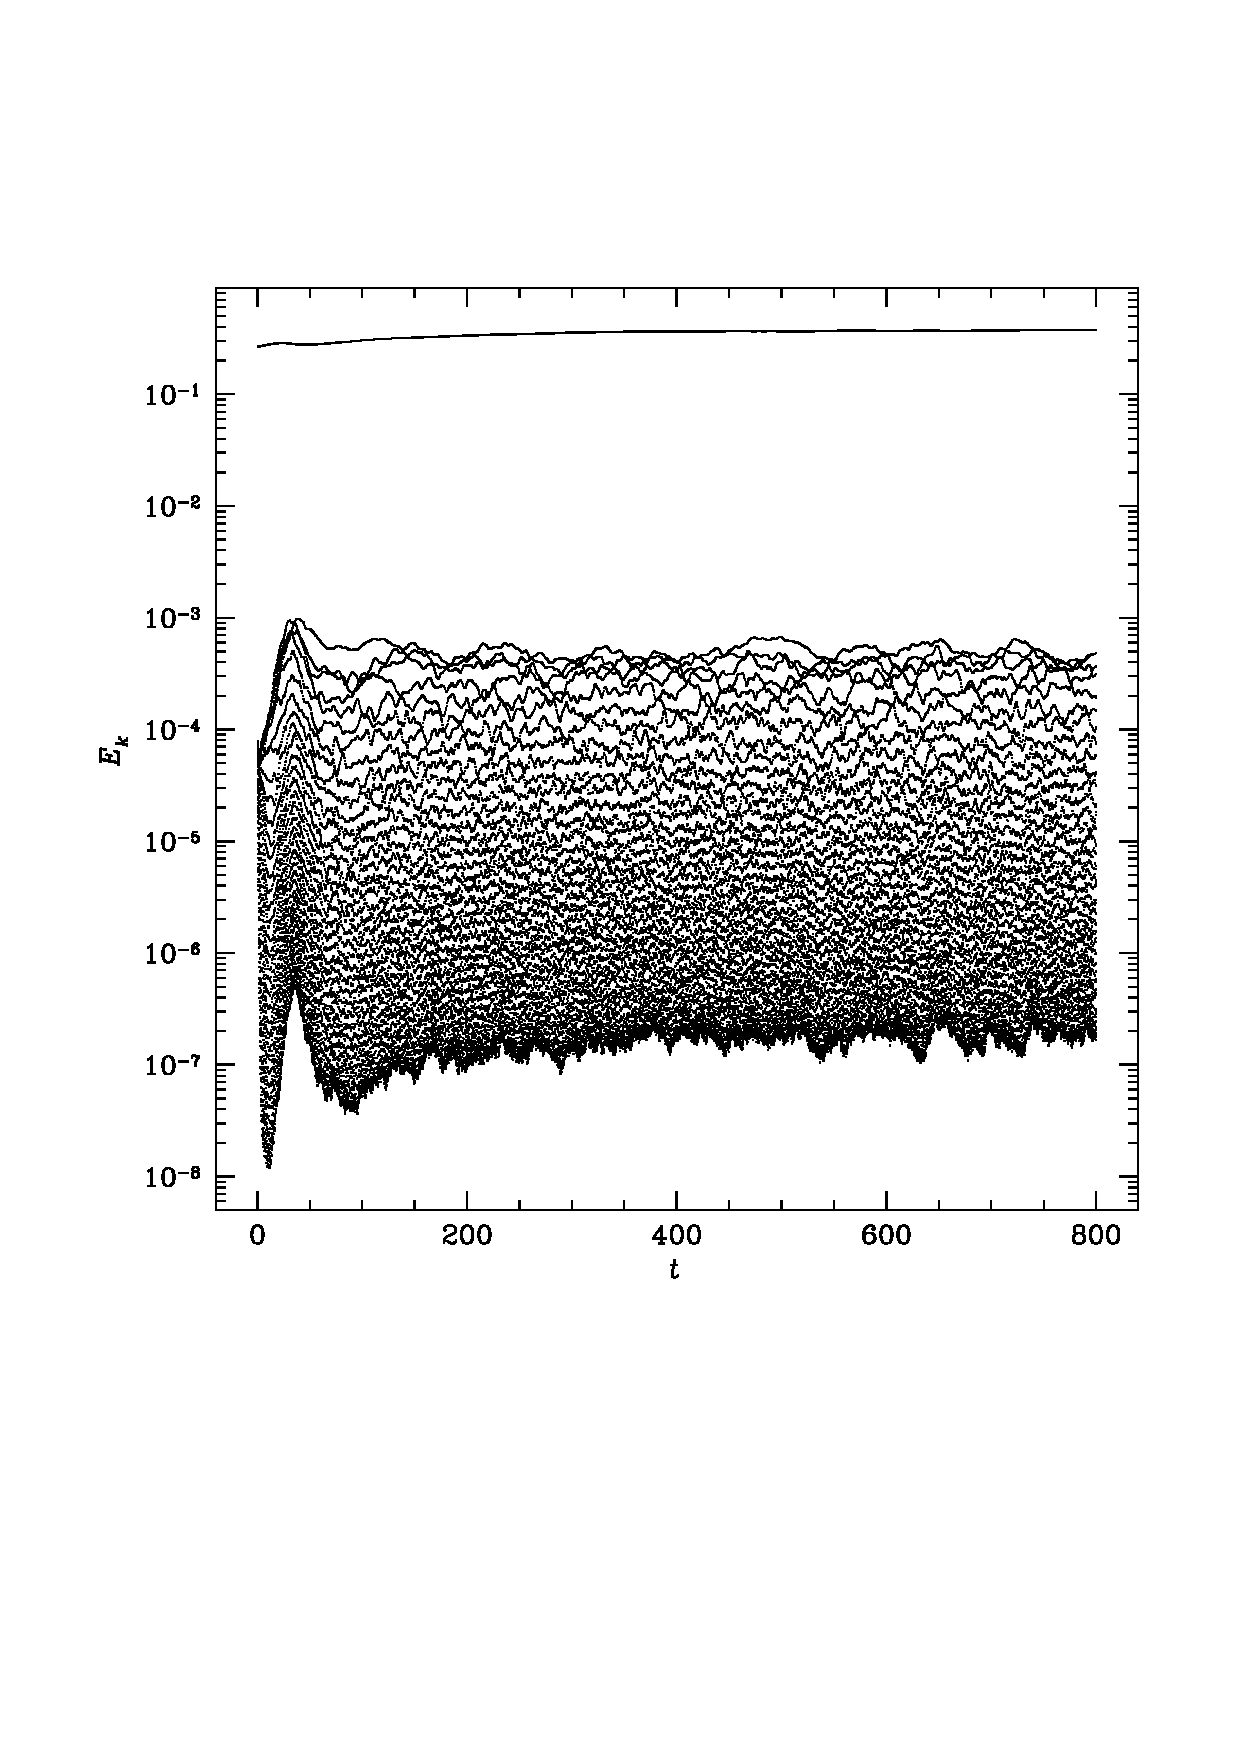
\includegraphics[height=0.2462\textheight]{chan3mdl}&
%   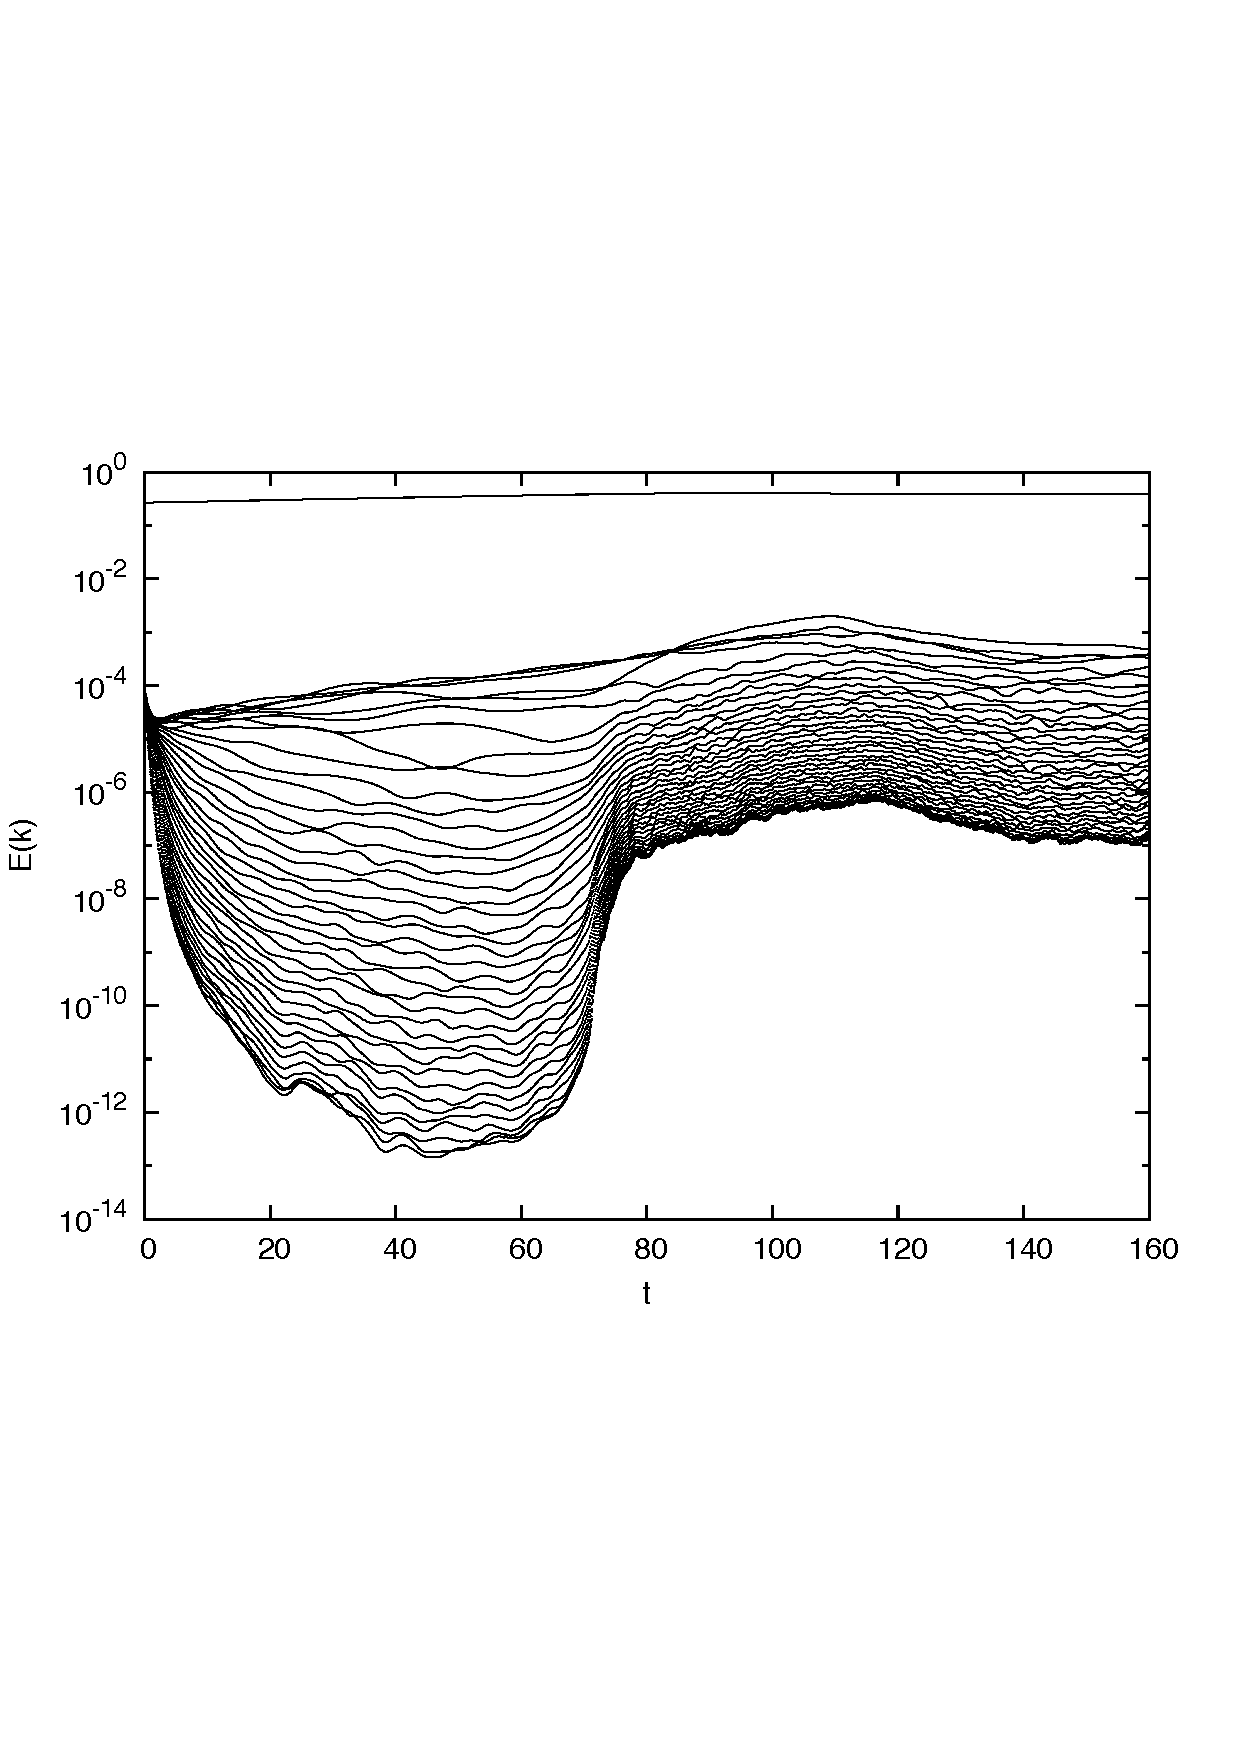
\includegraphics[height=0.22\textheight]{dns_modal_t}&    
    \raisebox{32ex}{(b)}&
    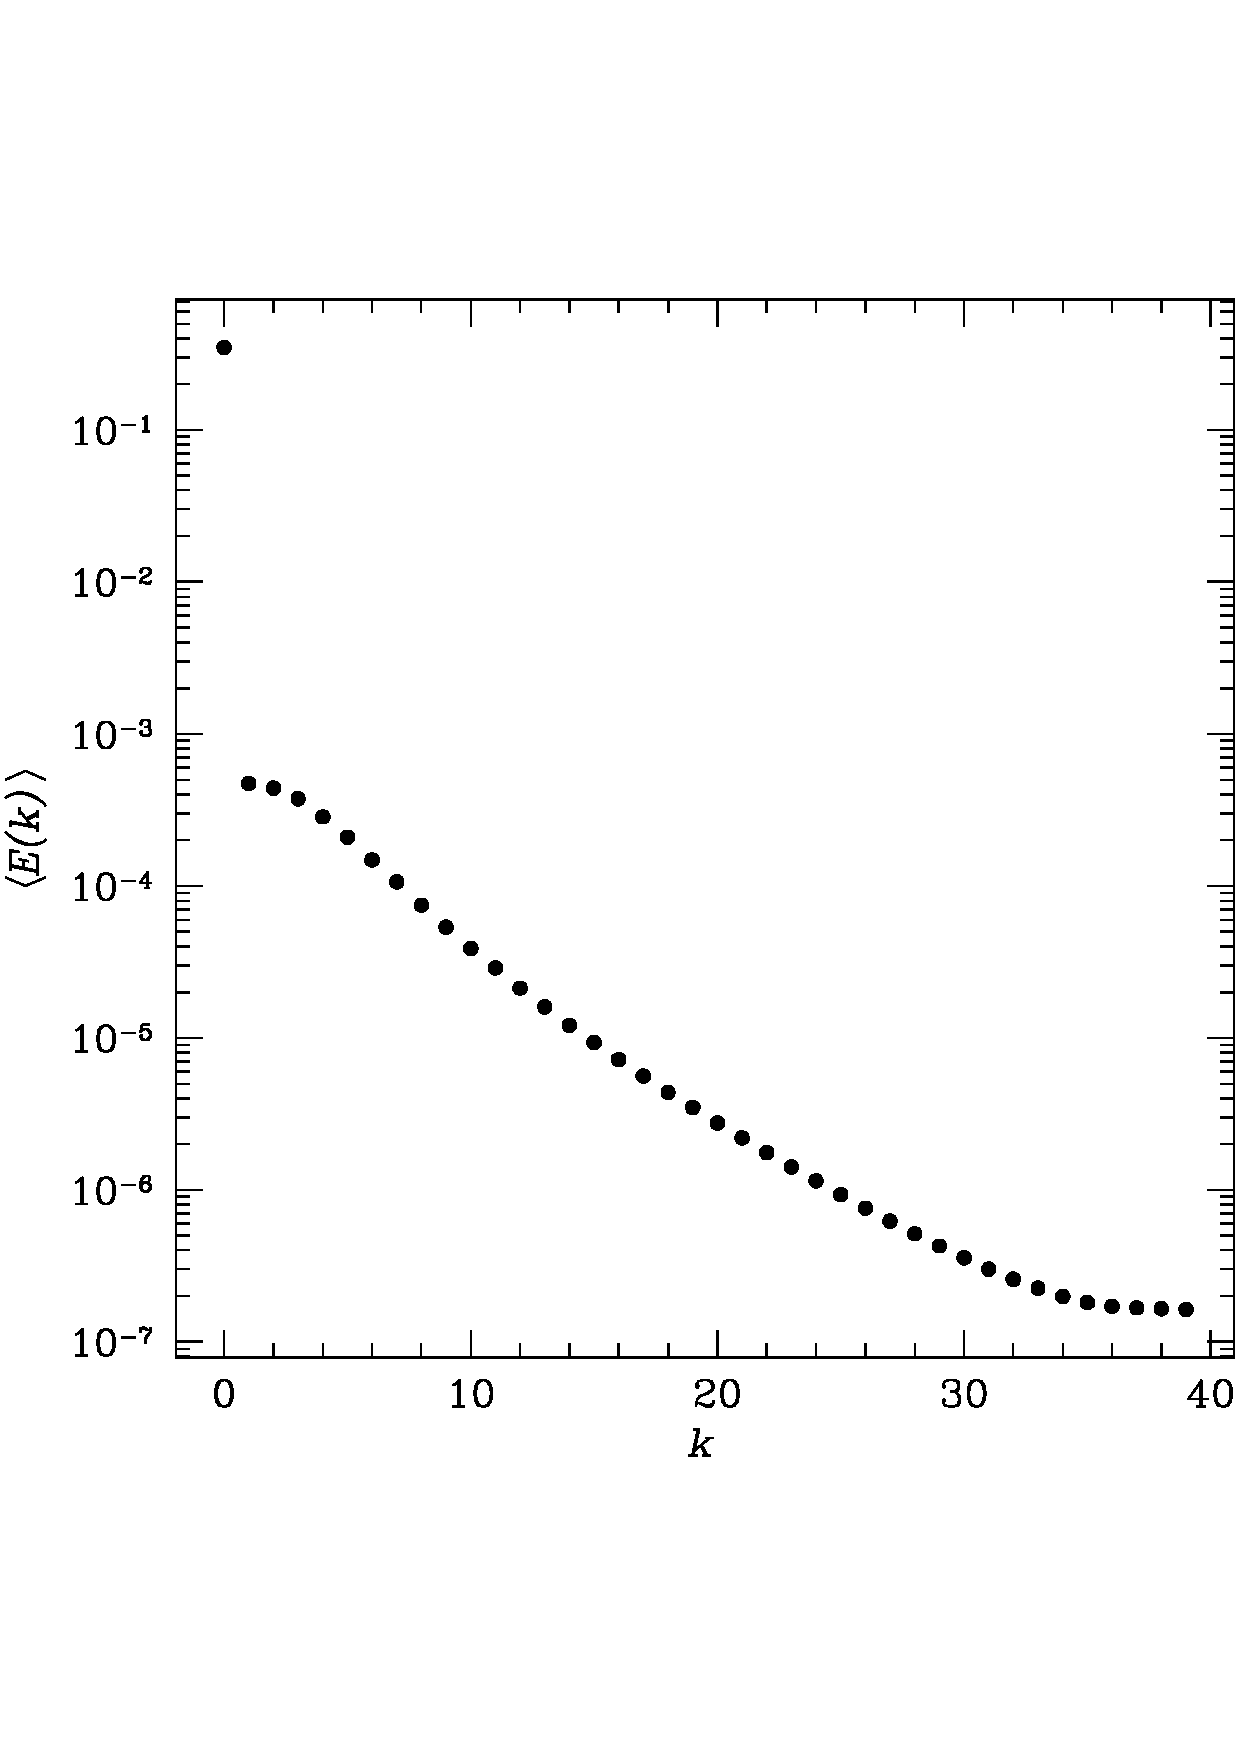
\includegraphics[height=0.25\textheight]{chan3modav}
%   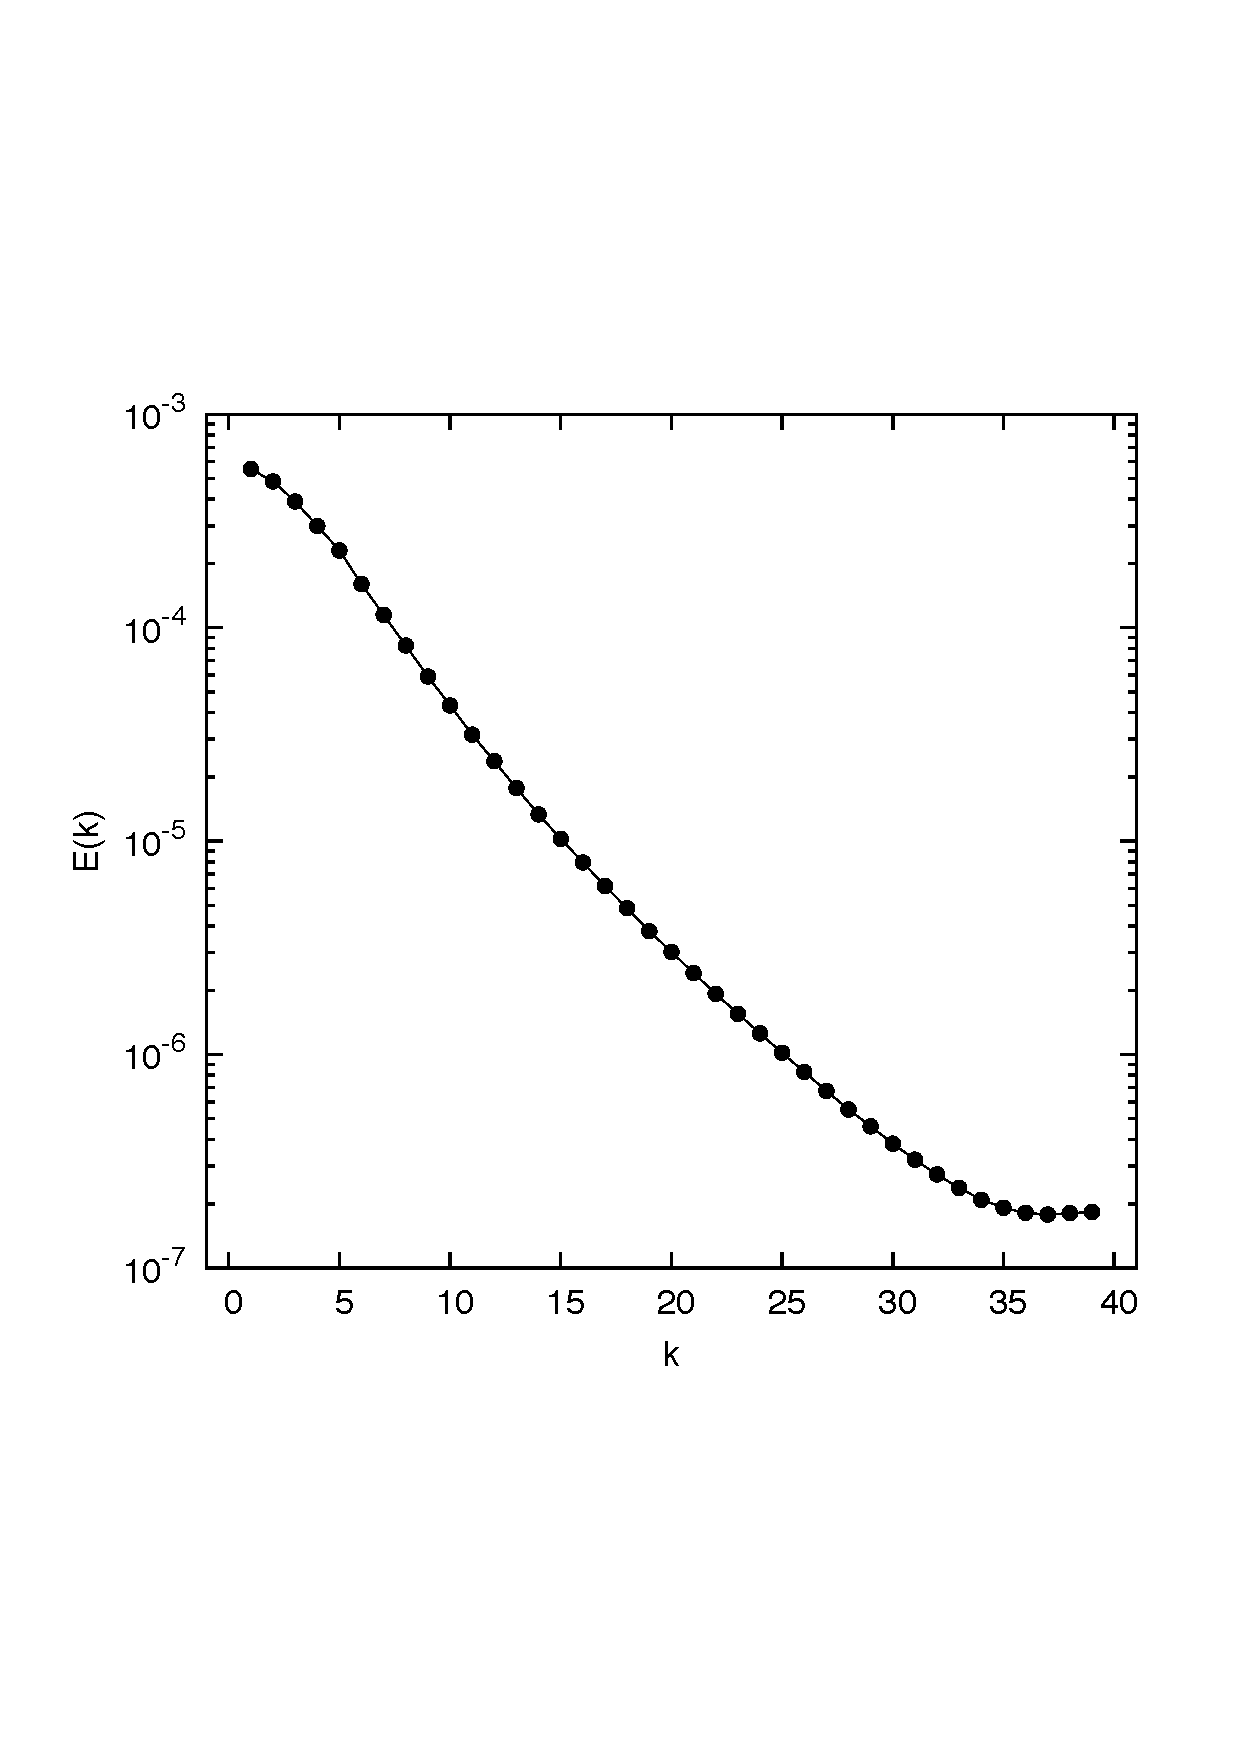
\includegraphics[height=0.22\textheight]{dns_modal_k}    
    \end{tabular}
  \end{center}
 \caption{Modal energies for (a) the individual wave numbers over time
   and (b) by wavenumber.  These images were prepared using
   \SM\ macros.}
 \label{pic:modal_en}
\end{figure}

Figure~\ref{pic:modal_en}(a) shows the evolution of kinetic energies
in the 40 Fourier modes represented.  By way of interpretation, the
mode with highest energy (here, and typically) is mode~0, which
represents the \twod\ or $z$-average flow.  All the other modes start
off with much the same energy, which is a result of having chosen to
pollute all modes equally when using the \verb|noiz| utility (often,
one would just pollute mode~1 and allow convolution to distribute
energy to all other modes --- this gives a more gentle perturbation).
The highest modes typically decay rather rapidly initially, with the
lower modes either slowly losing or (as here, gaining) energy.  Also
the energy in mode~0 here increases a little over time, partly because
the initial condition here actually had a lower volumetric flow rate
than the equilibrium turbulent flow. At $t\approx70$ the flow makes a
transition to a turbulent state, typically signalled by the higher
modes gaining energy fairly rapidly until a quasi-equilibrium is
reached. Eventually the flow settles to a statistical equilibrium at
$t\approx600$.  Figure~\ref{pic:modal_en}(b) shows the temporal
average values of energies in the various Fourier modes.  (The
\SM\ macros \verb|moden| and \verb|modav| were used to plot
figure~\ref{pic:modal_en}.)

At the end of this simulation, the flow should be in an approximately
statistical stationary state.  Check the $x$-component tractive force
given at the end of \verb|chan.flx| (which should be around 0.0388).
This is the tractive force per unit domain width in the $z$-direction
(see \S\,\ref{sec.flux}).  That ought to closely balance the total
body force per unit width, which is
$f_x\times2\times2\pi=303\times10^{-6}\times2\times2\pi=0.0387$.  Since
the flow is turbulent and driven by a constant body force, both the
bulk velocity (volumetric flow rate per unit area) and wall tractions
will fluctuate somewhat in time, and we should really compare the
time-average tractive force with the body force, but evidently the
single-time outcome is quite close.  The agreement should also depend
on the spatial and temporal resolution of the simulation, but the
resolution suggested in the session file is quite good for the
Reynolds number employed.

%=============================================================================
\section{Timestepping order, restarting, and parallel execution}
\label{sec.restart}

\Semtex's \verb|dns| can run with first, second, or third-order
accurate timestepping according the token \verb|N_TIME|, whose default
value of 2 implies second-order timestepping, which is generally the
best choice.  However, CFL stability declines somewhat as timestepping
order increases, and if in any case you know that you are headed
towards a steady-state outcome, \verb|N_TIME=1| might be a better
choice so that comparatively larger timesteps could be used while
still maintaining CFL stability.  These choices also have a subtle
interaction with restarting (which can be accomplished by copying or
moving \verb|session.fld| to \verb|session.rst| and running again),
since only a single field dump is read from \verb|session.rst|,
meaning that the first subsequent timestep can only be first-order
accurate (the second can be second-order accurate, etc., up to the
order you are running with).  For a turbulent flow this effect has
only minor overall significance, but it can lead to small disruptions
at every restart for a steady or periodic flow; generally it is an
effect to be aware of rather than concerned about.

As will be pointed out immediately below, when restarting with token
$\texttt{AVERAGE}>0$, \verb|dns| will also attempt to read in
\verb|session.avg| in order to continue accumulating statistics.

%=============================================================================
\section{Flow statistics}
\label{sec.stats}

Flow statistics can be collected by setting the \verb|AVERAGE| token
to non-zero values 1, 2 or 3 (here a value of 2 was used, see below).
See also \S\,\ref{sec.average}.  To obtain statistical convergence it
is necessary to average over a sufficiently long time, just as would
be the case in a physical experiment. Statistics are updated every
\verb|IO_HIS| simulation steps (here, every 100 steps).  In the
present case, the total averaging time was chosen to be 400, which
represents of order 60 `wash-through' times, since the domain length
is $2\pi$ and the bulk flow speed $U=1$.  Since the time between data
updates is $100\times0.002=0.2$ there are a total of $400/0.2=2000$
averaging buffer updates.

Once the simulation is run, a \texttt{.avg} file is produced. For
\verb|AVERAGE=1|, statistics for the represented fields are collected,
\ie $\langle u\rangle$, $\langle v\rangle$, \ldots, $\langle
p\rangle$.  For \verb|AVERAGE=2|, averages of velocity field products
are stored too, \ie $\langle uu\rangle$, $\langle uv\rangle$, etc.
For \verb|AVERAGE=3|, additional products are collected to allow
computation of terms in the fluctuating energy equation.  Note that it
is necessary to calculate Reynolds stresses and energy equation terms
in post-processing (\eg $\langle u'v'\rangle = \langle
uv\rangle-\langle u\rangle\langle v\rangle$).  Note also that if
\verb|.avg| files exist, they are read in at start of execution of
\verb|dns| to initiate averaging buffers: the \verb|Step| value in the
file's header stores the number of averages obtained to date.

Having collected statistics, our next step is to calculate the
Reynolds stresses and to average in $x$- and $z$-direction. To
illustrate the possible processing, here is an example shell script:

{\small
\begin{verbatim}
#!/bin/bash

# temporary files
FTNZ='/tmp/chan_nz1'
FTRS='/tmp/reynolds-stress.xy'
FRSY='./reynolds-stress.y'

# average field results in z
project -z1 chan.avg > /tmp/chan.avg.xy

# calculate reynolds-stresses (xy-plane)
rstress /tmp/chan.avg.xy > $FTRS

# new input file with NZ=1
LNZ=$(cat chan | grep N_Z -n | awk -F: '{print $1}')
sed '$LNZs/.*/  N_Z    = 1/' <chan >$FTNZ

# average reynolds-stresses in x
rayavg npts navg y_0 x_0   y_0 x_1 dy dx $FTNZ $FTRS >  $FRSY
rayavg npts navg y_0 x_1   y_0 x_2 dy dx $FTNZ $FTRS >> $FRSY
...
rayavg npts navg y_0 x_n-1 y_0 x_n dy dx $FTNZ $FTRS >> $FRSY

# PLOTTING -- make a gnuplot script if you like:
gnuplot ~/scripts/plot_rstress.gpl;
\end{verbatim}
}

Figure \ref{pic:u_wall} shows the mean velocity profile for the
channel flow in comparison to data from \citet{kmm87}. The dashed
lines are representing the linear respectively logarithmic part of the
law of the wall.  Figure \ref{pic:rms_global} show rms Reynolds stress
values in friction velocity units with comparison to data from
\citet{kmm87}.  Quite good agreement is evident.

\begin{figure}
\centering
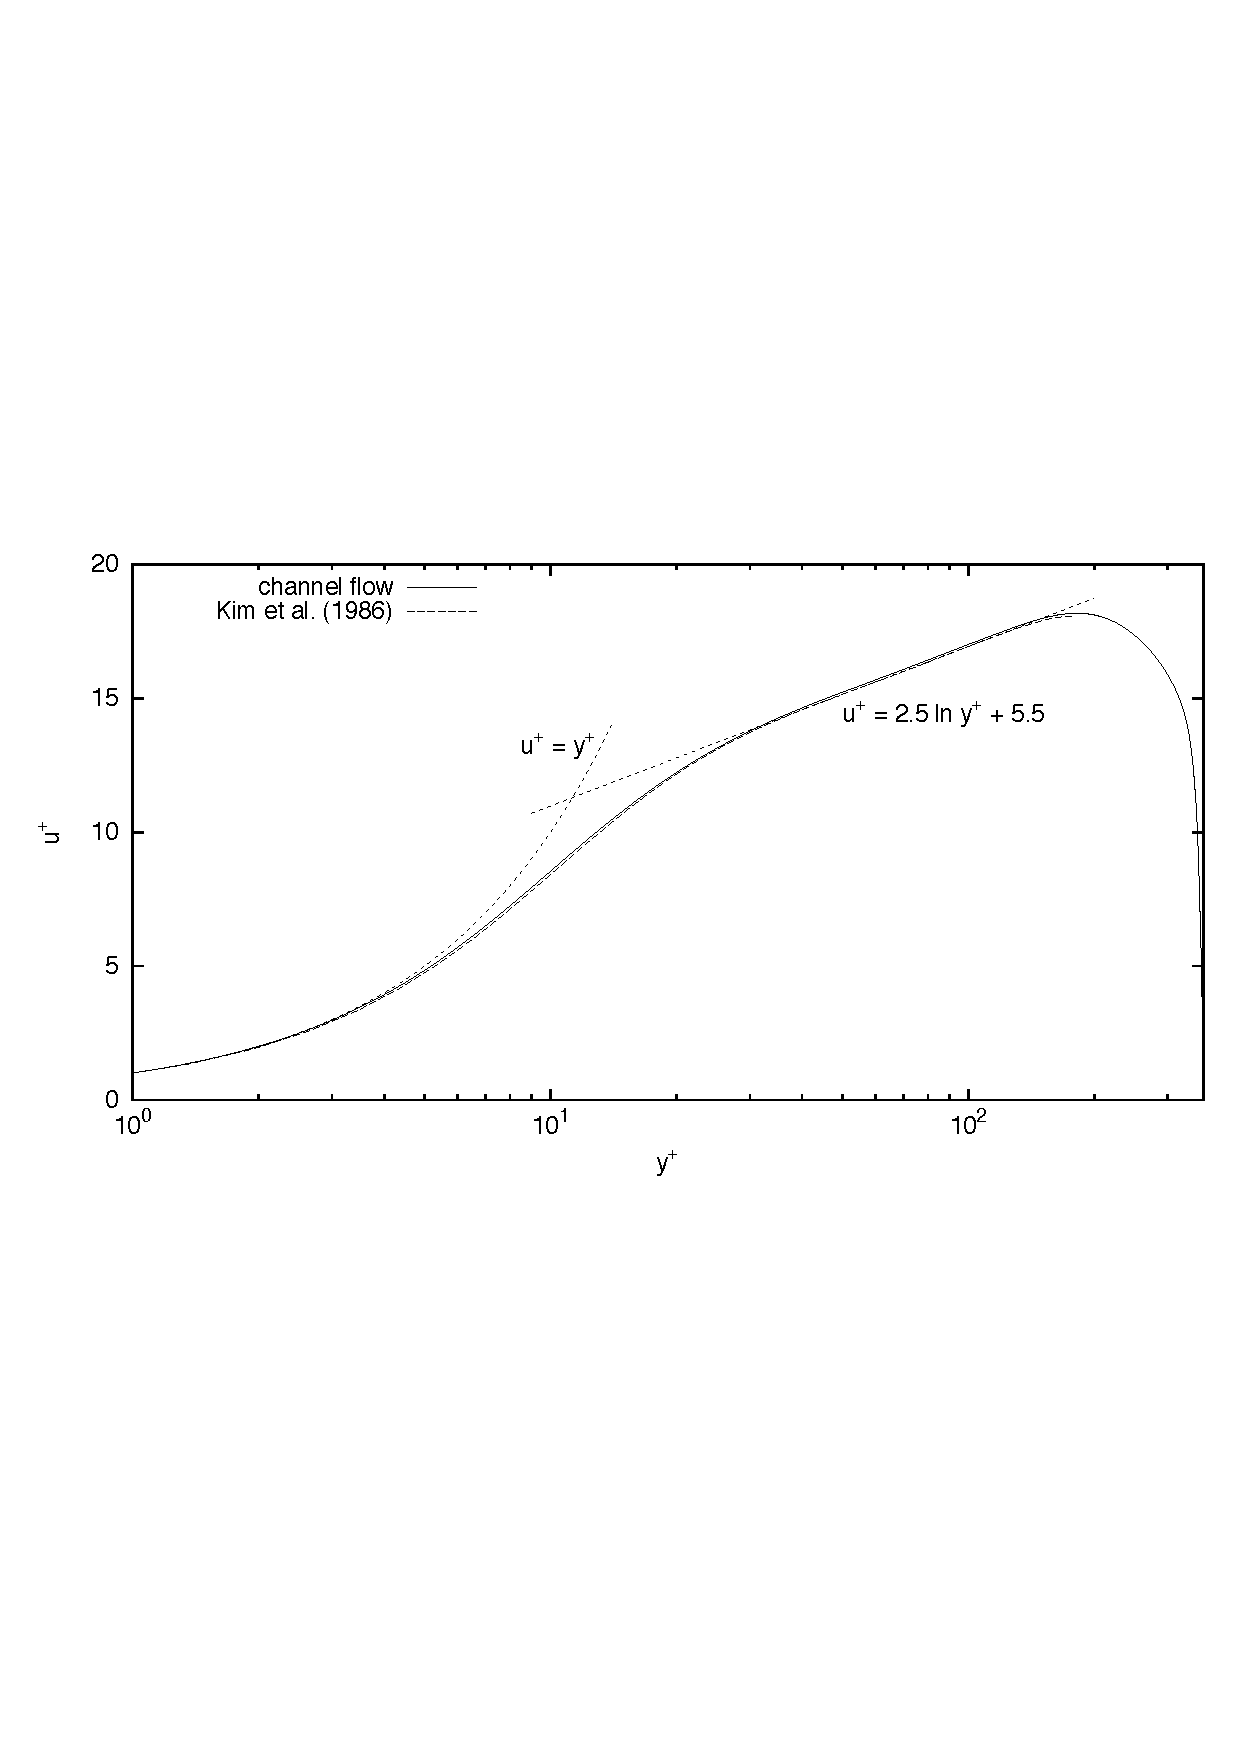
\includegraphics[height=0.28\linewidth]{dns_u_wall}
\caption{Mean velocity profile of the channel flow compared to the law
  of the wall and data from \citet{kmm87}}
\label{pic:u_wall}
\end{figure}

\begin{figure}
\begin{center}
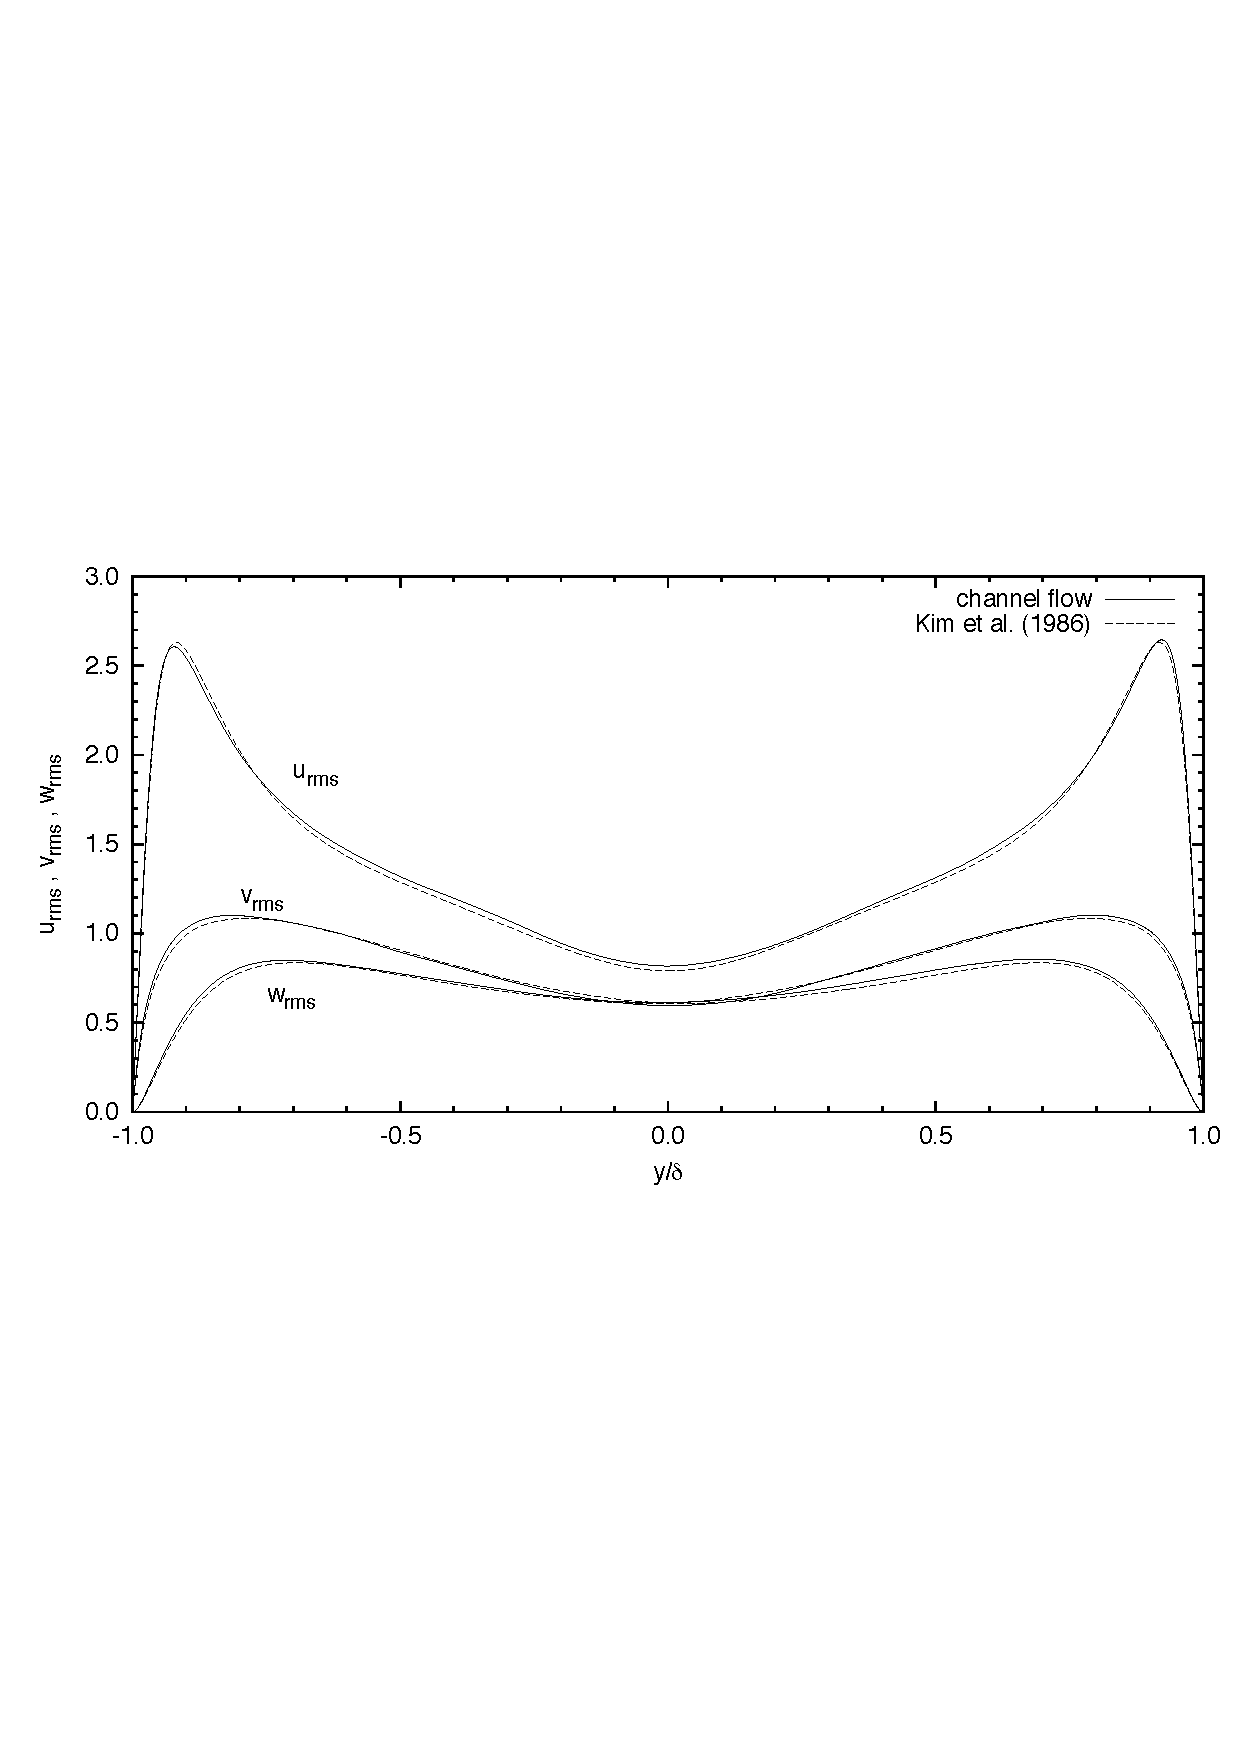
\includegraphics[height=0.27\linewidth]{dns_rms_global}\\
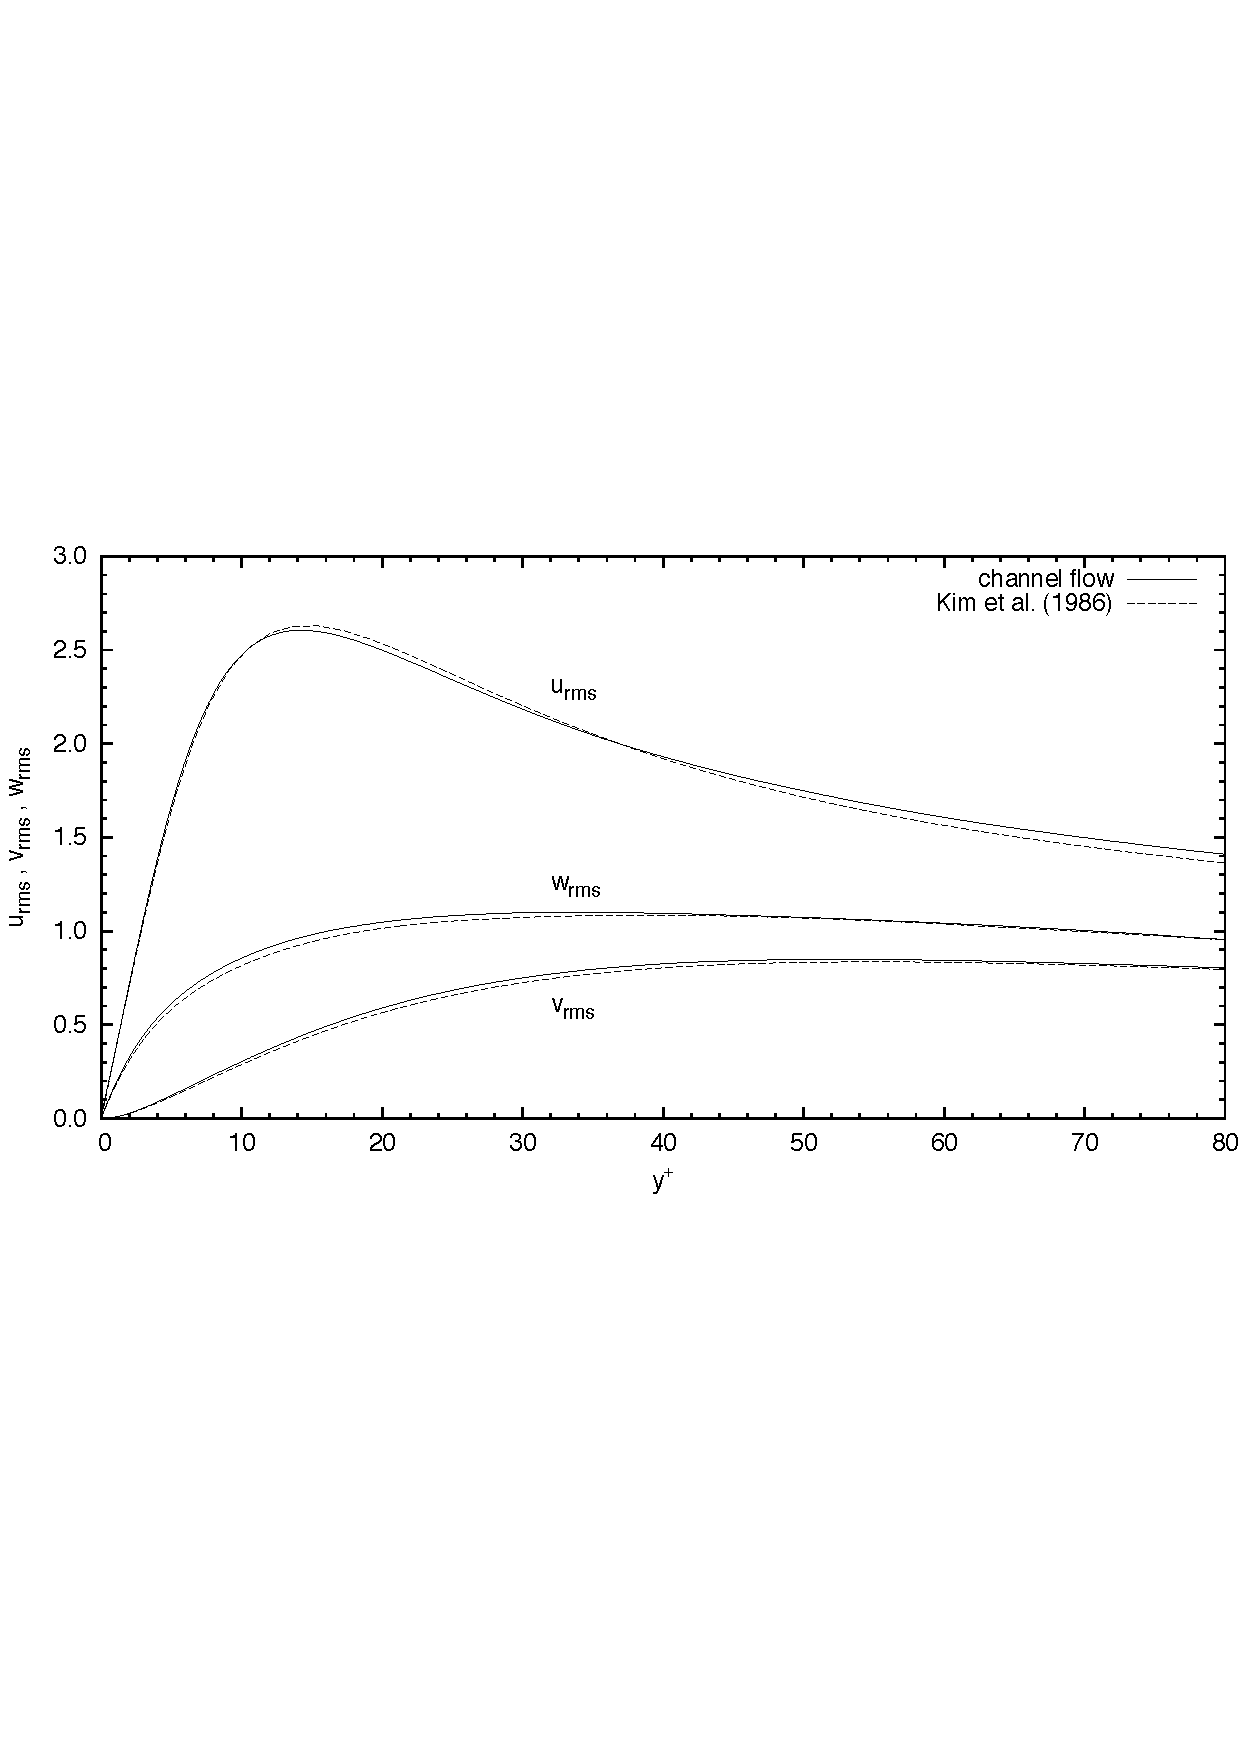
\includegraphics[height=0.27\linewidth]{dns_rms_wall}
\end{center}
\caption{ Root-mean-squares velocity fluctuations in global
  coordinates normalised by the wall shear velocity
  $u_{\tau}$. Comparison to data from \citet{kmm87}.}
\label{pic:rms_global}
\end{figure}

\emph{Finally (though it is very important), we should note that one
could run this simulation either on a single processor, or, using MPI,
on up to 40 processors (and perhaps have sped up execution by up to a
factor of 40!).  Please see the discussion of \S\,\ref{sec.mpi} for
further information.}

%%%%%%%%%%%%%%%%%%%%%%%%%%%%%%%%%%%%%%%%%%%%%%%%%%%%%%%%%%%%%%%%%%%%%%%%%%%%%

\clearpage
\addcontentsline{toc}{chapter}{References}
\bibliographystyle{dcu}
\bibliography{userguide}

%%%%%%%%%%%%%%%%%%%%%%%%%%%%%%%%%%%%%%%%%%%%%%%%%%%%%%%%%%%%%%%%%%%%%%%%%%%%%
\end{document}
